\documentclass[print]{dissertation}

\usepackage{amsmath}
\usepackage{amssymb}
\usepackage{mathabx}
\usepackage{bbold}
\usepackage{calc}
\usepackage{wasysym}
\usepackage{mathtools}
\usepackage{physics}
\usepackage{romannum}
%\usepackage{graphicx}
%\usepackage{hyperref}
%\usepackage{etoolbox}
%\usepackage{ifthen}
%\usepackage{cases}
%\usepackage{xstring}
%\usepackage{fullpage}
%\usepackage{environ}
%\usepackage{doi}
\usepackage{cleveref}

% Include PDFs %
%%%%%%%%%%%%%%%%
\usepackage{pdfpages}

%\hypersetup{
%	colorlinks,
%	linkcolor={BlueViolet},
%	citecolor={BlueViolet},
%	urlcolor={BlueViolet}
%}

% Tikz %
%%%%%%%%
\usepackage{tikz, tikz-cd}\usetikzlibrary{cd, calc, decorations.markings, shapes.geometric}
\usepackage{tikz}
\usetikzlibrary{shapes.geometric,arrows,matrix,calc,scopes,decorations.markings,intersections,arrows.meta,decorations.pathreplacing,angles,quotes,patterns,decorations.pathmorphing}

\newcommand{\inputtikz}[1]{%
%	\tikzsetnextfilename{#1}%
	\input{figs/#1.tex}%
}


% Math %
%%%%%%%%

\allowdisplaybreaks

\renewcommand{\vec}[1]{{\bf #1}}

\newcommand{\rU}{{\rm U}}
\newcommand{\rd}{{\rm d}}
\newcommand{\im}{\text{im}\,}
\newcommand{\la}{\langle}
\newcommand{\ra}{\rangle}
\newcommand{\sss}{\scriptstyle}
\newcommand{\ssss}{\scriptscriptstyle}
\newcommand{\bul}{\raisebox{1pt}{${\sss \bullet}$}}
\newcommand{\bulScr}{\raisebox{.5pt}{$\ssss \bullet$}}
\newcommand{\snum}[1]{\text{\small $#1$}}
\newcommand{\mc}[1]{\mathcal{#1}}
\newcommand{\mbb}{\mathbb}
\newcommand{\fr}[1]{\mathfrak{#1}}
\newcommand{\msf}[1]{\mathsf{#1}}
\newcommand{\tmsf}[1]{\tilde{\mathsf{#1}}}

\newcommand{\ub}{\underline}
\newcommand{\ZtZt}{\mbb Z_2\times\mbb Z_2}
\newcommand{\End}{{\rm End}}
\newcommand{\upup}[1]{\raisebox{0.5pt}[0pt]{$\sss{#1}$}}
\newcommand{\dodo}[1]{\raisebox{-1.2pt}[0pt]{$\sss{#1}$}}
\newcommand{\CC}[6]{\Big[{}^{\upup{#1}}_{\dodo{#4}}\, {}^{\upup{#2}}_{\dodo{#5}} \big| {}^{\upup{#3}}_{\dodo{#6}}\Big]}

% Cat theory
\newcommand{\ob}{{\rm ob}}
\newcommand{\rF}{{}^{\cat\!} F}
\newcommand{\lF}{{}^{\act\!\!} F}
\newcommand{\bF}{{}^{\bowtie\!} F}
\newcommand{\Dim}{{\rm FPdim}}
\newcommand{\cat}{\lhd}
\newcommand{\catb}{\lhd'}
\newcommand{\act}{\rhd}
\DeclareMathOperator{\actb}{\mathrlap{\hspace{1.2pt}\cdot}\rhd}
\newcommand{\Vect}{\mathsf{Vec}}
\newcommand{\Rep}{\mathsf{Rep}}
\newcommand{\Fun}{\mathsf{Fun}}
\newcommand{\Mod}{\mathsf{Mod}}
\newcommand{\TVect}{2\mathsf{Vec}}
\newcommand{\TRep}{2\mathsf{Rep}}
\newcommand{\TFun}{2\mathsf{Fun}}
\newcommand{\Fib}{\mathsf{Fib}}

% Color commands
\newcommand{\RCR}[3]{{\textcolor{BlueViolet}{#1}\textcolor{BrickRed}{#2}\textcolor{BlueViolet}{#3}}}
\newcommand{\RDR}[3]{{\textcolor{BlueViolet}{#1}\textcolor{black}{#2}\textcolor{BlueViolet}{#3}}}
\tikzstyle{obj1}=[line width = 0.8pt, line join=round, line cap=round]
\tikzstyle{obj2}=[line width = 0.8pt, line join=round, line cap=round, color=BrickRed]
\tikzstyle{obj3}=[line width = 0.8pt, line join=round, line cap=round, color=BlueViolet]
\tikzstyle{surf}=[line width = 0.8pt, line join=round, line cap=round, fill=black, fill opacity=.06, rounded corners=2pt]
\tikzstyle{mpstensor}=[draw=black, line width = 0.7pt, fill=BlueViolet!14, circle, inner sep=3pt]
\tikzstyle{anyontensor}=[draw=black, line width = 0.7pt, fill=orange!40, circle, inner sep=3pt]
\tikzstyle{mpotensor}=[draw=black, line width=.7pt, fill=gray!20, rectangle, rounded corners=2pt, inner sep=3.8pt]
\tikzstyle{matrix}=[draw=black, line width = 0.7pt, fill=black!10, circle, inner sep=1.6pt]
\tikzstyle{mor}=[draw=none, circle, fill=gray!22]
\tikzstyle{fusiontensor} = [draw=black, line width=.7pt, fill=gray!20, circle, inner sep=2.9pt]
\tikzset{mpoint/.style={ transform shape, sloped, 
		minimum width=20pt, minimum height=4pt, inner sep=0pt, ultra thin, font=\tiny}}
\tikzstyle{dot}=[dash pattern= on 0.6pt off 2.1pt]

\tikzset{wiggly/.style={decorate, decoration={snake, segment length=4.1pt, amplitude=1.pt}}}

\def\centerarc[#1](#2)(#3:#4:#5)% Syntax: [draw options] (center) (initial angle:final angle:radius)
{ \draw[#1] ($(#2)+({#5*cos(#3)},{#5*sin(#3)})$) arc (#3:#4:#5); }


\tikzset{->1-/.style={decoration={
			markings,
			mark=at position #1 with {\arrow{Triangle[fill=black, width=3.5pt, length=3.5pt]}}},postaction={decorate}}
		}
\tikzset{-<1-/.style={decoration={
			markings,
			mark=at position #1 with {\arrowreversed{Triangle[fill=black, width=3.5pt, length=3.5pt]}}},postaction={decorate}}
		}
\tikzset{->2-/.style={decoration={
			markings,
			mark=at position #1 with {\arrow{Triangle[fill=BrickRed, width=3.5pt, length=3.5pt]}}},postaction={decorate}}
		}
\tikzset{-<2-/.style={decoration={
			markings,
			mark=at position #1 with {\arrowreversed{Triangle[fill=BrickRed, width=3.5pt, length=3.5pt]}}},postaction={decorate}}
		}
\tikzset{->t-/.style={decoration={
			markings,
			mark=at position #1 with {\arrow{Triangle[fill=gray!40, width=3.5pt, length=3.5pt]}}},postaction={decorate}}
		}
\tikzset{->tt-/.style={decoration={
			markings,
			mark=at position #1 with {\arrow{Triangle[fill=gray!40, width=3.5pt, length=3.5pt]}},mark=at position {#1+.05} with {\arrow{Triangle[fill=gray!40, width=3.5pt, length=3.5pt]}}},postaction={decorate}}
}
%\tikzset{->3-/.style={decoration={
%			markings,
%			mark=at position #1 with {\arrow{Triangle[fill=BlueViolet!80, width=3.5pt, length=3.5pt]}}},postaction={decorate}}}
%
\tikzset{
	mask point/.style={ transform shape, sloped, 
		minimum width=20pt, minimum height=4pt, inner sep=0pt, ultra thin, font=\tiny}
}
\tikzset{
	clip even odd rule/.code={\pgfseteorule},
	invclip/.style={clip,insert path=[clip even odd rule]{
			[reset cm](-\maxdimen,-\maxdimen)rectangle(\maxdimen,\maxdimen)
}}}
\newcommand\clipIntersection[1]{
	(#1.north west) -- (#1.north east) -- (#1.south east) -- (#1.south west) -- (#1.north west)
}
\newcommand\clipAroundNode[2]{
	\begin{pgfscope}
		\begin{scope}[overlay]
			\path[invclip] \clipIntersection{#1};#2
		\end{scope}
	\end{pgfscope}
}
\newcommand\clipAroundTwoNodes[3]{
	\begin{pgfscope}
		\begin{scope}[overlay]
			\path[invclip] \clipIntersection{#1} \clipIntersection{#2};#3
		\end{scope}
	\end{pgfscope}
}
\newcommand\clipAroundThreeNodes[4]{
	\begin{pgfscope}
		\begin{scope}[overlay]
			\path[invclip] \clipIntersection{#1} \clipIntersection{#2} \clipIntersection{#3};#4
		\end{scope}
	\end{pgfscope}
}
\newcommand\clipAroundFourNodes[5]{
	\begin{pgfscope}
		\begin{scope}[overlay]
			\path[invclip] \clipIntersection{#1} \clipIntersection{#2} \clipIntersection{#3} \clipIntersection{#4};#5
		\end{scope}
	\end{pgfscope}
}
\newcommand{\middleCoo}[6]{
	\path (#1) --coordinate[pos=0.5](#3) (#2);
	\path (#1) --coordinate[pos={0.5-\sp}](#4) (#2);
	\path (#1) --coordinate[pos={0.5+\sp}](#5) (#2);
}
\newcommand{\barycentre}[8]{
	\middleCoo{#1}{#2}{A}{}{}{}{#8};
	\middleCoo{#2}{#3}{B}{}{}{}{#8};
	\middleCoo{#1}{#3}{C}{}{}{}{#8};
	\path[name path=PA#3] (A) -- (#3);
	\path[name path=PB#1] (B) -- (#1);
	\path[name path=PC#2] (C) -- (#2);
	\path [name intersections={of=PA#3 and PB#1,by={#4}}];
	\path (#1) --coordinate[pos=0.84](#5) (#4);
	\path (#2) --coordinate[pos=0.84](#6) (#4);
	\path (#3) --coordinate[pos=0.84](#7) (#4);
}
\newcommand{\barycentreSq}[9]{
	\middleCoo{#1}{#2}{A1}{A2}{A3}{};
	\middleCoo{#3}{#4}{B1}{B2}{B3}{};
	\middleCoo{#1}{#3}{C1}{C2}{C3}{};
	\middleCoo{#2}{#4}{D1}{D2}{D3}{};
	\middleCoo{A1}{B1}{#5}{}{};
	\path[name path=PA2B2] (A2) -- (B2);
	\path[name path=PA3B3] (A3) -- (B3);
	\path[name path=PC2D2] (C2) -- (D2);
	\path[name path=PC3D3] (C3) -- (D3);       
	\path [name intersections={of=PA2B2 and PC2D2,by={#6}}];
	\path [name intersections={of=PA2B2 and PC3D3,by={#8}}];
	\path [name intersections={of=PA3B3 and PC2D2,by={#7}}];
	\path [name intersections={of=PA3B3 and PC3D3,by={#9}}];
}

%\usepackage{lineno} % TODO delete this line in final version
%\usepackage{linenoamsmath} % TODO delete this line in final version
%\linenumbers % TODO delete this line in final version

\usetikzlibrary{external}
%\tikzexternalize[prefix=cache/]
%\tikzexternalize

\author{Bram Vancraeynest-De Cuiper}
\title{An entanglement perspective on generalized symmetries, dualities and anomalies}
\date{2021-2026}

\begin{document}

\begin{titlepage}
	\centering
	\vspace*{2cm}
	
	\begin{figure}[b]
		\noindent
		\hspace{30pt}
		\raisebox{-12pt}{
\includegraphics[width=.3\textwidth]{UGent_logo.eps}}
		\hfill
		
\includegraphics[width=.3\textwidth]{WE_logo.eps}
		\hspace{24pt}
	\end{figure}
	
	
	\vspace{1.5cm}
	
	\textbf{\huge \bf An entanglement perspective on generalized symmetries, dualities and anomalies}
	
	\vspace{1cm}
	
	{\Large Bram Vancraeynest-De Cuiper}
	
	\vspace{2cm}
	
	\textsc{Dissertation submitted in fulfilment of the requirements for the degree of\\
		Doctor of Science: Physics}
	
	\vfill
	
	Supervisor: Prof. Frank Verstraete\\
	Co-supervisor: Prof. Jutho Haegeman\\
	\ \\
	Faculty of Sciences\\
	Department of Physics and Astronomy\\
	2021--2026
	
\end{titlepage}

\frontmatter

\chapter*{Examination Board}
\section*{Supervisors}
\bigskip\noindent  Prof. {\bf Frank Verstraete}, supervisor \\
\emph{Ghent University, Belgium \\ University of Cambridge, United Kingdom}

\bigskip\noindent  Prof. {\bf Jutho Haegeman}, co-supervisor \\
\emph{Ghent University, Belgium}
\bigskip
\section*{Voting members}
\bigskip\noindent Prof. {\bf Thomas Mertens}, chair \\
\emph{Ghent University, Belgium}
	
\bigskip\noindent Prof. {\bf Nick Bultinck} \\
\emph{Ghent University, Belgium}

\bigskip\noindent  Prof. {\bf Hendrik De Bie} \\
\emph{Ghent University, Belgium}

\bigskip\noindent  Dr. {\bf Laurens Lootens} \\
\emph{University of Cambridge, United Kingdom}

\bigskip\noindent  Dr. {\bf Sahand Seifnashri} \\
\emph{Institute for Advanced Study, United States of America}

\newpage\thispagestyle{empty}\ \newpage
\chapter*{Acknowledgements}
This PhD thesis is the culmination of a years-long journey that was shaped by a multitude of people, to whom I owe my heartfelt gratitude.

\bigskip\noindent First and foremost, none of this would have been possible without my supervisors Frank and Jutho. I am sincerely grateful to them for giving me the opportunity to start a PhD in the first place, for their support over the past years, and for giving me the chance to travel and pursue my own research interests.

In particular, I wish to thank Frank for sharing his unbridled enthusiasm for research and for his relentless encouragement. I have come to know him as someone who does not hold back from sharing a new idea and who challenges me to be critical of my own. I will vividly remember how he introduced me to a great number of people and thereby helped me find my place in this community.

Since I have known him, I have looked up to Jutho for his extraordinary breadth of knowledge and wisdom, his incisive questions and serene attitude. He has proven time and again to be a reassuring supervisor with whose support students flourish.

I owe sincere gratitude to Laurens Lootens for mentoring me since the start of my PhD. Most of what is in this thesis would not have been possible without the hours he spent with me at the blackboard, and his generous sharing of insights and advice. Likewise, I am thankful to Clement Delcamp for taking me under his wing during his time in Ghent and beyond. His meticulous approach to theoretical research has strongly influenced my own work ethic and has shaped me as the physicist I am today. Many thanks go to Pepe as well, for our collaborations over the past few years, his generosity with new ideas, and his encouragement along the way.

It is a blessing to be part of a research group of talented people who create an atmosphere in which people can thrive and feel appreciated. I would like to thank all colleagues from over the years for countless discussions, evening activities, bike rides and for pulling me through the periods of drudgery that a PhD can sometimes bring. I was fortunate to find the same environment in our sister group in Cambridge, and wish to express my affection for that group as well. Among them, a particular shout-out is reserved for Anton, Boris, Dante, Kevin, Lander and Luke. I truly enjoyed all of our time together, our adventures and road trips.

Our group would not function without the devotion of Inge and Katarine. Thank you for being a beacon of light in the administrative labyrinth of our university.

In het bijzonder ben ik ongelooflijk veel dank verschuldigd aan Remko, Clara, Freija en Jan. Voor hun onvoorwaardelijke vriendschap, warmte en loyaliteit. Voor het aanhoren van mijn PhD perikelen, maar meer nog voor de ontelbare wandelingen, gesprekken, etentjes en board games.

Julian, Lukas en Yarrik, ik ben ongelooflijk dankbaar om jullie sinds onze studies mijn vrienden te mogen noemen. Onze (online) get-togethers markeerden steeds hoogdagen in mijn agenda, en ik waardeer enorm jullie interesse in wat ik doe.

Tot slot en bovenal wil ik mijn ouders bedanken voor hun onaflatende steun en vertrouwen; voor alle kansen die ik enkel aan hen te danken heb en voor de warme thuis die zij gecre\"eerd hebben.

\bigskip\bigskip\hfill Bram Vancraeynest-De Cuiper

\hfill Ghent, June 2026
	
\chapter*{Summary}
The \emph{quantum many-body problem} has taken centre stage in theoretical physics for the better part of the last century. Its central challenge is to predict and understand the \emph{phase diagram} of a microscopic \emph{quantum Hamiltonian} describing a macroscopic number of interacting degrees of freedom. Due to the \emph{exponential scaling} of the dimension of the many-body \emph{Hilbert space}, it is typically unfeasible to obtain analytical solutions for more than a handful of particles. Progress on this front therefore calls for \emph{efficient} and \emph{scalable} \emph{approximate} parametrisations of the wave functions of interest.

Having emerged from the field of \emph{quantum information theory}, and in particular \emph{entanglement theory}, \emph{tensor networks} have gained significant attention over the last twenty years in the study of local quantum many-body Hamiltonians in low spatial dimensions. Tensor networks parametrise the class of wave functions satisfying an \emph{area law} scaling of their \emph{entanglement entropy}, which is observed to hold for local \emph{gapped} Hamiltonians. Their central idea is that \emph{global} properties of the wave function can be efficiently compressed into \emph{local} tensors that contain the variational parameters of the wave function. One of the main merits of this local parametrisation is that the presence of \emph{symmetries} translates into local invariance properties of the constituent tensors.

\emph{Symmetry}, and in particular \emph{symmetry breaking}, has long been appreciated as an organising principle for classical phase transitions, before becoming equally central to the study of quantum many-body phase diagrams. Traditionally, symmetries act on the underlying quantum degrees of freedom by unitary or anti-unitary representations of \emph{groups}. Within the \emph{Landau paradigm} of phase transitions, a quantum phase of matter is then characterised by the \emph{unbroken} symmetry of the ground state subspace.

In recent years, however, it has been recognised that there exist phases that go beyond the traditional Landau paradigm. These phases are characterised by the existence of \emph{hidden} symmetry operators that act on the entanglement patterns of the ground state. Since tensor networks provide direct access to these entanglement degrees of freedom, they reveal these hidden symmetries and form a natural tool for their study. Remarkably, these hidden symmetry operators need not be invertible and may fall outside the scope of group theory. Rather, they are naturally described by \emph{(higher-)fusion categories}. In a sense, tensor networks provide concrete \emph{representations} of these generalised symmetry structures.

These \emph{categorical} symmetries have also been recognised to be inherited by the \emph{edge} theories of these beyond-Landau phases. The edge theories therefore live in one lower dimension. This \emph{holographic} way of describing generalised notions of symmetry has gained significant attention in recent years and forms one of the central topics of this thesis. Concretely, this modern perspective on global symmetries allows us to use established tools from \emph{topological quantum field theory} in their study. This point of view facilitates in particular the study of \emph{gauging} and \emph{dualities} of these symmetries, as well as the classification of phases protected by them, thereby fitting these phases into a \emph{generalised Landau paradigm}.

\bigskip\noindent This thesis is about various aspects of (generalised) symmetry, in particular their associated dualities and anomalies, within the context of tensor networks. It is divided into two parts, \hyperref[part:Foundations]{\emph{Foundations}} and \hyperref[part:Applications]{\emph{Applications}}, that respectively contain introductory chapters to the topics of this thesis and the novel research results in the form of five publications, as well as a set of lecture notes.

In the introductory chapter~\ref{chap:introduction}, we begin by describing in detail the challenge posed by the quantum many-body problem. We recapitulate some key facts about the traditional Landau paradigm and the role that symmetry plays in it.

Chapter~\ref{ch:TN} is devoted to the introduction of tensor network states and some of their properties. Both the one-dimensional matrix product states (MPSs) and the two-dimensional projected entangled-pair states (PEPSs) are discussed. By making use of the fundamental theorem of matrix product states --- which stipulates in particular that an MPS is invariant under a certain symmetry if and only if its local tensors are left invariant by the symmetry --- we review in detail the classification of one-dimensional gapped phases of matter. These phases are fully described by the pattern of symmetry breaking in their ground state subspace, together with a topological invariant for their residual symmetry, representing the symmetry-protected topological order.

In \cref{ch:topo}, we first provide an introduction to the necessary notions of fusion category theory. Next, we revisit the construction of Levin and Wen's string-net models. These provide a framework for lattice realisations of non-chiral (2+1)-dimensional topological orders with gapped boundary conditions. We discuss in particular the classification of those gapped boundary conditions, as well as their ground states and anyonic excitation spectrum. Crucially, the ground states of these string-net models admit exact tensor network representations that are characterised by topological symmetries that act only on the entanglement degrees of freedom. These form precisely the hidden symmetries mentioned above.

Finally, in \cref{ch:GenSym} we construct general boundary Hamiltonians for the string-net models. These Hamiltonians can be either gapped or gapless, but inherit the (generically non-invertible) symmetries from the bulk. We then sketch how these symmetries can be gauged or dualised, and illustrate this via the Kramers-Wannier duality of the transverse field Ising model. When defined on periodic chains, duality transformations act as non-invertible linear operators. They can be promoted to genuine isometries by enlarging the Hilbert space with additional degrees of freedom that implement symmetry-twisted boundary conditions, on which the duality operators can act non-trivially. Subsequently, we study the action of the two-dimensional Kramers-Wannier duality and argue that it leads to dual models with a symmetry structure described naturally by a fusion 2-category. After outlining the relevant algebraic framework, we conclude with an outlook towards a general theory of dualities in 2+1 dimensions.

The first chapter of the second part consists of lecture notes on tensor networks. This is the only application chapter that does not contain fundamentally new results. Moreover, parts of the introductory chapters are based on relevant material from these lecture notes.

The first publication, presented in \cref{app:frieze}, classifies one-dimensional bosonic phases of matter protected by quasi-one-dimensional spatial symmetries. These symmetries correspond to the so-called frieze symmetry groups. The chapter uses techniques very similar to those discussed in \cref{ch:TN} and provides, among other results, canonical forms for the phases that arise in this classification. We also give a practical algorithm to compute group cohomology and representative cocycles.

The publication presented in chapter~\ref{app:SN} establishes the result that different Morita equivalent string-net models realise the same non-chiral topological phase. Although these string-net models are microscopically very distinct, we construct an explicit constant-depth quantum circuit that maps one model to the other. This circuit acts not only on the ground state subspace, but also on the excited states when supplemented with suitable auxiliary degrees of freedom.

Chapter~\ref{app:gauging} then demonstrates that the one-dimensional duality transformations introduced in \cref{ch:GenSym} can be interpreted as gauging a particular collection of symmetries encoded in the symmetry fusion category. In particular, we demonstrate that the MPO duality intertwiners are retrieved from a gauging map, acted upon by a unitary constant-depth quantum circuit that disentangles the gauge degrees of freedom. This generalises an earlier construction due to Haegeman et al. for group symmetries. We also discuss the role of anomalies in this framework, and determine under which conditions this gauging procedure can be viewed as implementing a local version of the symmetry.

In \cref{app:codes}, we build on an earlier construction by Jos\'e Garre-Rubio. By starting from an abelian symmetry in arbitrary dimension and iteratively gauging both the symmetry and its dual symmetry, we obtain states in one dimension higher. We show that the states obtained in this way are naturally stabiliser codes, and provide numerous examples fitting into this framework.

Finally, in \cref{app:TwistedGauging}, we turn to (2+1)-dimensional dualities. We discuss a duality transformation in both one and two spatial dimensions, that amounts to the composition of a gauging transformation followed by a twisted gauging transformation. This project solves the open problem of constructing (2+1)-dimensional self-dual models, meaning models that are left invariant under a particular duality transformation. We also lift these duality transformations to unitary transformations by taking into account the appropriate boundary conditions.
\chapter*{Samenvatting}
Het \emph{kwantumveeldeeltjesprobleem} bevindt zich in het middelpunt van de theoretische fysica sinds het begin van de vorige eeuw. Het centrale probleem is het voorspellen en begrijpen van het \emph{fasediagram} van microscopische \emph{kwantumhamiltonianen} die een macroscopisch aantal interagerende vrijheidsgraden beschrijven. Omwille van de \emph{exponenti\"ele} schaling van de dimensie van de veeldeeltjes \emph{Hilbertruimte} is het typisch onmogelijk om analytische oplossingen te construeren voor meer dan een handvol deeltjes. Vooruitgang hierin vraagt daarom om \emph{effici\"ente} en \emph{schaalbare benaderende} parameterisaties van de relevante golffuncties.

\emph{Tensor netwerken} zijn voortgekomen uit het domein van de \emph{kwantuminformatietheorie}, en in het bijzonder uit de \emph{kwantum verstrengelingstheorie}. Ze hebben de afgelopen twintig jaar veel aandacht gekregen in de studie van lokale kwantumhamiltonianen in lage spatiale dimensies. Tensor netwerken parametriseren de klasse van golffuncties die voldoen aan een \emph{oppervlaktewetschaling} van de \emph{verstrengelingsentropie}, die wordt waargenomen dat ze geldt voor lokale Hamiltonianen met een \emph{energie kloof}. Het centrale idee is dat \emph{globale} eigenschappen van de golffunctie effici\"ent kunnen worden gecomprimeerd in \emph{lokale} tensoren die de variationele parameters van de golffunctie bevatten. Een van de belangrijkste voordelen van deze lokale parametrisatie is dat de aanwezigheid van \emph{symmetrie\"en} zich vertaalt in lokale invariantie-eigenschappen van de onderliggende tensoren.

\emph{Symmetrie}, en in het bijzonder \emph{symmetriebreking}, wordt sinds lang geapprecieerd als een organiserend principe voor klassieke fasetransities, vooraleer zij even centraal kwam te staan in de studie van kwantumveeldeeltjesfasediagrammen. Traditioneel werken symmetrie\"en in op de onderliggende kwantumvrijheidsgraden via unitaire of anti-unitaire representaties van \emph{groepen}. Binnen \emph{Landau's paradigma} van fasetransities wordt een kwantum fase van materie gekarakteriseerd door de \emph{ongebroken} symmetrie van de grondtoestandsdeelruimte.

In recente jaren werd echter erkend dat er fasen bestaan die voorbij het traditionele Landau paradigma gaan. Deze fasen worden gekarakteriseerd door het bestaan van \emph{verborgen} symmetrieoperatoren die inwerken op de verstrengelingspatronen van de grondtoestand. Omdat tensor netwerken directe toegang verschaffen tot deze verstrengelingsvrijheidsgraden, onthullen ze deze verborgen symmetrie\"en en vormen ze een natuurlijke taal voor hun studie. Opmerkelijk genoeg hoeven deze verborgen symmetrieoperatoren niet inverteerbaar te zijn en kunnen ze daarom buiten het kader van groepentheorie vallen. Ze worden daarentegen op natuurlijke wijze beschreven door \emph{(hogere) fusiecategorie\"en}. In zekere zin vormen tensor netwerken concrete \emph{representaties} van deze gegeneraliseerde symmetriestructuren.

Deze categorische symmetrie\"en blijken ook te worden overge\"erfd door de \emph{randtheorie\"en} van deze fasen voorbij het Landau paradigma. Deze randtheorie\"en leven in een dimensie lager. Deze \emph{holografische} manier om gegeneraliseerde noties van symmetrie te beschrijven, heeft de voorbije jaren aanzienlijke aandacht gekregen en vormt een van de centrale onderwerpen van deze thesis. Concreet laat dit moderne perspectief op globale symmetrie\"en ons toe om gevestigde technieken uit de \emph{topologische kwantumveldentheorie} te gebruiken in hun studie. Dit gezichtspunt faciliteert in het bijzonder de studie van het \emph{ijken} en \emph{dualiseren} van deze symmetrie\"en, maar ook de classificatie van de fasen die erdoor worden beschermd, en past deze fasen zo in een \emph{gegeneraliseerd Landau paradigma}.

\bigskip\noindent Deze thesis behandelt verschillende aspecten van gegeneraliseerde symmetrie, in het bijzonder de bijbehorende dualiteiten en anomalie\"en, binnen de context van tensor netwerken. Ze is verdeeld in twee delen, \hyperref[part:Foundations]{\emph{Foundations}} and \hyperref[part:Applications]{\emph{Applications}}, die respectievelijk inleidende hoofdstukken over de onderwerpen van deze thesis en nieuwe onderzoeksresultaten in de vorm van vijf publicaties en een verzameling cursusnota's bevatten.

In het inleidende hoofdstuk~\ref{chap:introduction} beginnen we met een gedetailleerde beschrijving van de uitdaging die het kwantumveeldeeltjesprobleem stelt. We recapituleren enkele van de belangrijkste eigenschappen van het traditionele Landau paradigma en de rol die symmetrie daarin speelt.

Hoofdstuk~\ref{ch:TN} is gewijd aan de introductie van tensor netwerktoestanden en enkele van hun eigenschappen. Zowel de eendimensionale matrixproducttoestanden als de tweedimensionale geprojecteerde verstrengelde-paartoestanden worden besproken. Door gebruik te maken van de fundamentele stelling van matrixproducttoestanden, die in het bijzonder beschrijft hoe een symmetrie van een MPS zich vertaalt in een lokale invariantie van de onderliggende tensoren, herhalen we in detail de classificatie van eendimensionale kwantumfasen van materie. Deze fasen worden volledig beschreven door het patroon van symmetriebreking in de grondtoestandsruimte, samen met een topologische invariant voor de overblijvende symmetrie, die de symmetrie-beschermde topologische orde karakteriseert.

In hoofdstuk~\ref{ch:topo} geven we eerst een introductie tot de nodige begrippen uit fusiecategorietheorie. Vervolgens herhalen we de constructie van de string-net modellen van Levin en Wen. Deze vormen een kader voor roosterrealisaties van niet-chirale topologische ordes in (2+1) dimensies met randvoorwaarden die de energie kloof behouden. We bespreken in het bijzonder de classificatie van deze randvoorwaarden, evenals hun grondtoestanden en het anyonische excitatiespectrum. Cruciaal is dat deze grondtoestanden exacte tensor netwerkrepresentaties hebben die worden gekarakteriseerd door topologische symmetrie\"en die uitsluitend inwerken op de verstrengelingsvrijheidsgraden. Deze vormen precies de eerder vermelde verborgen symmetrie\"en.

Tot slot construeren we in hoofdstuk~\ref{ch:GenSym} algemene randhamiltonianen voor de string-net modellen. Deze Hamiltonianen erven de (in het algemeen niet-inverteerbare) symmetrie\"en van de bulk over. Vervolgens schetsen we hoe deze symmetrie\"en kunnen worden geijkt of gedualiseerd, en illustreren we dit aan de hand van de Kramers-Wannier-dualiteit van het Ising model in een transversaal veld. Op periodieke randvoorwaarden gedragen dualiteitstransformaties zich als niet-inverteerbare lineaire operatoren. Ze kunnen worden gepromoveerd tot isometrie\"en door de Hilbertruimte uit te breiden met bijkomende vrijheidsgraden die symmetrie-compatibele randvoorwaarden implementeren, waarop de dualiteitsoperatoren niet-triviaal kunnen inwerken. Vervolgens bestuderen we de werking van de tweedimensionale Kramers-Wannier-dualiteit en beargumenteren we dat deze leidt tot duale modellen met een symmetriestructuur die op natuurlijke wijze wordt beschreven door een fusie-2-categorie. Na een schets van het relevante algebra\"ische kader besluiten we dit hoofdstuk met een vooruitblik op een algemene theorie van dualiteiten in (2+1) dimensies.

Het eerste hoofdstuk van het tweede deel bestaat uit cursusnota's over tensor netwerken. Dit is het enige toepassingshoofdstuk dat geen fundamenteel nieuwe onderzoeksresultaten bevat. Bovendien zijn delen van de inleidende hoofdstukken gebaseerd op relevant materiaal uit deze cursusnota's.

De eerste publicatie, gepresenteerd in hoofdstuk~\ref{app:frieze}, classificeert eendimensionale bosonische fasen van materie die worden beschermd door quasi-eendimensionale ruimtelijke symmetrie\"en. Deze symmetrie\"en corresponderen met de zogenaamde frieze symmetriegroepen. Het hoofdstuk gebruikt technieken die sterk gelijken op die uit hoofdstuk~\ref{ch:TN} en levert, naast andere resultaten, canonieke vormen voor de fases die uit deze classificatie voortkomen. We geven ook een praktisch algoritme voor het berekenen van groepencohomologie en representatieve cocycles.

In de publicatie die in hoofdstuk~\ref{app:SN} wordt gepresenteerd, tonen we aan dat verschillende Morita-equivalente string-net modellen dezelfde niet-chirale topologische fase realiseren. Hoewel deze string-net modellen microscopisch sterk verschillen, construeren we een expliciet kwantumcircuit van constante diepte dat het ene model afbeeldt op het andere. Dit circuit werkt niet alleen in op de grondtoestandsdeelruimte, maar ook op ge\"exciteerde toestanden wanneer bijkomende hulpvrijheidsgraden in rekening worden gebracht.

Hoofdstuk~\ref{app:gauging} toont aan dat de eendimensionale dualiteitstransformaties die in hoofdstuk~\ref{ch:GenSym} worden ge\"introduceerd, kunnen worden ge\"interpreteerd als het ijken van een specifieke collectie symmetrie\"en uit een symmetriefusiecategorie. In het bijzonder tonen we aan dat de MPO dualiteitsoperatoren worden verkregen uit een ijkingsafbeelding waarop vervolgens een unitair kwantumcircuit van constante diepte wordt toegepast dat de ijkvrijheidsgraden ontstrengelt. Dit veralgemeent een eerdere constructie van Haegeman et al. voor groepssymmetrie\"en. We bespreken ook de rol van anomalie\"en binnen dit kader en bepalen onder welke voorwaarden deze ijkingsprocedure kan worden beschouwd als de implementatie van een lokale versie van de symmetrie.


In hoofdstuk~\ref{app:codes} bouwen we voort op een eerdere constructie van Jos\'e Garre-Rubio. We vertrekken van een abelse symmetrie in een arbitraire dimensie en ijken op iteratieve wijze zowel de symmetrie als haar duale symmetrie. Zo bekomen we toestanden in een dimensie hoger. We tonen aan dat de aldus verkregen toestanden op natuurlijke wijze stabilisator codes defini\"eren en geven verschillende voorbeelden die binnen dit kader passen.

Tot slot gaan we in hoofdstuk~\ref{app:TwistedGauging} over tot dualiteiten in (2+1) dimensies. We bespreken een dualiteitstransformatie in zowel een als twee ruimtelijke dimensies die neerkomt op de compositie van een ijkingstransformatie en een daaropvolgende getwiste ijkingstransformatie. Dit project lost het open probleem op van de constructie van zelfduale modellen in (2+1) dimensies, waarmee we modellen bedoelen die invariant zijn onder een specifieke dualiteitstransformatie. We promoveren deze dualiteitstransformaties bovendien tot unitaire transformaties door de gepaste randvoorwaarden in rekening te brengen.

\cleardoublepage
\thispagestyle{plain}
{\null\vfill\scriptsize The author discloses the use of generative artificial intelligence in the preparation of the introductory chapters 1–4 of this dissertation. Its use was restricted to polishing the language and refining figures. The author verified all output and takes full responsibility for the content. The remaining chapters reproduce previously published work, in the preparation of which no such tools were used.}

\setcounter{tocdepth}{2} % TODO revisit line
\tableofcontents

\cleardoublepage
\thispagestyle{plain}
\epigraph{Sprach Govinda: ``Viel haben wir gelernt, Siddhartha, viel bleibt noch zu lernen. Wir gehen nicht im Kreise, wir gehen nach oben, der Kreis ist eine Spirale, manche Stufe sind wir schon gestiegen.''}{Hermann Hesse, \emph{Siddhartha}}



\mainmatter

\thumbtrue

\chapter{Prologue}\label{chap:introduction}
The \emph{quantum many-body problem} stands as one of the central problems of physics of the last century. It concerns the description of the \emph{collective behaviour} of a \emph{macroscopic} number of quantum constituents. Despite the relative simplicity of the one-particle Schr\"odinger equation, the \emph{exponential growth} of the many-body Hilbert space poses a fundamental challenge to analytical and computational approaches, rendering exact solutions essentially intractable for all but the smallest system sizes.

The significance of the many-body problem can hardly be overstated as it lies at the heart of quantum field theory, condensed matter physics, quantum chemistry and quantum computation. Any progress on this front therefore carries implications across a wide spectrum of fields.

A crucial observation, however, is that the typical states of physical interest in the many-body Hilbert space occupy only a \emph{low-dimensional manifold}. A physically motivated approach to the many-body problem should therefore aim to efficiently parametrise this tiny low-complexity manifold and develop methods to project and diagonalise the Hamiltonian within it. This philosophy exactly underlies the \emph{tensor network} approach, which forms the central technical toolbox of this thesis. In essence, tensor network states provide efficient parametrisations of states satisfying an \emph{area law} for their \emph{entanglement entropy}.
\section{The exponential wall}
The hallmark of a quantum many-body system is the \emph{tensor product structure} of its Hilbert space. By this, it is meant that the full many-body Hilbert space $\mc H$ can be written as a tensor product of constituent spaces hosting localised \emph{quantum modes} or \emph{particles}:
\begin{equation}\label{eq:HilbertSpace}
	\mc H = \bigotimes_{\msf i=1}^N \mc H_\msf i.
\end{equation}
Throughout, we will assume the local Hilbert space dimension $d_\msf i:=\dim_\mbb C\mc H_\msf i$ to be finite, which is naturally true in many cases of interest, for example when $\mc H_\msf i$ is the Hilbert space of a qubit $\mc H_\msf i\simeq\mbb C^2$. Even when $\mc H_\msf i$ is inherently infinite-dimensional such as in the case of bosonic modes, a truncation of the local basis is often permitted for many physically relevant systems.

Provided an (orthonormal) basis for the local modes, $\mc H_\msf i:= {\rm Span}_{\mbb C}\{ | i\ra _{\msf i} \ |\  i=1,2,\dots, d_\msf i \}$, let us consider the (orthonormal) tensor product basis for $\mc H$ denoted by
\begin{equation}
	| i_1, i_2, \dots , i_N \ra := | i_1 \ra \otimes | i_2 \ra \otimes \dots \otimes | i_N \ra.
\end{equation}
In this basis, a many-body wave function $|\Psi\ra$ can be expressed as
\begin{equation}
	| \Psi \ra = \sum_{ \{i_j\} } \Psi_{i_1,i_2,\dots,i_N} | i_1, i_2, \dots , i_N \ra,
\end{equation}
with amplitudes $\Psi_{i_1,i_2,\dots,i_N}:=\la i_1, i_2, \dots , i_N | \Psi \ra $. Notably, a generic wave function is specified by a number of complex coefficients $\Psi_{i_1,i_2,\dots,i_N}$ that scales \emph{exponentially} in the number of constituent particles. Consequently, an exact treatment of even a moderate number of particles very quickly becomes computationally intractable. However, as argued below, most many-body states cannot be created by any reasonable physical mechanism due to the \emph{superposition principle} of quantum mechanics, which leads to the existence of highly \emph{entangled} many-body states. 

\bigskip\noindent A precise mathematical characterisation of entanglement is as follows. Consider a \emph{bipartition} of the Hilbert space in a subsystem $A$ and its complement $\bar A$, i.e. $\mc H=\mc H_A\otimes \mc H_{\bar{A}}$, and write $d_A=\dim(\mc H_A)$,  $d_{\bar{A}}=\dim(\mc H_{\bar{A}})$. By the \emph{singular value decomposition} (SVD), any state in $\mc H$ can be written in the form
\begin{equation}\label{eq:SchmidtState}
	\ket{\Psi} = \sum_{k=1}^r s_k | \psi_k^A \ra \otimes | \psi_k^{\bar{A}} \ra,
\end{equation}
where $| \psi_k^A \ra$ and $| \psi_k^{\bar{A}} \ra$, $r\leq\min(d_A,d_{\bar{A}})$, are orthonormal bases for $\mc H_A$ and $\mc H_{\bar{A}}$ respectively. The non-negative numbers $s_k$ for $k=1,2,...,r$ are called \emph{singular values} or \emph{Schmidt coefficients}. The state $| \Psi \ra$ is said to be \emph{entangled} between the parties $A$ and $\bar A$ when the Schmidt rank $r$ is strictly larger than $1$, and to be \emph{maximally entangled} when all singular values are equal (and non-zero). The state $| \Psi \ra$ is thus \emph{unentangled} if and only if it is a (tensor) product state, viz. $| \Psi \ra = | \psi^A \ra \otimes | \psi^{\bar A} \ra$.

Information about the entanglement can be compressed into one number, the \emph{entanglement entropy} $S_A$, which is defined as the \emph{von Neumann entropy} of the reduced density matrix $\rho_A$ (or equivalently $\rho_{\bar A}$), and which can simply be expressed as:
\begin{equation}\label{eq:ReducedRho}
	\rho_A = {\rm Tr}_{\bar A}(| \Psi \ra\la \Psi |) = \sum_k s_k^2 | \psi_k^A \ra\la \psi_k^A |,
\end{equation}
such that:
\begin{equation}
	S_A = -{\rm Tr}(\rho_A\log(\rho_A)) = -\sum_k s_k^2 \log(s_k^2).
\end{equation}
%Two of the central results in entanglement theory state that any pair of bipartite states which have the same amount of entanglement, as measured by the entanglement entropy, can be converted into each other by means of only local operations on either subsystem, supplemented with classical communication; moreover any (partially) entangled bipartite state can be created from a maximally entangled resource state such as a spin singlet~\cite{Bennett1995}.

More refined information about the entanglement structure of the state is encoded into the \emph{entanglement spectrum}, defined as the eigenvalues $\{s_k^2\}_k$ of the reduced density matrix $\rho_A$. A central result in the field of quantum information theory due to Nielsen stipulates that by making use of \emph{local operations supplemented with classical communication}, so-called LOCC transformations, a bipartite state $|\Psi_1\ra$ can be converted \emph{deterministically} into a state $|\Psi_2\ra$ if and only if the entanglement spectrum of $|\Psi_1\ra$, $\{s_{k,1}^2\}_k$, \emph{majorises} that of $|\Psi_2\ra$, $\{s_{k,2}^2\}_k$, meaning that $\sum_{k=1}^m s_{k,1}^2 \geq \sum_{k=1}^m s_{k,2}^2$, for all $m=1,\dots, r$, and where the Schmidt coefficients are assumed to be \emph{decreasingly} ordered~\cite{Nielsen1999}.

For many cases of interest --- notably the low-energy states of \emph{local gapped} Hamiltonians --- the rapid decay of the entanglement spectrum is precisely what permits an efficient \emph{tensor network} parametrisation of the state $| \Psi \ra$. As they form the central technical tool of this thesis, \cref{ch:TN} is devoted to introduce and discuss them.

From the expression \cref{eq:ReducedRho} we can also conclude that $\rho_A$ only describes a pure state, i.e. $\rank(\rho_A)=1$, when $| \Psi \ra$ is a product state; or, in other words, that the subsystem $A$ behaves as a classical mixture if the state $| \Psi \ra$ is entangled. This neatly illustrates Schr\"odinger's observation that \emph{[...] the best possible knowledge of a whole does not necessarily include the best possible knowledge of all its part [...]}~\cite{Schrodinger2008}.

\bigskip\noindent Having defined the notion of entanglement, we can make precise the above claim that most states in the quantum many-body Hilbert space are physically inaccessible. Focusing on the Hilbert space of $N$ qubits, let us consider to this end the following question put forward in ref.~\cite{Poulin2011}: what portion of the many-body Hilbert space can be prepared and explored by means of a physical mechanism, specifically by time-evolution under a local time-dependent Hamiltonian for a time that scales at most \emph{polynomially} in the system size? Following ref.~\cite{Poulin2011}, any such Hamiltonian is approximated to arbitrary precision by a polynomial-depth \emph{quantum circuit} consisting of few-qubit gates drawn from a \emph{universal gate set}, and \emph{$\varepsilon$-balls} around the outputs of these circuits are considered. In this context, an $\varepsilon$-ball around a certain state $| \Psi_0 \ra$ is defined as the collection of all states $|\Psi \ra$ such that
\begin{equation}
	|\la \Psi | \Psi_0\ra| \geq 1 - \varepsilon.
\end{equation}
A straightforward counting argument demonstrates that such balls occupy a fraction of the many-body Hilbert space that scales as $\mc O(\varepsilon^{2^N})$, i.e. as a double exponential!

From these considerations we must, perhaps quite shockingly, conclude that the vast majority of states in the Hilbert space should be deemed \emph{unphysical} in any operationally meaningful sense. Indeed, there is an overwhelming time barrier to prepare a generic state consisting of any more than a handful of constituent particles.

\bigskip\noindent Any physically motivated approach to the many-body problem should therefore consist of identifying the relevant low-complexity \emph{manifold of states} and developing the techniques needed to deal with them. Perhaps the most well-known such manifold is that of \emph{Slater determinants} of fermions. This parametrisation and its associated self-consistent Hartree-Fock method has been extremely successful for almost-free fermion systems and has elucidated the structure of the periodic table of elements~\cite{Slater1929,Slater1935,Hartree1947}. However, when correlations are strong, perturbative approaches such as Hartree-Fock fail to capture the relevant physics. It turns out that for systems satisfying an \emph{area law} of entanglement entropy, the natural low-complexity manifold is precisely that of tensor network states. In particular, such an area law can be proven to hold for one-dimensional \emph{local gapped} \emph{lattice models}, and is observed in higher dimensions.
\section{Quantum lattice models}
\emph{Quantum lattice models} appear ubiquitously as an effective, compressed description of the low-energy physics of a condensed matter system or as spatial discretisation of a quantum field theory. In the context of this thesis, we will roughly think of a \emph{lattice} $\Lambda$ as a discretisation of the spatial manifold on which the many-body Hilbert space is supported. It consists of a collection of vertices, edges, plaquettes, \dots that we will denote by respectively $\msf V(\Lambda)$, $\msf E(\Lambda)$, $\msf P(\Lambda)$, \dots

Provided a lattice, the many-body Hilbert space \cref{eq:HilbertSpace} is constructed by assigning a local Hilbert space to the vertices, edges, plaquettes or combinations thereof. The model itself is then defined through a microscopic Hamiltonian $H$ consisting of \emph{geometrically local} terms so that it can be written as $H=\sum_\msf i h_{\msf i,K}$ where $h_{\msf i, K}$ denotes a term acting non-trivially on at most $K$ sites in the neighbourhood of site $\msf i$. Moreover, such Hamiltonians typically depend on a small number of tunable parameters that are meant to mimic among other things external magnetic fields and chemical potentials.

Throughout this thesis we are primarily interested in the \emph{ground state subspace} and \emph{low-lying excited states} of local lattice models in \emph{one} and \emph{two spatial dimensions}. Our focus on the low-energy spectrum is physically motivated by the observation that the Fermi temperature of valence electrons in materials of interest is of the order $10^4K$, well above the temperature scale of experiments. Also in the perturbative computation of cross sections in quantum field theory, the ground state is usually the reference state on top of which excitations are created.

\bigskip\noindent Finding the (approximate) ground state of a generic quantum lattice model is notoriously difficult due to the impossibility to minimise the energy of all Hamiltonian terms simultaneously~\cite{Verstraete2006a}. This phenomenon is referred to as \emph{quantum frustration} and is intimately related to the concept of \emph{monogamy of entanglement}. As a paradigmatic example, consider the antiferromagnetic spin 1/2 Heisenberg chain:
\begin{equation}
	H = \sum_{\msf i} \vec S_{\msf i} \cdot \vec S_{\msf i+1},
\end{equation}
with $\vec S=(S^x,S^y,S^z)$ the $\mathfrak{su}(2)$ generators in the spin 1/2 representation. On two sites, the unique ground state is the (maximally entangled) spin singlet $\frac{1}{\sqrt 2}( | 01 \ra - | 10 \ra)$. One might therefore hope that the ground state on any chain length is one for which all reduced density matrices $\rho_{\msf i,\msf i+1}$ are equal to a spin singlet. Such a state would indeed clearly minimise all exchange terms $\vec S_\msf i\cdot\vec S_{\msf i+1}$. However, such a state does not exist in virtue of \emph{monogamy of entanglement} which stipulates that a maximally entangled pair of particles cannot be entangled with a third one~\cite{Coffman1999,Osborne2006}. Instead, each spin must optimally distribute its entanglement among its neighbours, and it is precisely this frustration that gives rise to a strongly correlated ground state characterised by intricate \emph{entanglement patterns}.

\bigskip\noindent The nature of these entanglement structures depends strongly on whether the model is gapped. A model is said to posses an \emph{(energy) gap} if the excitation energy of the lowest-lying excited state(s) is non-vanishing in the thermodynamic limit $N\rightarrow\infty$.\footnote{A state which has a finite energy gap above the true ground state for any finite system size, but whose energy splitting vanishes exponentially in the thermodynamic limit $N\mapsto\infty$ is thus also a ground state.} Such a system is characterised by exponentially decaying \emph{connected correlation functions} to which a finite \emph{correlation length} $\xi$ can be associated, viz.:
\begin{equation}
	\la O(\vec r) O(\vec 0)\ra_{\rm conn.} \sim \exp(-|\vec r|/\xi),
\end{equation}
for a local operator $O$~\cite{Hastings2004,Hastings2005}. The entanglement structure of gapped systems differs vastly from that of arbitrary states in the many-body Hilbert space. By virtue of the \emph{locality} of physical interactions, gapped ground states obey an \emph{area law} of their entanglement entropy. In generic spatial dimensions, the area law of entanglement entropy stipulates that the von Neumann entropy between any region $A$ and its complement does not scale as the volume of its interior (as could be expected for generic quantum states)  but rather by the surface area of its boundary $\partial A$. Specialising to the case of one-dimensional chains, the area of a contiguous region is simply a constant and for this case the area law was formally proven by Hastings by a clever application of Lieb-Robinson bounds~\cite{Hastings2007,Lieb1972}. In fact, it can be shown that the entanglement entropy scales with the correlation length according to $\log(\xi)$~\cite{Calabrese2004}. \footnote{The entanglement entropy of \emph{critical} systems mildly violates the area law, since in that case the entanglement entropy of a contiguous region of $L$ spins scales as $\log(L)$.} In higher dimensions, the area law is not formally proven, but observed to hold in important cases of interest.

The low-lying spectrum on top of gapped ground states likewise exhibit a characteristic structure.
Elementary excitations are typically organised in a few well-defined isolated branches of \emph{quasiparticle} excitations with well-defined energy and momentum~\cite{Bijl1941,Feynman1953,Feynman1954,Haegeman2011b,Vanderstraeten2013}. At higher energies, quasiparticle combine into \emph{scattering states} whose energy is bounded from below by the two-particle excitation energy.
\section{Symmetries and quantum phases of matter}\label{eq:SymGappedPhases}
The central challenge in the many-body problem is to determine and characterise the \emph{phase diagram} of a given microscopic model, provided a \emph{symmetry} of the model. 

A symmetry is, roughly speaking, a collection of transformations that leaves invariant the dynamics of the model. A standard distinction is made between \emph{internal} and \emph{spacetime} symmetries. Spacetime symmetries act on the underlying lattice itself --- for instance via spatial translations, rotations or reflections --- or as time translation or time-reversal. The one-dimensional spacetime symmetries are the topic of \cref{app:frieze}. In what follows, we restrict attention to internal symmetries, which act directly on the quantum degrees of freedom rather than on the underlying spacetime. Concretely, we here assume the internal symmetries to be implemented \emph{globally} via a unitary \emph{on-site} (tensor product) representation of a group $G$. Crucially, the ground state projector commutes with the symmetry. The \emph{ground state subspace}, or \emph{ground space}, however, need not be trivial: even though the ground space may be one-dimensional, in which case it is \emph{symmetric}, it could also transform in a higher-dimensional representation of $G$, which signals \emph{spontaneous symmetry breaking} of $G$. In that case, a reference ground state is stabilised under the $G$-action by a maximal subgroup $H\subseteq G$, and one speaks of the \emph{symmetry-breaking pattern} $G\mapsto H$.

A gapped \emph{quantum phase of matter} can roughly be understood as an \emph{equivalence class} of gapped Hamiltonians whose properties vary smoothly with the Hamiltonian parameters. More precisely, two models are said to belong to the same phase when they can be interpolated by a smooth path of gapped, bounded-strength, local Hamiltonians that commute with the symmetry group $G$. From the point of view of quantum information theory, this is equivalent to the existence of a symmetric quantum circuit of sub-linear depth that maps their ground states into each other~\cite{Hastings2005b,Bravyi2006,Hastings2010}. Distinct gapped phases are separated by \emph{continuous phase transitions} characterised by a diverging correlation length and \emph{algebraic} decay of correlation functions whose universal scaling behaviour is captured by a \emph{conformal field theory}~\cite{DiFrancesco1997}. For a Hamiltonian with two controllable parameters, a fictitious phase diagram with three gapped phases is sketched below. The dotted line represents a Hamiltonian path interpolating between phases \Romannum{2} and \Romannum{3}. Along this path the gap closes at the phase boundary.
\begin{equation}
	\inputtikz{PhaseDiagram}\,\,.
\end{equation}
Built upon intuition about classical many-body systems, \emph{Landau's paradigm} has since long provided the unifying framework of phases and phase transition~\cite{Landau1937}. This framework states that phases of matter are in one-to-one correspondence with symmetry-breaking patterns of the symmetry. %\comment{The canonical classical example of this phenomenon is of course the transition between water and ice. The transition from the fluid to the solid phase is characterised by the breaking of the continuous translation symmetry of three-dimensional Euclidean space to the much smaller discrete symmetry of the ice lattice structure.}
Moreover, the paradigm posits that phase transitions can be diagnosed by local \emph{order parameters} that are charged under the symmetry group that acquire a non-vanishing vacuum expectation value in the symmetry-broken phase. Since Kadanoff and Ceva~\cite{Kadanoff1970} it has also been understood that \emph{symmetric} phases are analogously recognised via \emph{disorder parameters}.

The canonical example is the one-dimensional transverse field \emph{Ising model}, governed by the Hamiltonian~\cite{Degennes1963}
\begin{equation}\label{eq:TFIM}
	H = -J\sum_\msf i Z_\msf iZ_{\msf i+1} - \lambda \sum_\msf i X_\msf i,
\end{equation}
which possesses a global $\mbb Z_2$ \emph{spin-flip symmetry} generated by $\prod_\msf i X_\msf i$. In the \emph{ordered} or \emph{ferromagnetic} phase ($J > \lambda$), the spontaneous breaking of this symmetry is characterised by a non-vanishing expectation value of the local magnetisation $\la Z_\msf i \ra \neq 0$, which serves as the local order parameter.\footnote{One typically defines this order parameter by introducing a small longitudinal field $h\sum_\msf i Z_\msf i$ into the Hamiltonian, whose role is to select one of the two symmetry-broken ground states depending on the sign of $h$, which is then taken to zero, $h\mapsto 0$, after going to the thermodynamic limit $N\mapsto+\infty$.} In the \emph{disordered} or \emph{paramagnetic} phase ($\lambda > J$), the symmetry is restored and $\la Z_\msf i \ra = 0$, but now the disorder parameter $\la \prod_{\msf i=\msf k}^\msf l X_\msf i\ra$ attains a non-zero vacuum expectation value.

\bigskip\noindent Since its conception, quantum phases of matter that defy Landau's paradigm have emerged. Perhaps unsurprisingly, these \emph{new} phases are characterised by the distinct ways in which the symmetry can manifest itself in the entanglement patterns of the ground state~\cite{Bravyi2006,Schuch2011,Chen2010,Zeng2015,Wen2016,McGreevy2022,Chen2025}. Given the prominent role of some of these phases throughout this thesis, let us take some time here to introduce them and discuss some of their properties.

\bigskip\noindent In the presence of an on-site group symmetry, gapped \emph{symmetry-protected topological} or \emph{trivial} (SPT) phases are characterised by the uniqueness of the ground state on periodic boundary conditions and are adiabatically connected to product states, when the symmetry is explicitly broken~\cite{Chen2010,Chen2011}. On open boundary conditions they exhibit gapless modes that are exponentially localised near the boundaries, and which transform \emph{projectively} under the symmetry group. In one dimension, they can be completely described within the framework of one-dimensional tensor network states or \emph{matrix product states}, and we will revisit their classification and physical properties within this framework in \cref{sec:1Dphases}.

Unlike SPT phases, \emph{(intrinsic) topological phases} exist only in two or more spatial dimensions, and do not require the presence of a (physical) symmetry. They are characterised by a ground state degeneracy that depends solely on the topology of the spatial manifold and their gapped excitations exhibit \emph{anyonic} braiding statistics. A particular class of topological phases, which admit a microscopic lattice realisation in terms of \emph{string-net models}, form the topic of \cref{ch:topo}, and are also naturally described in terms of tensor networks. As shown below, these tensor networks host \emph{freely deformable} symmetry operators that act only on the \emph{entanglement degrees of freedom}. Such symmetries furnish representations of \emph{fusion categories}, thereby extending familiar notions from finite group and representation theory to algebraic structures whose multiplication law does not generally have an inverse.
\section{Outline of this thesis}
This thesis is divided into two parts: \hyperref[part:Foundations]{\emph{Foundations}} and \hyperref[part:Applications]{\emph{Applications}}. The latter entails the publications around which the thesis is centred and contains the research results obtained over the past five years. All of this work was carried out in collaboration with others. Each chapter begins with a brief summary of the main results, references the corresponding publication or preprint, and details my own contributions to the project. The research article is then reproduced in its published form or in its most recent version. One of these chapters is a set of lecture notes on tensor networks and as such does not contain new research results.

The first part on the other hand, consists of three chapters that serve both as an extended introduction to the topics underlying the research presented in the second part and as a guide to the relevant literature. Chapter \ref{ch:TN} introduces the framework of tensor networks, which constitute the primary technical tool employed throughout this thesis. Chapter \ref{ch:topo} provides an overview of two-dimensional non-chiral topological orders realised by string-net models and discusses their tensor network representations. Finally, chapter \ref{ch:GenSym} is devoted to the study of the corresponding one-lower-dimensional, viz.(1+1)-dimensional, \emph{edge theories} and their inherited \emph{generalised symmetry structures}, with an outlook towards the (2+1)-dimensional setting.

The thesis concludes with a summary of the main results, together with some general remarks and perspectives for future research.

\thumbfalse
\part{Foundations}\label{part:Foundations}
\thumbtrue

\chapter{Tensor networks}\label{ch:TN}
Having established the importance of the \emph{area law} for gapped quantum many-body systems, we now introduce \emph{tensor networks} as the main tool used throughout this thesis. In brief, tensor networks are a class of many-body trial wave functions that, by construction, satisfy an area law for the entanglement entropy with respect to any bipartition. Parametrised by a number of variational parameters that only scales as a \emph{polynomial} in the system size, they also provide an exponentially more compressed description of the many-body wave functions of interest.

At their core, tensor networks bring a holographic approach to the many-body problem in which the information of the wave function is encapsulated in local constituent tensors encoding both the \emph{physical} and \emph{entanglement} degrees of freedom. All the information --- local quantities such as the energy density, as well as non-local ones such as the correlation functions --- is stored locally into these tensors. Moreover, the parametrisation of states and operators in terms of tensor networks also allows one to formulate them directly in the \emph{thermodynamic limit}.

Crucial for our purposes, all symmetries of a given model, both \emph{spacetime} symmetries and \emph{internal} symmetries, can typically be easily incorporated in tensor network ans\"atze. Enforcing symmetry significantly improves both the stability and implementation of numerical algorithms. Moreover, it facilitates the classification of gapped phases of matter. Indeed, in the language of tensor networks, phase classification often effectively boils down to classifying the inequivalent symmetry actions on the constituent tensors. But there is more: in recent years it has been understood that even in the absence of any physical symmetry, distinct \emph{intrinsically topologically ordered} phases may arise that can be characterised by the symmetry structure of the \emph{entanglement patterns} of the ground states. In this way, tensor networks reveal the \emph{hidden} \emph{topological} symmetries that characterise the long-range entanglement present in these gapped phases. The algebraic structure of these virtual symmetries is naturally described by a \emph{(higher-)fusion category}, and is inherited by their one-lower-dimensional \emph{edge theories}, which themselves may be gapped, gapless or topologically ordered. The description of the \emph{virtual MPO symmetries} of \emph{two-dimensional} non-chiral topological orders and their edge Hamiltonians is the content of \cref{ch:topo} and \cref{ch:GenSym} respectively.

\bigskip\noindent The goal of this chapter is to provide a concise introduction to tensor network states and operators, and review the classification of gapped one-dimensional bosonic of phases of matter. After sketching the \emph{projected entangled-pair construction} of quantum many-body states with an area law for their entanglement entropy, we introduce the widely used graphical tensor network calculus. Next, we zoom in on the one-dimensional tensor network states, called \emph{matrix product states}, and formulate the \emph{fundamental theorem of MPS} which provides necessary and sufficient conditions for two MPS tensors to generate the same quantum state. We also briefly introduce \emph{matrix product operators}, as tensor network representations of linear operators acting on one-dimensional lattices. We comment on the two-dimensional \emph{projected entangled-pair states} and \emph{operators}. In conclusion we review in detail the classification of gapped one-dimensional phases. It will be shown that in the presence of an on-site symmetry group $G$, phases are classified by pairs $(H\subseteq G,\psi)$, where the subgroup $H$ defines the pattern of symmetry breaking $G\mapsto H\subseteq G$, and $\psi$ is a \emph{2-cocycle} of $G$ that is associated to the \emph{projective} symmetry action on the virtual degrees of freedom of the ground space matrix product state.
\section{Tensor network states}
The main lesson of the area law is that distribution of entanglement happens via the boundary of spatial regions. Trial wave functions whose entanglement entropy exhibits such a pattern, and at the same time respect all lattice symmetries can be constructed via a \emph{projected entangled-pair construction}, as advocated in ref.~\cite{Delgado2004}. In this framework, maximally entangled pairs of \emph{virtual} spins are first distributed between all pairs of neighbouring spins according to the connectivity of the lattice. Subsequently, one `\emph{projects}'\footnote{The local tensors are usually not idempotent linear maps.} onto the physical degrees of freedom of the model by means of a linear \emph{tensor map} on each site. These tensors contain a number of degrees of freedom which play the role of \emph{variational parameters} of the quantum state they generate. Schematically, this construction can be visualised on the two-dimensional square lattice as:
\begin{equation}\label{eq:ProjState}
	\inputtikz{ProjState} \,\,,
\end{equation}
where the nodes connected by wiggly lines represent the virtual pairs, and the arrows denote the local linear projection maps. The \emph{virtual} or \emph{entanglement} degrees of freedom are associated to a Hilbert space $\mathbb{C}^\chi$, where $\chi$ is called the \emph{bond dimension}. Though illustrated here for the two-dimensional square lattice, this construction generalises straightforwardly to any dimension, lattice geometry, choice of boundary conditions, or assignment of different tensors on each site. By choosing the tensor identical on every site, this construction provides an explicit way to construct generic quantum states with area law entanglement that enjoy all lattice symmetries.

The area law is manifest in this construction, since the entanglement entropy across the boundary of any contiguous region of spins is upper bounded by $\log\chi$ times the number of virtual pairs that cross the boundary, or thus the surface area of the boundary of that region. This will be made more precise in what follows for the one-dimensional case.

\bigskip\noindent Throughout this thesis, we use a graphical calculus in which tensors are represented by nodes with a number of legs representing their indices. Concretely, a rank-5 tensor $A$ can be expressed as:
\begin{equation}
	\begin{split}
		\inputtikz{Tensor_1} &= \sum_{\substack{i,j,k\\ l,m}} \inputtikz{Tensor_2} |i,j,k\ra\la l, m | \\
		&=  \sum_{\substack{i,j,k\\ l,m}} A_{jklm}^i \, |i,j,k\ra\la l, m |
	\end{split}\,\, .
\end{equation}
We adopt the graphical convention that connected legs between tensors stand for a sum over the corresponding indices, in which case it is said that the legs are \emph{contracted}. Using this calculus, the state schematically represented in \cref{eq:ProjState} can be written more explicitly as
\begin{equation}
	\inputtikz{PEPS} \,\, .
\end{equation}
In this figure, and similar figures below, it is understood that the tensor networks extend to infinity in all lattice directions, unless specified otherwise.
\section{Matrix product states}
In one dimension, tensor network states boil down to the class of \emph{matrix product states} (MPS)~\cite{PerezGarcia2006}. In the translation invariant case, they can be parametrised directly in the thermodynamic limit by a single rank-3 tensor $A\in\mbb C^{d\chi^2}$ as:
\begin{equation}\label{eq:MPS}
	| \Psi[A] \ra = \inputtikz{MPS} \ .
\end{equation}
A matrix product state on a finite chain with boundary conditions specified by vectors $|v_L \ra,  | v_R \ra$ is then defined as
\begin{equation}
	| \Psi[A], v_L, v_R \ra = \inputtikz{FiniteMPS} \ .
\end{equation}
As discussed below, when the MPS describes the ground space of a \emph{symmetry-protected topological phase}, the virtual spaces near the boundaries provide a natural basis for the symmetry-protected \emph{edge modes}.

Continuing along these lines, we can define MPSs with larger unit cells or with distinct tensors $A[\msf i]$ on every site. Notably, every state in the many-body Hilbert space of a finite chain can be represented by an MPS with a bond dimension that scales exponentially in the system size. To every matrix product state one can also associate a \emph{gapped} and \emph{frustration-free} \emph{parent Hamiltonian} for which the MPS is a ground state. When the MPS has a certain symmetry described by a group $G$, the parent Hamiltonian can be symmetrised so as to commute with $G$. We refer to this as the \emph{symmetric parent Hamiltonian}. Moreover, for a generic MPS it is the unique ground state of its parent Hamiltonian, as detailed below.

Conversely, by the results of refs.~\cite{Verstraete2006a,Hastings2007,PerezGarcia2006}, the ground state of any local gapped quantum Hamiltonian is well approximated with an MPS whit \emph{small} bond dimension.

We henceforth focus on the case of uniform MPS in the thermodynamic limit~\cite{Vanderstraeten2019}. In that case, the number of variational parameters is equal to $d\chi^2$ though not all of these are independent. Indeed, the dimension of the manifold of uniform matrix product states is strictly smaller, since for any invertible matrix $X$, transformations of the kind
\begin{equation}\label{eq:GaugeTransform}
	A^i \mapsto XA^iX^{-1}, \quad \forall i=1,2,\dots,d,
\end{equation}
leave the state $| \Psi[A] \ra$ unchanged as all occurrences of $X$ and $X^{-1}$ cancel on the bonds. As they describe a redundancy of the MPS description, they are called \emph{gauge transformations}. Taking these into account, a precise counting of the number of independent parameters reveals the dimension of the MPS manifold to be $\chi^2(d-1)$~\cite{Vanderstraeten2019}.

Using appropriate gauge transformations matrix product states can be brought in left (right) \emph{canonical form} in which the MPS tensors are left (right) isometric:
\begin{equation}
	\sum_{i} A^{i \dagger} A^i = \mbb 1_\chi, \qquad
	\sum_{i} A^i A^{i \dagger} = \mbb 1_\chi.
\end{equation}
Note that even after imposing the left or right canonical form, an MPS still enjoys residual gauge freedom as the MPS tensors can still be conjugated with \emph{unitary} gauge transformations that preserve the canonical form. Writing $A_L$ ($A_R$) for the MPS tensor $A$ in left (right) canonical form, we can introduce the matrix $C$ that intertwines them according to $A_L^i\, C= C\, A_R^i$, $\forall i$. An MPS that can be written as:
\begin{equation}\label{eq:MPSMixedGauge}
	| \Psi[A] \ra = \inputtikz{MPSMixedGauge}\,\,,
\end{equation}
is then said to be in the \emph{mixed canonical form}. The upshot of this gauge choice is that the entanglement spectrum of the state (across any bipartition) coincides with the singular values of $C$, as can be verified by comparing \cref{eq:MPSMixedGauge} with the Schmidt decomposition \cref{eq:SchmidtState}.

\bigskip\noindent One of the key properties of MPSs is that correlation functions, expectation values of local operators and the MPS norm can be efficiently computed. Efficiently here means with a cost that scales linearly in the distance between operator insertions and polynomially in the bond dimensions, as argued below. An object which plays a pivotal role in these computations is the \emph{transfer matrix} defined as
\begin{equation}
	\mbb T_A := \sum_i A^i\otimes \bar A^i = \inputtikz{MPSTransfer}\,\,,
\end{equation}
and which is typically interpreted as a matrix from the right to the left (virtual) indices. A generic MPS has the property that $\mbb T_A$ has a unique dominant eigenvalue $\lambda_1$ by virtue of the \emph{quantum Frobenius-Perron theorem}~\cite{Albeverio1978}. By rescaling $A^i \mapsto A^i/\sqrt \lambda_1$, this eigenvalue can be made $1$. Its corresponding left (right) eigenvectors are denoted by $\Lambda$ ($\rho$), both are full rank and can be made positive. Furthermore, they can be normalised to ${\rm Tr}(\Lambda\rho)=1$:
\begin{equation}
	\inputtikz{MPSFPOverlap} = 1,
\end{equation}
which ensures the normalisation of the state in the thermodynamic limit, i.e. $\la \Psi[A] | \Psi[A] \ra=1$.

Similarly, we can express the two-point correlation function of local operators $O_1$ and $O_2$ separated by a distance $L$ as:
\begin{equation}\label{eq:MPSCorrelator}
	\la O_1[1] O_2[L+1]\ra_{| \Psi[A] \ra} = \inputtikz{MPSCorrelator}\,\, .
\end{equation}
By exploiting the tensor network structure of the transfer matrix, this correlation function can be computed with a computational cost that scales as $\mc O(L\chi^3)$.
Subtracting from \cref{eq:MPSCorrelator} the disconnected part $\la O_1\ra_{ \Psi[A]}\la O_2\ra_{\Psi[A]}$ and invoking the eigendecomposition of $\mbb T_A$ reveals that the dominant decay is exponential, i.e. $\sim\exp(-L/\xi)$, where the \emph{correlation length} $\xi$ is related to the second largest eigenvalue $\lambda_2$ of $\mbb T_A$ via $\xi=-1/\log(|\lambda_2|)$.

The uniqueness of the dominant eigenvalue of the transfer matrix is a property called \emph{injectivity}. As mentioned above this is a generic property and a useful equivalent definition is the following. An MPS is injective if there exists a finite \emph{injectivity length} $L$ such that the collection of matrices $\{A^{i_1}A^{i_2}\dots A^{i_L}\}$ constitutes a basis for the $\chi\times\chi$ matrix algebra. Injective MPSs have the properties that the implicit choice of boundary conditions in \cref{eq:MPS} in the thermodynamic limit is immaterial and that they are the \emph{unique} ground state of their corresponding parent Hamiltonian. Below, we will interpret non-injective matrix product states as exhibiting spontaneous symmetry-breaking. As such they naturally show up in the classification of gapped phases of matter.

\bigskip\noindent As argued above, MPSs satisfy an area law for the entanglement entropy across any bipartition~\cite{Verstraete2004a,Verstraete2006a,Hastings2007}. To make this precise in the case of a uniform MPS, notice that across any entanglement cut, the reduced density matrix with respect to the right-half chain can be depicted as:
\begin{equation}
	\rho_R = \inputtikz{MPSReducedDensity}.
\end{equation}
This demonstrates that the reduced density matrix $\rho_R$ can be interpreted as the product of a $d^L\times\chi$-dimensional matrix with a $\chi\times d^L$-dimensional one, where $L$ is formally the number of spins to the right of the cut. Hence, ${\rm rank}(\rho_R)\leq \chi$. This means that the entanglement entropy is upper bounded independent of the size of the right subsystem by $S_L \leq \log\chi$, which is the maximal amount of entanglement entropy for a state with Schmidt rank $\chi$.

\bigskip\noindent Central to the classification of symmetric gapped phases is the following observation. Two MPSs $| \Psi[A] \ra$ and $| \Psi[B] \ra$ whose MPS matrices are related via a gauge transformation \cref{eq:GaugeTransform} obviously generate the same state. In virtue of the \emph{fundamental theorem of MPS} the converse also holds generically. More precisely, this theorem states that two uniform \emph{injective} matrix product states with periodic boundary conditions represent the same state independent of the system size, if and only if the MPS tensors are related by a non-singular gauge transformation:
\begin{equation}\label{eq:FundTh}
	|\Psi[A] \ra \sim | \Psi[B] \ra \iff A^i = e^{i\chi} XB^iX^{-1}, \quad\forall i.
\end{equation}
Despite its relevance, the proof of the fundamental theorem is surprisingly simple and can be formulated as a straightforward application of the Cauchy-Schwarz inequality for which we refer to e.g. ref.~\cite{Vancraeynest2025c}.

\bigskip\noindent Importantly, two non-injective periodic MPSs can generate the same state while not simply being related by a gauge transformation \cref{eq:GaugeTransform}. Consider an MPS tensor which in a certain basis reads
\begin{equation}
	A^i =
	\begin{pmatrix}
		A^i_1 & A_o^i \\
		0 & A^i_2
	\end{pmatrix}, \quad \forall i.
\end{equation}
It follows directly from the block structure of this tensor that for any choice of the off-diagonal block $A_o^i$, $A^i$ generates the same state on periodic boundary conditions as the trace of the matrices $A^i$ is independent of $A^i_o$. The upper triangular block structure of the tensor signals the presence of an invariant subspace $W_1$, i.e. $A^iW_1\subseteq W_1$, $\forall i$. Writing $\mc P_{W_1}$ ($\mc P_{W_1^\bot}$) for the projector onto $W_1$ (and its orthogonal complement $W_1^\bot$), we can thus replace
\begin{equation}
	A^i \mapsto A^i_1 \oplus A^i_2 = \mc P_{W_1} A^i\mc P_{W_1} + \mc P_{W_1^\bot} A^i \mc P_{W_1^\bot}
\end{equation}
so as to bring $A_i$ in block diagonal form. By repeating this procedure a finite number of times we can thus bring any MPS tensor in the form
\begin{equation}
	A^i = \bigoplus_{k=1}^r \mu_k A_k^i,
\end{equation}
where all $\{A^i_k\}_k$ are injective, and are referred to as the \emph{injective blocks}. Such an MPS is said to be in \emph{canonical form}~\cite{PerezGarcia2006}.

\bigskip\noindent Linear operators in turn can naturally be expressed in terms of \emph{matrix product operators} (MPOs)~\cite{Verstraete2004c,Haegeman2016}. In full, these are written as
\begin{equation}
	\sum_{\{i_k,j_k\}} \big(\cdots M^{i_k,j_k}M^{i_{k+1},j_{k+1}}\cdots \big) \ketbra{\dots, i_k,i_{k+1},\dots}{\dots, j_k,j_{k+1},\dots},
\end{equation}
and can graphically be depicted as
\begin{equation}
	\inputtikz{MPO}\,\, .
\end{equation}
A simple example is the pure density matrix $\rho=| \Psi[A] \ra\la \Psi[A] |$ with MPO tensor $M^{ij}=A^i\otimes\bar A^j$.

Similar to the case of MPS, an MPO is called \emph{injective} when there exists a finite length for which the MPO matrices span the full matrix algebra.
\section{Projected entangled-pair states}
The natural generalisation of matrix product states to two dimensions is in terms of \emph{projected entangled-pair states} (PEPSs)~\cite{Verstraete2004b}. In the uniform case, we can parametrise a PEPS on a square lattice in terms of a single rank-5 tensor as follows:
\begin{equation}
	| \Psi[A] \ra = \inputtikz{PEPS} \, \, .
\end{equation}
Unlike the case of MPS, the contraction of a generic PEPS is computationally significantly more costly~\cite{Schuch2010}. To tackle this issue, approximate contraction schemes have been and are being developed and used with success in variational ground state optimisation~\cite{Levin2006b,Evenbly2015,Bal2017}.

A further distinction from the one-dimensional case is the absence of a completely general fundamental theorem of PEPS that provides necessary and sufficient conditions for two PEPS tensors to generate the same wave function. For many systems of interest --- and in particular the \emph{string-net} ground states that are the topic of \cref{ch:topo} --- PEPS tensors generating the same state $| \Psi[A] \ra \sim | \Psi[B] \ra$ are intertwined via an MPO living purely on the virtual level obeying the \emph{pulling-through} equation:
\begin{equation}
	\inputtikz{PEPSPullingThrough_1} \,\,=\,\,
	\inputtikz{PEPSPullingThrough_2}\,\,,
\end{equation}
together with the analogous relations in all other orientations.

\bigskip\noindent Finally, analogous to matrix product operators, \emph{projected entangled-pair operators} are tensor network representations of linear operators in two dimensions:
\begin{equation}
	\inputtikz{PEPO}\,\,.
\end{equation}
\section{Classification of gapped one-dimensional phases}\label{sec:1Dphases}
Recall that in the classical Landau paradigm phases of matter are classified by their symmetry-breaking pattern $G\rightarrow H\subseteq G$~\cite{Landau1937,Chen2025}. Additional phases arise in the quantum mechanical setting since the entanglement degrees of freedom can transform in discrete distinct ways under the residual symmetry group $H$. Concretely, for one-dimensional \emph{bosonic} systems, these classes are organised in the \emph{second cohomology group} of $H$ over $\rU(1)$, denoted by $H^2(H,\rU(1))$ and defined below. Notably, for finite $H$ the second cohomology group $H^2(H,\rU(1))$ is itself finite\footnote{Even though the second cohomology group is also finite for some Lie groups such as $H^2(SO(3),\rU(1))\simeq\mbb Z_2$, this is not generically true, not even for compact groups.}, so that the number of gapped phases with residual $H$ symmetry is also finite. One of the great achievements of tensor networks and in particular MPS, is that this one-dimensional classification can be completely carried out and understood in that framework, also in the fermionic case~\cite{Chen2010,Schuch2011,Bultinck2016}. Let us also note at this point that for one-dimensional bosonic systems, there exist no non-trivial phases without imposing a symmetry. This is different in the fermionic case, due to the existence of a fermionic superselection rule.

\bigskip\noindent This classification rests on two pillars. The first is the fact that MPS provide a \emph{faithful} representation of gapped ground spaces~\cite{Verstraete2006a}; the second is the (symmetric) parent Hamiltonian construction of MPS~\cite{Cirac2020}. Indeed, as argued above, two Hamiltonians $H_1$, $H_2$ with the same symmetry belong to the same phase if and only if there exists a smooth interpolating Hamiltonian path starting in $H_1$ and ending in $H_2$. Assuming an exact MPS representation of the ground space of both Hamiltonians, one can restate this as the search for an interpolating path of the \emph{symmetric parent} Hamiltonians. Equivalently, one can rephrase this problem as the search for a smooth interpolating MPS path.

\bigskip\noindent Let us for a moment assume that the on-site symmetry $G$ is the full symmetry group of the model; we return to the case where $G$ is a subsymmetry below. In that case, the ground state corresponds to a non-injective MPS, $A^i=\bigoplus_{k=1}^r A^i_k$, with each of the blocks generating an injective MPS. In a certain basis, the symmetry acts on the virtual level of the MPS via the \emph{induced} representation
\begin{equation}
	P_g \bigoplus_{k=1}^r \big( U_k(h) \otimes \bar U_k(h) \big), \quad\forall g\in G,
\end{equation}
where $h\equiv h_{g,r_k}$ depends on $g$ and $k$ as specified below. The $\{U_k(h)\}_h$ are unitary matrices acting on the block $k$. The representation $P_g$ permutes the injective blocks, and it is assumed that this permutation acts \emph{transitively}. If we denote by $\pi_g$ the action of $P_g$ on the labels $k$, transitivity means that for every two blocks $k_1$, $k_2$ there exists some $g\in G$ such that $\pi_g(k_1)=k_2$.

We subsequently choose an arbitrary but fixed \emph{reference} block denoted by $k_0$.  This thereby specifies the \emph{stabiliser} subgroup $H\subseteq G$ defined as:
\begin{equation}
	H := \{g\in G \,|\, \pi_g(k_0) = k_0\}.
\end{equation}
Note that choosing a different reference block $k_0'$ would result in a stabiliser group \emph{conjugate}, and thus \emph{isomorphic}, to $H$.

From the \emph{orbit-stabiliser theorem}, combined with transitivity of $P_g$, it follows that the number of blocks is given by $|G/H|$. Let $r_k$, with $k=1,2,\dots,r=|G/H|$, denote a set of representatives of the cosets $G/H$, with $r_{k_0}=\mbb 1$. The group element $h_{g,r_k}\in H$ is then defined via:
\begin{equation}
	gr_k = r_{k'} h_{g,r_k}.
\end{equation}
In fact, it can be shown that the $U_k(h)$'s furnish a \emph{projective} representation of $H$, and the corresponding \emph{topological index} is precisely what encodes the SPT phase of the surviving symmetry. We relegate the discussion of this to the next paragraph.

As anticipated above, $G$ could be a subsymmetry of the full symmetry of the model. In that case, the MPS could exhibit an additional block structure, viz. $A^i = \bigoplus_K\bigoplus_k A_k^i$, signalling the breaking of the larger symmetry. This degeneracy is however not protected by the symmetry $G$, meaning it can be lifted by perturbing the Hamiltonian with symmetric terms. Altogether, this makes precise the above statement that non-injectivity of an MPS is the tensor network manifestation of symmetry-breaking, and clarifies the role of the subgroup $H\subseteq G$.

\bigskip\noindent We are left to explain the distinct ways an injective MPS can transform under a symmetry group, viz.:
\begin{equation}
	U(g)^{\otimes N} |\Psi[A]\ra \simeq |\Psi[A]\ra, \quad \forall g \in G.
\end{equation}
We use here $G$ to denote the symmetry group of the MPS $|\Psi[A]\ra$, but this could be the residual symmetry in the ground state subspace. A direct application of the fundamental theorem \cref{eq:FundTh} reveals that the MPS tensor itself has to transform, for all $g \in G$, according to:
\begin{equation}\label{eq:gMPS}
	\sum_j U(g)_{ij} A^j = e^{i\chi_g} X_gA^iX_g^\dagger
\end{equation}
for unitary gauge matrices $\{X_g\, |\,  g\in G\}$ and complex phases $\{e^{i\chi_g}\, |\, g\in G\}$ that may depend on the group element $g$. We can now act with two distinct group elements $g,h$ on the MPS in two different ways: by acting with $U(gh)$ directly and invoking the fundamental theorem once as in \cref{eq:gMPS} or by sequentially acting with $g$ and $h$ and making use of \cref{eq:gMPS} twice. Equating both yields:
\begin{equation}
	e^{i\chi_{gh}}X_{gh} A^i X_{gh}^\dagger = e^{i(\chi_g+\chi_h)}X_gX_h A^i X_h^\dagger X_g^\dagger,\quad\forall i,g,h.
\end{equation}
Injectivity of the MPS subsequently implies that $\{e^{i\chi_g}\, |\, g\in G\}$ constitutes a one-dimensional representation of $G$, whereas the $X_g$'s form a \emph{projective} representation of $G$, i.e. they multiply according to $X_gX_h = \psi(g,h) X_{gh}$ for $\rU(1)$ phases $\psi(g,h)$. Imposing associativity of the matrix multiplication constrains these phases and shows that they adhere to a consistency condition known as the \emph{2-cocycle condition}:
\begin{equation}\label{eq:2cocycle}
	\psi(g,h)\psi(gh,k) = \psi(g,hk)\psi(h,k), \quad \forall g,h,k\in G.
\end{equation}
Solutions of \cref{eq:2cocycle} form an abelian group $Z^2(G,\rU(1))$ under pointwise multiplication.	 Among these, the trivial solutions, or \emph{coboundaries}, take the form $\psi(g,h)=\frac{\phi_{gh}}{\phi_g \phi_h}$, for any function $\phi:G\rightarrow\rU(1)$. In the jargon of group cohomology such a trivial solution is referred to as a \emph{coboundary} and they constitute a normal subgroup $B^2(G,\rU(1))\trianglelefteq Z^2(G,\rU(1))$. Notably, rescaling of the gauge matrices with arbitrary phases $X_g \mapsto \phi_g X_g$ maps the corresponding 2-cocycle to one differing by the coboundary $\phi_g$, leading to a physical redundancy. Therefore, one \emph{quotients by} such solutions in solving \cref{eq:2cocycle}, leading to equivalence classes of 2-cocycles. Two 2-cocycles $\psi\sim\psi'$ are thus considered cohomologically equivalent if they are related via a coboundary and these equivalence classes form the quotient group $H^2(G,\rU(1)):= Z^2(G,\rU(1))/B^2(G,\rU(1))$ which is the anticipated \emph{second cohomology group} of $G$ over $\rU(1)$.

\bigskip\noindent An MPS that transforms projectively on the virtual level as per \cref{eq:gMPS} is characterised by \emph{symmetry-protected degeneracies} in its entanglement spectrum, as well as the existence of localised \emph{edge modes} on open chains~\cite{Pollmann2009a,Pollmann2009b}. The existence of both follows from the fact that, contrary to linear representations, there exist \emph{no} cohomologically non-trivial \emph{one-dimensional} projective representations. As an illustrative example, consider the $SO(3)$-symmetric ground state of the antiferromagnetic spin 1 Heisenberg model. Since the \emph{projective} representations of $SO(3)$ can be identified with the \emph{half-integer linear} representations of its universal cover, $SU(2)$, the entanglement spectrum of the ground state is organised in multiplets of \emph{even} dimension. This is demonstrated in \cref{fig:HeisenbergEntanglement} where the first 48 Schmidt values of the ground state are plotted.
\begin{figure}[htb]
	\centering
	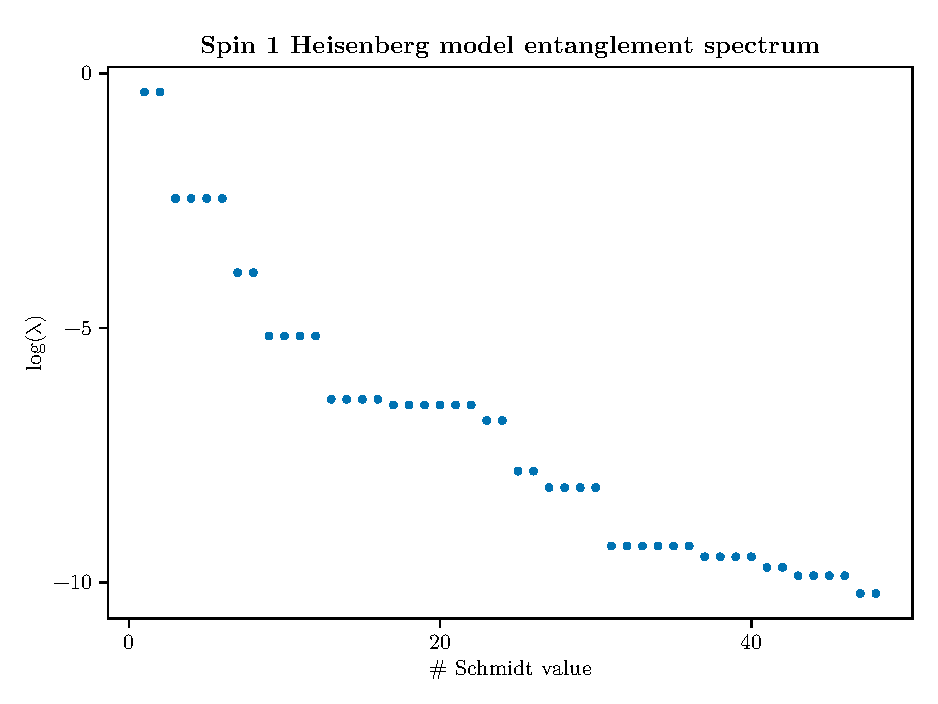
\includegraphics[width=0.7\linewidth]{plots/HeisenbergEntanglementSpectrum.pdf}
	\caption{The entanglement spectrum of the spin 1 Heisenberg model ground state in the thermodynamic limit with bond dimension 48. Created with MPSKit.jl~\cite{VanDamme}.}
	\label{fig:HeisenbergEntanglement}
\end{figure}

As anticipated above, a natural basis for the edge modes is given by the virtual degrees of freedom of the MPS ground state near the boundaries. Indeed, a uniform MPS on open boundary conditions,
\begin{equation}
	\ket{\Psi[A]} = \sum_{\{i_j\}} (A^{i_1}A^{i_2}\cdots A^{i_N})_{\alpha\beta} \ \ket{i_1,i_2,\dots,i_N},
\end{equation}
corresponds to $\chi^2$ states $\ket{\Psi[A], \alpha,\beta}$ that have the same energy for the parent Hamiltonian. Naively, we would thus count $\chi^2$ ground states on the open chain, but some of these modes can be gapped out by turning on additional terms in the Hamiltonian. However, as long as these additional terms respect the symmetry, a certain amount of degeneracy is persistent; these edge modes transform under the symmetry action according to
\begin{equation}
	U(g)^{\otimes N}\ket{\Psi[A],\alpha,\beta} = \sum_{\alpha',\beta'} (X_g)_{\alpha\alpha'} (\bar X_g)_{\beta\beta'}\,\,\ket{\Psi[A],\alpha',\beta'},
\end{equation}
so that at least a two-fold degeneracy persists.

\bigskip\noindent This concludes phase classification in the one-dimensional setting where the symmetry acts via a unitary (tensor product) group representation. To summarise, phases are classified by pairs $(H,[\psi])$ where $H\subseteq G$ is a subgroup up to conjugacy and $[\psi]$ is a class taking values in $H^2(H,\rU(1))$~\cite{Chen2010,Schuch2011}.

Remarkably, these data also classify (indecomposable) \emph{module categories} $\mc R(H,\psi)$ over the \emph{fusion category} $\Vect_G$~\cite{Ostrik2001,Etingof2015}. \emph{Simple objects} of the corresponding module category are labelled by cosets $\{r_1H,r_2H,\dots\}$ and $\mc R(H,\psi)$ carries a natural $\Vect_G$ action induced by $g\act rH:= (gr)H$. This observation suggests the physical interpretation where the gapped ground states are identified with the simple objects, and the action $\act$ with the action of the on-site $G$ symmetry on the ground state subspace. 

This observation is more than a formal analogy and is the first indication of a correspondence between module categories and gapped phases of matter. The \emph{generalised Landau paradigm}, the subject of \cref{sec:GenLandau}, stipulates that this correspondence persists to one-dimensional (lattice) models with a symmetry described by a generic fusion category $\mc C$~\cite{Thorngren2019,GarreRubio2022,Bhardwaj2023,Lootens2024}. More precisely, it states that the different gapped phases are given by the different module categories $\mc P$ over $\mc C$, with the simple objects labelling the ground states and the \emph{module action} describing the symmetry action on them.
\chapter{Non-chiral topological order: string-nets and categories}\label{ch:topo}
In the previous chapter we outlined the classification of one-dimensional bosonic gapped phases of matter, which required the presence of a symmetry to protect a non-trivial phase. This radically changes in one dimension higher since even in the absence of any symmetries, gapped \emph{intrinsic topological phases} arise. These phases are characterised by a \emph{robust ground state degeneracy} that depends only on the topology of the underlying spatial manifold, \emph{anyonic} quasiparticle excitations and in some cases \emph{edge modes}.

In this chapter we focus on \emph{non-chiral} topological phases that admit \emph{gapped boundary conditions}. It is believed that these phases are fully characterised by their anyon content, corresponding fusion rules and braiding statistics. This brings us into the realm of \emph{category theory} since these data are naturally encapsulated in a \emph{modular fusion category}, specifically the \emph{Drinfeld} or \emph{monoidal centre} $\mc Z(\mc D)$ of a generically non-braided \emph{input} fusion category $\mc D$.

Importantly, every such topological order admits a lattice realisation directly in terms of this input $\mc D$. This is precisely the \emph{Levin-Wen string-net condensation model} that provides a frustration-free Hamiltonian whose torus ground state sectors and excitation spectrum exactly reproduce $\mc Z(\mc D)$. From the point-of-view of tensor networks, these string-net ground states admit particularly elegant PEPS representations characterised by the existence of MPO symmetries that live purely on the \emph{virtual} level, form a representation of a \emph{Morita equivalent} fusion category $\mc C$ and that can be continuously deformed through the lattice. Consequently, these MPO symmetries survive small physical perturbations and characterise the long-range entanglement structure.

\bigskip\noindent In this chapter, we review the string-net models and their PEPS representations. Significant attention is devoted to the classification and construction of their gapped boundaries. Beyond being interesting in their own right, the data characterising the gapped boundaries also classify \emph{gapped phases} of the string-net boundary Hamiltonians that inherit the (non-invertible) symmetries of the bulk topological order. This is the content of the \emph{generalised Landau paradigm} and is treated in the next chapter.
\section{Fusion categories for topological orders}
The description of non-chiral topological orders and their realisation in terms of string-net models requires the language of \emph{fusion categories} and \emph{modular fusion categories}.  Whereas the former is used to define the microscopic Hilbert space and Hamiltonian of the string-net models, the exchange statistics of the anyonic excitations are described by the \emph{non-degenerate}, \emph{modular}, \emph{braiding} encapsulated in the latter.

In what follows we will provide the necessary aspects of (braided) fusion categories, and thereby introduce their \emph{graphical calculus}. We invite the reader to consult the literature for a more precise and more complete technical treatment of these topics~\cite{Etingof2002,Kitaev2005a,Etingof2015,Beer2018}.

\bigskip\noindent It should be kept in mind that even though fusion categories are strictly richer structures than finite groups and their representation theory, they may in fact be regarded as a natural generalisation of both. Indeed, much of the structure of a fusion category can be understood as the categorical counterpart of familiar concepts from group and representation theory, a perspective that we illustrate in detail below. As a result, fusion categories provide a unified framework in which conventional symmetries encoded in groups and \emph{topological}, \emph{generalised} symmetries can be treated on equal footing.
\subsection{Algebraic structure of fusion categories}
\subsubsection{Simple objects and fusion}
Succinctly, a \emph{unitary fusion (1-)category} (UFC) $\mc C$ consists of a collection of objects $\ob(\mc C)$ to which we will refer as \emph{topological defects}, \emph{topological lines}, \emph{sectors} or \emph{charges}, depending on the context. Every $X\in\ob(\mc C)$ admits a decomposition as a direct sum of finitely many \emph{simple objects} $\mc I_\mc C=\{X_i\}_i$, i.e.:
\begin{equation}
	X = \bigoplus_{X'\in\mc I_\mc C} N_{X}^{X'} X',
\end{equation}
for non-negative integers $N_{X}^{X'}$ counting the multiplicity of each direct summand. The decomposition is unique for every object $X$, up to a permutation of the factors. The set $\ob(\mc C)$ is endowed with a \emph{monoidal} or \emph{tensor product} $\otimes: \mc C\times\mc C\rightarrow\mc C$ encoding the \emph{fusion} of defects. We will express this product in terms of an integer rank-3 tensor $N$ via:
\begin{equation}\label{eq:FusionRule}
	X_1 \otimes X_2 = \bigoplus_{X_3\in\mc I_\mc C} N_{X_1X_2}^{X_3} X_3,
\end{equation}
for simple objects $X_1, X_2$. These fusion rules are \emph{associative} so that for any four simple objects we have that $\sum_X N_{X_1X_2}^X N_{XX_3}^{X_4} = \sum_X N_{X_1X}^{X_4} N_{X_2X_3}^X$. Generically $N_{X_1X_2}^{X_3}\neq N_{X_2X_1}^{X_3}$. Moreover, since the tensor product $\otimes$ distributes over the direct sum $\oplus$, the product of all objects is defined fully by \cref{eq:FusionRule}. Among the simple objects, there exists a unique \emph{monoidal unit} notated as $\mbb 1_\mc C$ or simply $\mbb 1$ that satisfies $\mbb 1\otimes X= X\otimes\mbb 1= X$, $\forall X\in\ob(\mc C)$. To every object $X$ there corresponds a unique \emph{dual} $X^*$ characterised by $N_{XX^*}^{\mbb 1} = 1$.

Below, we also make use of the \emph{quantum dimensions} $d_X$ of the simple objects which are completely specified by
\begin{equation}
	\begin{split}
		d_X &> 0, \\
		d_{X_1}\, d_{X_2} &= \sum_{X_3\in\mc I_\mc C} N_{X_1X_2}^{X_3} \, d_{X_3}.
	\end{split}
\end{equation}
In particular we have $d_\mbb 1=1$ and $d_{X}=d_{X^*}$, for all $X\in\ob(\mc C)$. Also, the quantum dimensions are additive over the direct sum, so that $d_X=\sum_{X'\in\mc I_\mc C} N_{X}^{X'} d_{X'}$ for any $X\in\ob(\mc C)$.
\subsubsection{Graphical calculus}
The different ways in which simple objects $X_1$ and $X_2$ can fuse to $X_3$ is captured by the \emph{fusion space} $\mc C(X_1\otimes X_2,X_3)\simeq\mbb C^{N_{X_1X_2}^{X_3}}$ for which we use the shorthand $\mc C^{X_1X_2}_{X_3}$. In category theoretic parlance, this Hilbert space for every triple of objects is referred to as \emph{Hom}, \emph{fusion} or \emph{junction space}. Notably, for simple objects $X_1,X_2$ we have $\mc C(X_1,X_2) = \delta_{X_1,X_2}\mbb C$. Basis vectors are notated as $|X_1X_2X_3; i \ra \in \mc C^{X_1X_2}_{X_3}$ with $i=1,2,\dots,N_{X_1X_2}^{X_3}$. These vectors and their duals can be depicted in terms of strings diagrams as follows:
\begin{equation}
	|X_1X_2X_3; i \ra \equiv \inputtikz{FusionVertex}\, , \quad \la X_1X_2X_3; i | \equiv \inputtikz{SplittingVertex}\, .
\end{equation}
Here and below, all string diagrams are implicitly oriented downwards. We adopt a normalisation of these basis vectors such that the following graphical identity holds:
\begin{equation}\label{eq:BubblePop}
	\inputtikz{BubblePop1} = \delta_{X_3,X_3'} \delta_{i,j} \, \sqrt{\frac{d_{X_1}d_{X_2}}{d_{X_3}}} \, \inputtikz{BubblePop2}\, .
\end{equation}
Note that the basis vectors are not normalised to one. Indeed the inner product of basis vectors can be depicted as:
\begin{equation}
	\la X_1X_2X_3; i | X_1X_2X_3; j \ra = \inputtikz{VertexNorm} = \delta_{i,j} \sqrt{d_{X_1}d_{X_2}d_{X_3}},
\end{equation}
which for the particular case of $X_1=\mbb 1$, $X_2=X_3\equiv X$ specialises to
\begin{equation}\label{eq:qdim}
	\inputtikz{qdim} = d_X.
\end{equation}
This normalisation is referred to as the \emph{isotopy invariant} normalisation convention, but other conventions are used throughout the literature~\cite{Kitaev2005a}. In this normalisation, the completeness of the basis then boils down to:
\begin{equation}\label{eq:ResId}
	\inputtikz{ResId1} = \sum_{X_3,i} \sqrt{\frac{d_{X_3}}{d_{X_1}d_{X_2}}} \,\, \inputtikz{ResId2}.
\end{equation}
Consider now the fusion of three simple objects. In virtue of the associativity of the fusion rules, the associated Hom space capturing the fusion of these three objects decomposes in two distinct but isomorphic ways as follows:
\begin{equation}
	\mc C^{X_1X_2X_3}_{X_4} \simeq \bigoplus_{X_5} \mc C^{X_1X_2}_{X_5} \otimes \mc C^{X_5X_3}_{X_4} \simeq \bigoplus_{X_6} \mc C^{X_1X_6}_{X_4} \otimes \mc C^{X_2X_3}_{X_6},
\end{equation}
for all simples $X_4$ appearing in the decomposition of $X_1\otimes X_2 \otimes X_3$. The unitary isomorphism between both decompositions is given by the \emph{$F$-symbol} or \emph{associator}\footnote{The $F$-symbol has an interpretation as the complex number that $\mc C$ assigns to the planar projection of a tetrahedron whose edges are decorated by objects in $\ob(\mc C)$ and vertices decorated by junction spaces. In what follows we will assume the $F$-symbol to be independent of the chosen projection. This property is known as \emph{tetrahedral symmetry}, and not every UFC satisfies this. We refer to ref.~\cite{Hahn2020} for the generalisation of the string-net construction to fusion categories that do not enjoy this symmetry.} $F^{X_1X_2X_3}$ and its matrix components are conveniently depicted in terms of the \emph{F-move}
\begin{equation}\label{eq:Fmove}
	\inputtikz{Fmove1} = \sum_{X_6,k,l} \big(F^{X_1X_2X_3}_{X_4}\big)_{X_5,ij}^{X_6,kl} \inputtikz{Fmove2}.
\end{equation}
An $F$-symbol is set to zero when not all of the involved fusion rules are fulfilled. Crucially, they also satisfy a \emph{consistency equation} or \emph{coherence axiom} colloquially known as the \emph{pentagon equation} which in full reads:
\begin{equation}\label{eq:pent}
	\begin{gathered}
		\sum_o \left(F^{X_6X_3X_4}_{X_5}\right)^{X_8,no}_{X_7,lm}
		\left(F^{X_1X_2X_8}_{X_5}\right)^{X_9,pq}_{X_6,ko} \\
		= \sum_{X_{10},rst}
		\left(F^{X_1X_2X_3}_{X_7}\right)^{j,rs}_{X_6,kl}
		\left(F^{X_1X_{10}X_4}_{X_5}\right)^{X_9,tq}_{X_7,sm}
		\left(F^{X_2X_3X_4}_{X_9}\right)^{X_8,np}_{X_{10},rt}
	\end{gathered}.
\end{equation}
In virtue of \emph{Ocneanu rigidity}, the number of solutions to the pentagon equation, up to basis transformations of the Hom spaces, is finite for any valid set of fusion rules.
\subsection{Examples}
Before proceeding, let us provide a few paradigmatic examples of these rather abstract definitions.
\subsubsection{Finite group symmetry: $\Vect_G^\omega$} Let $G$ be a finite group. The fusion category $\Vect_G$ is the category of (complex finite-dimensional) $G$-graded vector spaces. Its fusion rules are completely defined by
\begin{equation}
	(V\otimes W)_g = \bigoplus_{hk=g} V_h \otimes W_k
\end{equation}
$\forall g,h,k\in G$, where $V_g$ stands for the $g$-graded component of $V$. Representative simple objects of $\Vect_G$ are the one-dimensional vector spaces $\{\mbb C_g\}_{g\in G}$ and are thus in bijection with the group elements of $G$. Abusing notation, they are sometimes simply denoted by $g\equiv\mbb C_g$. The non-vanishing $F$-symbols are all equal to one when all fusion rules are fulfilled. Whenever $G$ possesses a non-trivial \emph{third cohomology group} $H^3(G,\rU(1))$, a non-trivial 3-cocycle $\omega$ can be used to construct $\Vect_G^\omega$. This fusion category is constructed analogously to $\Vect_G$ where now the non-zero components of the $F$-symbols evaluate to $\omega$. In that case, the pentagon equation is equivalent to the 3-cocycle condition satisfied by $\omega$.
\subsubsection{Finite group representations: $\Rep(G)$} Intimately connected to $\Vect_G$ is the category $\Rep(G)$, again for a finite group $G$.\footnote{For all $G$, $\Vect_G$ and $\Rep(G)$ are \emph{Morita equivalent}, as explained below. This means that their Drinfeld centres $\mc Z(\Vect_G)$ and $\mc Z(\Rep(G))$ are equivalent as braided fusion categories.} This category encodes as objects the (unitary finite-dimensional) representations of $G$. Representative \emph{irreducible} representations then constitute the simple objects and their fusion is given by the usual tensor product of $G$-representations. It can then be deduced that the 6-j symbols are in this case the matrix coefficients of the monoidal associator.
\subsubsection{The Fibonacci fusion category: $\Fib$} The \emph{Fibonacci} UFC $\Fib$ consists of two objects labelled by $\{\mbb 1, \tau\}$ whose only non-trivial fusion rule reads $\tau\otimes\tau=\mbb 1\oplus \tau$. The quantum dimension of $\tau$ is easily found to be the golden ratio $d_\tau = \varphi = \frac{1+\sqrt 5}{2}=1.618\dots$, indicative of the fact that $\Fib$ is not realised as the representation category of any finite group as this would require $d_\tau$ to be a non-negative integer. The non-trivial $F$-symbols read:
\begin{equation}
	F^{\tau\tau\tau}_{\tau} =
	\frac{1}{\varphi}
	\begin{pmatrix}
		1 & \sqrt{\varphi} \\
		\sqrt{\varphi} & -1
	\end{pmatrix}.
\end{equation}

\bigskip\noindent As anticipated above, we come to the intermediate conclusion that fusion categories provide a framework that not only unifies finite group and representation theory --- as exemplified by the fusion categories $\Vect_G$ and $\Rep(G)$ --- but also extends it --- e.g. in the form of the Fibonacci category. As a guide to the reader, we compactly summarise this in  \cref{tab:categorical}:
\vfill
\begin{table}[h]
	\centering
	\renewcommand{\arraystretch}{2}
	\begin{tabular}{|>{\centering\arraybackslash}p{4cm}
			|>{\centering\arraybackslash}p{4cm}
			|>{\centering\arraybackslash}p{4cm}|}
		\hline
		$\Vect_G$ & $\Rep(G)$ & Categorical notion \\
		\hline
		$G$-graded vector spaces $V, W, U,\dots$
		& $G$-representations $(V_i, \rho_i)$
		& Objects $\ob(\mc C)$ \\
		\hline
		Grading-preserving linear maps $\phi: V \to W$ 
		& Intertwiners $f \circ \rho_1 = \rho_2 \circ f$ 
		& Hom spaces $\mc C(X,X')$ \\
		\hline
		$\Vect_G(\mbb C_{g_1}, \mbb C_{g_2}) = \delta_{g_1, g_2}\, \mbb C$
		& $\Rep(G)(\alpha_i, \alpha_j) = \delta_{i,j}\,\mbb C$, w/ $\alpha_i,\alpha_j$ irreps \;(Schur)
		& Simple objects $\mc C(X_1,X_2) = \delta_{X_1,X_2}\,\mbb C$ \\
		\hline
		$(V \otimes W)_g = \bigoplus_{hk=g} V_h \otimes W_k$
		& $\alpha_i \otimes \alpha_j \simeq \bigoplus_k N_{ij}^k\,\alpha_k$
		& Monoidal product \& fusion rules \\
		\hline
		$\mbb C_1 \otimes V \simeq V \simeq V \otimes\, \mbb C_1$
		& $\ub 1 \otimes \rho \simeq \rho \simeq \rho \otimes \ub 1$, w/
		$\ub 1$ the trivial irrep
		& Monoidal unit $\mbb 1$ \\
		\hline
		$\mbb C_g \otimes \mbb C_{g^{-1}} \simeq \mbb C_1$
		& $\alpha \otimes \alpha^* \ni \ub 1$
		& Dual object \\
		\hline
		$F: (V \otimes W) \otimes U \xrightarrow{\sim} V \otimes (W \otimes U)$, w/ $F$ trivial
		& $F: (\alpha_1 \otimes \alpha_2) \otimes \alpha_3 \xrightarrow{\sim} \alpha_1 \otimes (\alpha_2 \otimes \alpha_3)$, w/ $F$ the 6-j symbols
		& $F$-symbol (Monoidal associator) \\
		\hline
	\end{tabular}
	\caption{Comparison of $\Vect_G$, $\Rep(G)$, and their categorical generalisations.}
	\label{tab:categorical}
\end{table}
\vfill
\clearpage
\subsection{Braiding}
Finally, we introduce the \emph{braiding} of two defects diagrammatically as:
\begin{equation}\label{eq:Braid}
	R^{X_1X_2} := \inputtikz{Braid_1}, \qquad \big(R^{X_1X_2}\big)^{-1} := \inputtikz{Braid_2}.
\end{equation}
Typically, $R^{X_1X_2}\circ R^{X_2X_1}\neq {\rm id}_{X_1\otimes X_2}$ so that in the graphical calculus one should keep track of the distinction between \emph{over} and \emph{underbraiding} of the strands. Categories for which $R^{X_1X_2}\circ R^{X_2X_1}$ is the identity map on $X_1\otimes X_2$, are called \emph{symmetric}.

The components of the braiding \cref{eq:Braid} in our choice of basis then give rise to the unitary \emph{R-matrix} defined via:
\begin{equation}\label{eq:RMove}
	\inputtikz{RMove1} = \sum_j \big( R^{X_1X_2}_{X_3}\big)_{ij} \inputtikz{RMove2}.
\end{equation}
The braiding is required to satisfy a consistency equation called the \emph{hexagon equation} that also involves the $F$-symbols. A fusion category is called \emph{braided} or \emph{pre-modular} when it is endowed with a braiding that satisfies the hexagon axiom. For any braided fusion category we then define the \emph{topological S-matrix} $S_{X_1,X_2}$ via the amplitudes
\begin{equation}\label{eq:Smat}
	\begin{gathered}
		S_{X_1,X_2} := \frac{1}{\Dim\,\mc C} \inputtikz{Smat} \\
		= \frac{1}{\Dim\,\mc C} \sum_{X_3} N_{X_1X_2}^{X_3} d_{X_3} {\rm Tr}\big( R^{X_1X_2}_{X_3}R^{X_2X_1}_{X_3}\big),
	\end{gathered}
\end{equation}
where we have defined the \emph{total quantum dimension} or \emph{Frobenius-Perron dimension of $\mc C$} as $\Dim\,\mc C := \sum_{X\in\mc I_\mc C} d_X^2$. Physically, the amplitudes \cref{eq:Smat} correspond to an interferometry process in which two defects $X_1$ and $X_2$ are created from the vacuum, exchanged and annihilated again. Notably, if for every $X_1\neq\mbb 1$ there exists at least one $X_2\neq\mbb 1$ such that their double-braiding $R^{X_1X_2}\circ R^{X_2X_1}$ is non-trivial, the S-matrix is non-degenerate~\cite[Cor. 2.16]{Mueger2003}. Physically, this means that every non-trivial defect can be distinguished from the vacuum by double-braiding it with a suitable probe defect. This is called the \emph{principle of remote detectability}~\cite{Levin2013,Kong2014}. This motivates the definition of a \emph{modular} fusion category, which is a pre-modular fusion category with non-degenerate S-matrix.
\subsection{Examples}
\subsubsection{Finite group symmetry: $\Vect_G^\omega$} Evidently, $\Vect_G$ only admits a braiding if $G$ is abelian. In that case the braiding is provided by a choice of \emph{bilinear form} $b$, meaning a map $b:G\times G\to \rU(1)$ satisfying
\begin{equation}
	\begin{split}
		b(g_1,g_3)\cdot b(g_2,g_3) &= b(g_1g_2,g_3), \\
		b(g_1,g_2)\cdot b(g_1,g_3) &= b(g_1,g_2g_3),
	\end{split}
\end{equation}
for all $g_1,g_2,g_3\in G$. When the associator belongs to a non-trivial class $[\omega]\in H^3(G,\rU(1))$,  admissible associator-braiding pairs are in one-to-one correspondence with the elements of the \emph{abelian} cohomology group $H^3_{\rm ab}(G,\rU(1))$. We refer to the relevant literature for a precise definition and construction of the braiding~\cite{Etingof2015}.
\subsubsection{Finite group representations: $\Rep(G)$} The category $\Rep(G)$ admits a symmetric braiding that amounts to the transposition of representation spaces, i.e. $R:V_1\otimes V_2 \to V_2\otimes V_1$ for $(V_1,\rho_1)$, $(V_2,\rho_2)$ in $\ob(\Rep(G))$.
\subsubsection{The Fibonacci fusion category: $\Fib$} The Fibonacci category admits a \emph{modular} braiding. Indeed, its $S$-matrix
\begin{equation}
	S =
	\frac{1}{\sqrt{2+\varphi}}
	\begin{pmatrix}
		1 & \varphi \\
		\varphi & -1
	\end{pmatrix},
\end{equation}
is non-degenerate~\cite{Rowell2007}.
\section{String-net models}\label{sec:SNModels}
\subsection{Hilbert space and Hamiltonian}
Let $\mc D$ be a UFC whose objects we denote by $\{Y\}$, and $\Lambda$ be an \emph{oriented trivalent lattice} $\Lambda$ without boundary. The microscopic string-net Hilbert space on $\Lambda$ is constructed from the \emph{input} $\mc D$ as follows~\cite{Levin2004,Kirillov2011}. A basis state corresponds to an assignment, or \emph{$\mc D$-colouring}~\cite{Kirillov2011}, of simple objects $Y\in\mc I_\mc D$ to all the edges $\msf E(\Lambda)$, with the requirement that the fusion rules are satisfied on all vertices $\msf V(\Lambda)$. Conventionally, reversing the orientation of an edge $\msf e\to-\msf e$ amounts to taking the dual object on that edge. Then, to every vertex with adjacent edges labelled $Y_1,Y_2,Y_3$ the junction space $\mc C(Y_1\otimes Y_2,Y_3)$ is attached. In what follows we specialise to the \emph{hexagonal lattice}. On it,  the Hilbert space $\mc H_\mc D(\Lambda)$ is thus defined as:
\begin{equation}
	\mc H_{\mc D}(\Lambda)  := {\rm Span}_\mbb C \Bigg\{ \quad \inputtikz{SNSpace} \quad \big| \, \{Y\}, \{i\}\Bigg\},
\end{equation}
where it is understood that the picture extends over the entire lattice. In correspondence with our graphical calculus, we also assume all edges to be oriented downwards.

\bigskip\noindent On every plaquette $\msf p\in\msf P(\Lambda)$ and for every $Y\in\mc I_\mc D$ we subsequently define a local operator $B_\msf p^Y$. This operator admits a particularly intuitive definition as inserting a \emph{non-contractible} counter-clockwise loop labelled by the simple object $Y$ in the plaquette and fusing it into the physical lattice with local applications of the resolution of the identity $F$-moves, and normalisation of the basis vectors \cref{eq:ResId,eq:Fmove,eq:BubblePop}. In order for this to be consistent with our graphical calculus, and in particular the quantum dimension relation \cref{eq:qdim}, we should therefore think of the underlying manifold as being \emph{punctured} in the interior of every plaquette in $\msf P(\Lambda)$. Schematically, the action can therefore be depicted as:
\begin{gather}
	B_\msf p^Y \cdot \ket{\Psi} =
	\inputtikz{SNPlaquette_1}
	\overset{\eqref{eq:ResId}}{\mapsto}
	\sum \{d\} \inputtikz{SNPlaquette_2} \\
	\overset{\substack{\eqref{eq:Fmove} \\ \eqref{eq:BubblePop}}}{\mapsto}
	\sum \{d\}\{F\} \inputtikz{SNPlaquette_3}.
\end{gather}
Herein, we have for simplicity omitted all edge and vertex labels; $\{d\}$ and $\{F\}$ are placeholders for the quantum dimensions and $F$-symbols obtained via repeated use of the aforementioned identities. We refer to \cite{Levin2004} for an explicit computation of these matrix elements. We can also infer from application of our graphical calculus that these plaquette operators form a representation of the fusion rules, viz.:
\begin{equation}\label{eq:ProdBp}
	B_\msf p^{Y_1}\cdot B_\msf p^{Y_2} = \sum_{Y_3} N_{Y_1Y_2}^{Y_3} B_\msf p^{Y_3}.
\end{equation}
With these plaquette operators at our disposal, the local Hamiltonian terms are constructed as:
\begin{equation}\label{eq:BpD}
	B_\msf p^\mc D = \sum_{Y\in\mc I_\mc D} \frac{d_Y}{\Dim\mc D} B_\msf p^Y =: \, \inputtikz{SNBp} \,\, .
\end{equation}
From combining \cref{eq:ProdBp} with the identity
\begin{equation}
	d_Y\, \Dim\mc D = \sum_{Y_1, Y_2} N_{Y_1Y_2}^Y d_{Y_1} d_{Y_2},
\end{equation}
it directly follows that $B_\msf p^\mc D$ is an idempotent for every $\msf p\in\msf P(\Lambda)$, i.e. $B_\msf p^\mc D \cdot B_\msf p^\mc D=B_\msf p^\mc D$, $\forall\msf p$. Commutation of plaquette operators $B_\msf p^\mc D$ and $B_{\msf p'\neq\msf p}^\mc D$ is immediate when $\msf p$ and $\msf p'$ are far separated. When $\msf p$ and $\msf p'$ share an edge this follows from comparing the matrix elements of both application orders and invoking the pentagon equation \cref{eq:pent} on their matrix elements. The string-net Hamiltonian is then finally given by
\begin{equation}
	H_{\mc D}(\Lambda) = -\sum_{\msf p\in\msf P(\Lambda)} B_\msf p^\mc D.
\end{equation}
Remark that a ground state of $H_{\mc D}(\Lambda)$ can be constructed by acting with the ground state projector $\prod_\msf p B_\msf p^\mc D$ --- which is well-defined since all $B_\msf p^\mc D$'s commute --- on a generic string-net state in $\mc H_\mc D(\Lambda)$. This is exactly the approach taken in \cref{sec:SNPEPS} to write down the ground state PEPS representations.

Importantly, the ground state subspace is one-dimensional when the underlying lattice has the topology of a two-sphere~\cite{Kirillov2011}. However, on the two-torus the ground space is degenerate, and the degeneracy does not depend on the system size. Due to the absence of any global symmetry, this degeneracy cannot be traced back to ordinary symmetry breaking as discussed in \cref{sec:1Dphases}. Rather, the ground state degeneracy can be understood as the breaking of a more general type of symmetry whose operators are supported on oriented \emph{freely deformable} loops $\ell$ on the lattice. Such operators constitute an example of a \emph{global 1-form} symmetry~\cite{Nussinov2009,Gaiotto2014,McGreevy2022}.\footnote{In general, a $(D+1)$-dimensional quantum theory is said to host a \emph{global $p$-form symmetry} if there exist symmetry operators supported on freely-deformable closed submanifolds of \emph{codimension} $p$ with respect to the spatial dimension~\cite{Gaiotto2014,McGreevy2022}.}

These loop operators, and their multiplication rules, are encoded in the \emph{monoidal} or \emph{Drinfeld centre} $\mc Z(\mc D)$ of $\mc D$.
\subsection{Loop operators and ground states}\label{sec:SNGSs}
Formally, the centre $\mc Z(\mc D)$ is a unitary fusion category whose simple objects are pairs $(Z,\gamma_{Z,\bullet})$ where $Z$ is a (generically non-simple) object in $\mc D$ and $\gamma_{Z,\bullet}$ is a natural isomorphism, called the \emph{half-braiding}. Its matrix elements can be expressed graphically as
\begin{equation}\label{eq:HalfBraid}
	\inputtikz{HalfBraid1} = \sum_{Y_2} \sum_{i,j} \big( \Gamma^{Y_1Z}_{Y_2}\big)_{ij} \inputtikz{HalfBraid2} \, ,
\end{equation}
$\forall Y_1\in\mc I_\mc D$. The half-braiding satisfies a hexagon consistency axiom involving the associator of $\mc D$. Consequently, $\mc Z(\mc D)$ can be endowed with a \emph{modular} braiding, defined directly in terms of $\gamma_{Z,\bullet}$~\cite{Mueger2001}. Naturality of $\gamma_{Z,\bullet}$ implies the following graphical equality:
\begin{equation}\label{eq:SNPT}
	\inputtikz{SNPullingThrough_3} = \inputtikz{SNPullingThrough_4} \, ,
\end{equation}
for all admissible junctions $| Y_1Y_2Y_3, i \ra$. Below, we often abuse notation and write simply $Z$ instead of $(Z,\gamma_{Z,\bullet})$.

In order to define the action of a loop labelled by $(Z,\gamma_{Z,\bullet})$ on a state, one proceeds in a similar fashion as in the definition of the plaquette operators. One inserts the object $Z$ along the path $\ell$, and locally fuses it into the physical lattice, thereby making use of the half-braiding \cref{eq:HalfBraid} at every crossing with the physical lattice and the usual local recoupling identities \cref{eq:ResId,eq:Fmove,eq:BubblePop}. An illustration of such a loop is:
\begin{equation}
	\inputtikz{SNTopoLine1}\,\,.
\end{equation}
Although drawn as a line, it should be remarked that these operators act (diagonally) on edges adjacent to their path and are therefore more precisely interpreted as \emph{ribbon operators} with a finite width. These coincide with those introduced by Kitaev in ref.~\cite{Kitaev1997} and Levin and Wen in ref.~\cite{Levin2004}, see also refs.~\cite{Beigi2010,Dauphinais2018}.

The \emph{topological} nature of the loop operator follows directly from the naturality condition \cref{eq:SNPT}, which ensures that $Z$ can slide freely across any junction of the physical lattice without altering the resulting operator. Note that this topological invariance also accounts for the commutativity with the Hamiltonian. When a loop and a plaquette operator have disjoint support, they commute trivially. When they have overlapping support, one can deform the loop away from the plaquette before acting with the latter, and subsequently restore the path of the loop, so that the combined action remains unchanged.

\bigskip\noindent Provided a reference string-net ground state one can construct a complete basis of torus ground states by acting with all simple loop operators $(Z,\gamma_{Z,\bullet})\in\mc I_{\mc Z(\mc D)}$ along a non-contractible cycle of the torus. We therefore conclude that the torus ground state degeneracy is given by $|\mc I_{\mc Z(\mc D)}|$. This also implies that orthogonal ground states are locally indistinguishable, as the precise location of the $Z$-loop can be continuously deformed and is thus invisible for any local operator. Acting on the other hand with loop operators along the perpendicular non-contractible cycle provides a different set of ground states that are related to the former via the unitary basis transformation given by the $S$-matrix of $\mc Z(\mc D)$ defined in \cref{eq:Smat}~\cite{Pfeifer2010}.
\newpage
\subsection{String operators and excited states}\label{sec:LoopsExcited}
Similar to the construction of ground states via loop operators, excited states are constructed by acting on the ground states with \emph{open} string operators, also labelled by objects $(Z,\gamma_{Z,\bullet})\in\mc I_{\mc Z(\mc D)}$. Such a state corresponds to an \emph{$(Z,Z^*)$-anyon--anti-anyon pair}, and schematically can be depicted as
\begin{equation}\label{eq:AnyonPairStrings}
	\inputtikz{AnyonPairStrings}\,\,.
\end{equation}
In this sense, the different ground states constructed in \cref{sec:SNGSs} can be understood as the result of creating a $(Z,Z^*)$-pair from a reference ground state, dragging one of the anyons around a non-contractible cycle before annihilating the pair.

\bigskip\noindent Importantly, note that in fusing the open string in \cref{eq:AnyonPairStrings} to the physical lattice, one is in general left with dangling vertical edges on the plaquettes on which the string starts and terminates, if $Z$ decomposes as a non-trivial object of $\mc D$. In that case the obtained state does not belong to the string-net Hilbert space, and the corresponding anyons are said to possess a non-trivial \emph{charge}. Accommodating this type of excitations naturally leads us to consider the \emph{extended} string-net models, first introduced in ref.~\cite{Hu2015}. In this framework, the string-net Hilbert space is extended with extra open strands or \emph{tails}, one for every vertex of the original lattice. Consequently, all anyonic excitations, also those with a non-trivial charge, can be considered without the need to leave the Hilbert space or violate the $\mc D$ fusion rules. Concretely, on the hexagonal lattice, the extended Hilbert space is defined as:
\begin{equation}
	\mc H_{\mc D}^{\rm Ext.}(\Lambda)  := {\rm Span}_\mbb C \Bigg\{ \quad \inputtikz{SNSpaceExtended} \quad \big| \, \{Y\}, \{i\}\Bigg\}\,.
\end{equation}
In this depiction, an identification between every tail and the closest vertex of the hexagonal lattice is assumed. The extended Hamiltonian consists of the plaquette terms which generalise those introduced in \cref{eq:BpD}, and are defined in detail in ref.~\cite{Hu2015}, and additionally \emph{vertex terms} $Q_\msf v^\mc D$ for every $\msf v\in\msf V$. These act by projecting the tail corresponding to $\msf v$ to the identity object. Concretely, locally:
\begin{equation}
	Q_\msf v^\mc D \,\, \Bigg| \inputtikz{SNextendedQ_1} \Bigg> = \delta_{Y,\mbb 1} \,\, \Bigg| \inputtikz{SNextendedQ_2} \Bigg>\,\,.
\end{equation}
Collecting everything, the extended string-net Hamiltonian is of the form
\begin{equation}
	H_{\mc D}^{\rm Ext.}(\Lambda) = -\sum_{\msf p\in\msf P(\Lambda)} B_\msf p^\mc D -\sum_{\msf v\in\msf V(\Lambda)} Q_\msf v^\mc D .
\end{equation}

Notably, in the subspace defined by $Q^\mc D_\msf v=1$, $\forall\msf v\in\msf V$, the extended string-net model coincides with the original Levin-Wen string-net.

\bigskip\noindent At this point we will not attempt to describe in further detail the action of the loop operators, the explicit ground states or excited states. Rather, we demonstrate in \cref{sec:SNPEPS} the construction of distinct PEPS representations of string-net ground states. The upshot of the tensor network approach is that a complete basis of torus ground states can be constructed by inserting a network of \emph{matrix product operators} living purely on the \emph{virtual level} of the PEPS. The network to insert corresponds concretely to \emph{central idempotents} of the \emph{tube algebra}. In fact, the representation theory of the tube algebra is often used to construct an explicit realisation of the Drinfeld centre. This description of the torus ground states is significantly simpler than working with the ribbon operators. Also, crucially, since the MPOs live on the virtual level, they survive physical perturbations and hence furnish a representation of the symmetries of the boundary Hamiltonians discussed in \cref{sec:dualities}. In a similar spirit, by introducing a new type of tensors whose support is specified by a central idempotent of the tube algebra, excited states also admit a PEPS representation.
\section{Gapped boundaries and domain walls}\label{sec:Bdry}
\subsection{Gapped boundaries} 
So far we have restricted our attention to the case of closed boundary conditions. As anticipated in the introduction, we can define string-net models with different types of open boundary conditions while preserving the gap. One choice of boundary is obtained by simply terminating the lattice, in which case the edge degrees of freedom are labelled by objects and junctions in $\mc D$. This demonstrates that every string-net model has at least one gapped boundary, to which we refer as the \emph{regular} or \emph{smooth} boundary condition, but depending on the input $\mc D$, other choices might be possible~\cite{Kitaev2011,Kong2015}.

The boundary conditions that we will study momentarily are constructed in such a way that the bulk plaquette operators can be extended to the boundary degrees of freedom while retaining their mutual commutativity. Commutation of the plaquette operators follows, similar as in the bulk, from local relations involving the $F$-symbols of $\mc D$.

To this end, let us introduce a new set of labels $\mc I_\mc R = \{R_1,R_2,\dots\}$ for these boundary degrees of freedom, and an action of $\mc D$ on those labels implemented via $R_1\cat Y = \sum_{R_2\in\mc I_\mc R} N_{R_1Y}^{R_2}R_2$ so that vertices on the boundary host a new type of vector space with basis vectors $|R_1YR_2; i \ra$, $i=1,2,\dots,N_{R_1Y}^{R_2}$. Schematically, the lattice of the string-net states in the presence of such a boundary looks like:
\begin{equation}
	\inputtikz{SNSmoothBoundary}\,\,\, ,
\end{equation}
where we draw edges that carry labels in $\mc I_\mc R$ in {\color{BlueViolet}blue}. The type of Hom space can be inferred from the colour of the adjacent edges.
Similar as in the bulk we define a unitary isomorphism $\rF$, generically distinct from the earlier defined $F$-symbol, whose matrix entries are defined graphically in terms of an \emph{$\rF$-move}:
\begin{equation}\label{eq:ModFmove}
	\inputtikz{ModuleAssociator1} = \sum_{Y_3,ij} \big( \rF^{R_1Y_1Y_2}_{R_2} \big)^{Y_3,kl}_{R_3,ij} \,\, \inputtikz{ModuleAssociator2}.
\end{equation}
We refer to $\rF$ as the \emph{(right) module associator}, and explain this terminology below. We require the $\rF$-symbols to adhere to a consistency axiom involving the $F$-symbols of $\mc D$ that is of the form
\begin{equation}\label{eq:ModPent}
	\rF \, \rF = \sum F\, \rF \, \rF.
\end{equation}
Its explicit form is straightforward to derive and spelled out in many places, e.g. ref.~\cite{Lootens2020}. For later reference, let us also introduce quantum dimensions of objects in $\mc I_\mc R$ in the sense of refs.~\cite{Schaumann2012,Etingof2015} via:
\begin{equation}
	\begin{split}
		d_R &> 0 \\
		d_R\, d_Y &= \sum_{R'\in\mc I_R} N_{RY}^{R'} \, d_{R'},
	\end{split}
\end{equation}
for all $Y\in\mc I_\mc D$. The quantum dimensions $d_R$ are defined up to a global rescaling $d_R\mapsto \lambda \, d_R,\, \forall R\in\mc I_R$ for any $R$-independent positive real scalar $\lambda$. To fix it, we will adopt the canonical normalisation
\begin{equation}
	\Dim\mc R := \sum_{R\in\mc I_\mc R} d_R^2 = \sum_{Y\in\mc I_\mc D} d_Y^2 =: \Dim\mc D.
\end{equation}
In this normalisation, we have the resolution of the identity
\begin{equation}\label{eq:ModResId}
	\inputtikz{ModResId1} = \sum_{R',i} \sqrt{\frac{d_{R'}}{d_{R}d_{Y}}} \,\, \inputtikz{ModResId2},
\end{equation}
and the inner product
\begin{equation}\label{eq:ModBubblePop}
	\inputtikz{ModBubblePop1} = \delta_{R_2,R_2'} \delta_{i,j} \, \sqrt{\frac{d_{R_1}d_{Y}}{d_{R_2}}} \, \inputtikz{ModBubblePop2}\, .
\end{equation}
Succinctly, provided a unitary fusion category $\mc D$, the set of boundary labels $\mc I_\mc R$, together with the action $\cat$ and a solution to the pentagon equation \cref{eq:ModPent} form the defining data of a (unitary) \emph{right module category} $\mc R$ over $\mc D$~\cite{Ostrik2001,Etingof2015}. Similarly, we can define a \emph{left} module category to construct a gapped right boundary condition.

Notably, the \emph{opposite} of a \emph{right} module category $\mc R$ over $\mc D$, notated as $\mc R^{\rm op}$, is naturally a \emph{left} module category whose module action is defined as~\cite{Schaumann2012,Etingof2015}:
\begin{equation}
	Y \act^{\rm op} R := R \cat Y^*.
\end{equation}
The objects of this opposite module category can be interpreted as \emph{duals} of the objects in $\mc R$. This leads to the following graphical identity
\begin{equation}\label{eq:ModResId2}
	\inputtikz{ModResId3} = \sum_{Y,i} \sqrt{\frac{d_{Y}}{d_{R}d_{R^*}}} \,\, \inputtikz{ModResId4}.
\end{equation}

\bigskip\noindent For a generic choice of module category $\mc R$, the bulk plaquette operators are extended to plaquettes adjacent to the boundary by again inserting a punctured counter-clockwise loop labelled by $\bigoplus_{X\in\mc I_\mc D}\frac{d_X}{\Dim\,\mc D} X$ in the boundary plaquettes and absorbing them into the physical lattice by making use of the different resolutions of the identity, $F$-moves and normalisations eqs. \eqref{eq:ResId}, \eqref{eq:ModResId}, \eqref{eq:Fmove}, \eqref{eq:ModFmove}, \eqref{eq:BubblePop} and \eqref{eq:ModBubblePop}. It can be verified that the boundary plaquette operators commute with all the other Hamiltonian terms by virtue of \cref{eq:ModPent}, so that the Hamiltonian remains gapped near the boundary.
\subsection{Examples}
\subsubsection{The regular module category}
Every UFC $\mc D$ trivially defines a unitary indecomposable module category over itself. We will refer to this as the \emph{regular} module category. For this choice, the corresponding boundary condition is the smooth boundary condition.
\subsubsection{$\Vect_G$-module categories}\label{par:VecGMods} As anticipated in \cref{sec:1Dphases}, indecomposable (left) module categories over $\Vect_G$ are -- up to conjugacy -- specified by pairs $(H\subseteq G,\psi)$ where $[\psi]\in H^2(H,\rU(1))$. In what follows we write the corresponding module category as $\mc R(H, \psi)$.

The explicit construction of $\mc R(H, \psi)$ from the data $(H,\psi)$ is reviewed in detail in \cref{app:gauging}. Here we only recall a few key facts. For one, the object set $\mc I_\mc R$ is a transitive left $G$-set so that it can be identified with the cosets $G/H$ endowed with the canonical left $G$-action. The module associator $\lF$ can then be constructed from the cocycle $\psi$ by making use of Shapiro's isomorphism between the cohomology groups $H^2(H,\rU(1)) \simeq H^2(G,{\rm Fun}(G/H,\rU(1)))$, where ${\rm Fun}(G/H,\rU(1))$ is the $G$-module of functions $G/H\rightarrow \rU(1)$.
%
%
%From this data, the module category is constructed explicitly as follows.
%
%The object set $\mc I_\mc R$ is a transitive left $G$-set, hence it can be identified with the cosets $G/H$ endowed with the canonical left $G$-action. Let $s:G/H\rightarrow G$ be a section so that for any coset $R\in G/H$, $s(R)H = R$. We also assume that the representative of $H$ is $\mbb 1$. Notice that in general $s(gR)\neq gs(R)$ but differs by a group element in $H$ that we will write as $h_{g,R}$, i.e. $gs(R)=s(gR)h_{g,R}$. In virtue of the associativity of the group multiplication it holds that $h_{g_1,g_2R} h_{g_2,R} = h_{g_{12},R}$, $\forall g_1,g_2\in G,\, R\in G/H$. The components $\lF$ of the module associator $\lF$ are scalars and adhere to the consistency condition
%\begin{equation}\label{eq:GroupModPent}
%	\lF(g_2,g_3)(M) \, \lF(g_1,g_2g_3)(M) = 
%	\lF(g_1,g_2)(g_3M) \, \lF(g_1g_2,g_3)(M).
%\end{equation}
%Considering ${\rm Fun}(G/H,\rU(1))$ as the $G$-module of functions $G/H\rightarrow \rU(1)$, \cref{eq:GroupModPent} exactly expresses that $\lF$ is a representative of a class in $H^2(H,{\rm Fun}(G/H,\rU(1)))$. We then define $\lF(g,h)(R)$ as the image of $\psi$ under Shapiro's isomorphism
%\begin{equation}
%	H^2(H,\rU(1)) \simeq H^2(H,{\rm Fun}(G/H,\rU(1))) 
%\end{equation}
%induced by
%\begin{equation}
%	\lF_\psi(g_1,g_2)(R) = \psi(h_{g_1,g_2R},h_{g_2,R}).
%\end{equation}
%Indeed, it is easy to verify that \cref{eq:GroupModPent} is solved in virtue of the 2-cocycle equation satisfied by $\psi$.

Notably, for the choice $H=G$ and trivial 2-cocycle, the corresponding module category $\mc R(G,1)$ contains only one simple object, so that $\mc R(G,1)$ is equivalent to the category $\Vect$ of finite-dimensional complex vector spaces.

For $H=\{\mbb 1\}$, the regular module category is obtained: $\mc R(\{\mbb 1\},1)=\Vect_G$.
\subsubsection{$\Vect_G^\omega$-module categories} Analogously to the untwisted case, module categories over $\Vect_G^\omega$ are in one-to-one correspondence with pairs $(H,\psi)$ where now $\psi$ trivialises the 3-cocycle $\omega$ on the subgroup $H$. This imposes constraints on the allowed subgroups $H\subseteq G$. 

The object set $\mc I_\mc R$ can again be identified with the left cosets $G/H$, and in this case the module associator can be expressed in terms of both $\omega$ and $\psi$, see e.g. ref.~\cite{GarreRubio2022} for an explicit formula.
\subsubsection{$\Rep(G)$-module categories} In virtue of the \emph{Morita equivalence} between $\Rep(G)$ and $\Vect_G$ --- a notion introduced momentarily --- pairs $(H,\psi)$ also label the indecomposable module categories over $\Rep(G)$. Provided such a pair, the corresponding module category is $\Rep^\psi(H)$, the category of (unitary finite-dimensional) $\psi$-projective $H$-representations. The module action is given by $\lambda\act\pi := {\Res}^G_H(\lambda)\otimes_H\pi$ where ${\Res}^G_H$ stands for the restriction from $G$ to $H$ and $\otimes_H$ is the tensor product of $H$-representations. Notably, for $H=\{\mbb 1\}$ the corresponding module category is $\Vect$ and the associated $\lF$-symbols evaluate to the \emph{Clebsch-Gordan coefficients} implementing the basis transformation
\begin{equation}
	\CC{\alpha_1}{\alpha_2}{\alpha_3,\, i}{-}{-}{\,\, -} : V_1 \otimes V_2 \rightarrow V_3, \qquad i =1,2,\dots, N_{\alpha_1\alpha_2}^{\alpha_3},
\end{equation}
for irreps $(V_i,\alpha_i)\in\mc I_{\Rep(G)}$.\footnote{Notably, there is a \emph{2-equivalence} between $\Mod(\Vect_G)$ and $\Mod(\Rep(G))$, the \emph{2-categories} of module categories over $\Vect_G$ and $\Rep(G)$ respectively. Under this equivalence, $\Rep^\psi(H)$ and $\mc R(H,\psi)$ are identified~\cite{Greenough2010}. We refer to \cref{ch:GenSym} for an application of $\Mod(\Rep(G))$.}
\subsubsection{$\Fib$}
The fusion category $\Fib$ can be explicitly verified to have no non-trivial module categories besides the regular module category.
\subsection{Domain walls}\label{sec:DomainWalls}
Finally, we would like to similarly define gapped interfaces or \emph{domain walls} between string-net models based on different fusion categories $\mc C$ and $\mc D$. From the above considerations it is easy to convince oneself that such an interface $\mc R$ should in particular be simultaneously  a left $\mc C$- and right $\mc D$-module category. Compatibility of both models in turn implies an additional collection of unitary isomorphisms notated as $\bF$ that allows one to `commute' $\mc C$ and $\mc D$ strands in the sense of
\begin{equation}\label{eq:BimodAssoc}
	\inputtikz{BimodAssoc1} = \sum_{R_2,k,l} \big( \bF^{XR_1Y}_{R_2} \big)^{R_2',kl}_{R'_1,ij} \inputtikz{BimodAssoc2}\,\,,
\end{equation}
where $X\in\mc I_\mc C$ and $Y\in\mc I_\mc D$. Together with the left and right module associators these $\bF$-symbols adhere to an additional collection of pentagon equations that are of the form
\begin{align}
	\bF\lF &= \sum\lF\bF\bF, \label{eq:Pent3}\\
	\rF\bF &= \sum\bF\bF\rF \label{eq:Pent4}.
\end{align}
With this additional structure, $\mc R$ is a \emph{$(\mc C,\mc D)$-bimodule category}.

Similar as to the string-net Hilbert space in the presence of an $\mc R$ gapped boundary, the Hilbert space in the presence of an $\mc R$ domain wall takes the form:
\begin{equation}
	\inputtikz{SNDomainWall}\,\,\, ,
\end{equation}
where the edges in {\color{BrickRed}red} are valued in $\ob(\mc C)$.

\bigskip\noindent Note that up to this point we have assumed $\mc C$ and $\mc D$ to be completely unrelated. In particular we have not assumed the topological orders $\mc Z(\mc C)$ and $\mc Z(\mc D)$ to be related in any way. Categories $\mc C$ and $\mc D$ for which $\mc Z(\mc C)$ and $\mc Z(\mc D)$ are equivalent as braided fusion categories are said to be \emph{Morita equivalent}. Importantly, Morita equivalence admits an equivalent characterisation as the existence of an \emph{invertible} bimodule category $\mc R$ between $\mc C$ and $\mc D$. Physically, such an invertible bimodule category describes a completely transparent gapped interface between the $\mc C$- and $\mc D$-string--nets for which all anyons in either model can tunnel through the domain wall without \emph{condensing} on it. From the mathematical point of view, invertibility of a bimodule category can be deduced from the explicit matrix components of the bimodule associators $\bF$, as proven in ref.~\cite{Bridgeman2022}.

Turning things around, for any fusion category $\mc C$ and module category $\mc R$, there exists a \emph{unique} fusion category $\mc D$ for which $\mc R$ can be endowed with the structure of an invertible $(\mc C,\mc D)$-bimodule category. In category theoretic jargon, this fusion category $\mc D$ is called the \emph{Morita dual} category of $\mc C$ with respect to $\mc R$ and is often notated as $\mc D=\mc C^\star_\mc R$. Vice versa also $\mc D^\star_\mc R=\mc C$. By definition, the Morita dual $\mc C^\star_\mc R$ is the category of \emph{$\mc C$-module endofunctors of $\mc R$}, denoted $\Fun_\mc C(\mc R,\mc R)$. This is explained below in \cref{sec:dualities} in more detail.

\subsubsection{Example} Consider the left $\Vect_G$-module category $\Vect$. The Morita dual $(\Vect_G)^\star_\Vect$ corresponds to $\Rep(G)$~\cite{Etingof2015}. Given a representation $(V,\rho)\in\ob(\Rep(G))$, and $g\equiv\mbb C_g\in\mc I_{\Vect_G}$, the $\bF$-symbol evaluates to
\begin{equation}\label{eq:BimodAssocG}
	\big( \bF^{g\mbb C\rho}_{\mbb C} \big)_{\mbb C,1j}^{\mbb C,i1} = \rho(g)_{ij},
\end{equation}
for basis vectors $i,j$ in $V$.
\section{Tensor network representations}\label{sec:SNPEPS}
\subsection{Ground state representations}
As anticipated in \cref{sec:SNModels}, PEPS representations of string-net ground states are straightforward to construct since the ground state projector can be expressed as a product of local commuting projectors, namely $\prod_\msf p B_\msf p^\mc D$. To this end, one acts with the projector on an admissible reference state in the string-net Hilbert space, typically chosen as the one with the identity object $\mbb 1_\mc D$ on every edge $\msf e\in\msf E(\Lambda)$. Explicitly, the resulting state is a superposition of all admissible string configurations, with amplitudes given by products of $F$-symbols, one for each vertex $\msf v\in\msf V(\Lambda)$. The local PEPS tensor therefore evaluates to an $F$-symbol multiplied by appropriate quantum dimension factors. These PEPS ground states are characterised by the existence of MPOs that live purely on the virtual level and can be freely moved through the lattice, without implementing a physical symmetry action. In fact, the (indecomposable) MPOs form a representation of the fusion rules of $\mc D$ under multiplication, which is implemented locally via \emph{fusion tensors} that intertwine them. Also the topological invariance of the MPOs in the ground states is characterised locally by a \emph{pulling-through condition} satisfied by the PEPS and MPO tensors. Algebraically, this condition follows from the pentagon equation satisfied by the $F$-symbols. Since these MPOs are not related to any physical symmetry action, they survive small perturbations on the physical level. This construction of string-net ground states is covered in refs.~\cite{Gu2009,Buerschaper2009,Williamson2017}, but turns out to not be the most general construction.

\bigskip\noindent Indeed, provided the input category $\mc D$, distinct PEPS representations may exist~\cite{Lootens2020}. In the tensor network framework, the defining feature of a string-net wave function is the existence of locally deformable MPO symmetries. As demonstrated in ref.~\cite{Lootens2020}, the collection of consistency equations that these PEPS and MPO tensors have to satisfy are precisely the six pentagon equations associated to an invertible $(\mc C,\mc D)$-bimodule category $\mc R$. For every such choice of $\mc R$, the corresponding PEPS tensors evaluate to the components of the $\mc R$-module associator $\rF$, while the MPO symmetries now form a representation of the Morita dual category $\mc C=\mc D^\star_\mc R$. Although the \emph{physical} degrees of freedom are still specified by $\mc D$, the choice of $\mc R$ together with $\mc D$ defines the \emph{virtual} level of the PEPS. The Morita equivalence between $\mc D$ and $\mc C$ is equivalent to \emph{MPO injectivity}, a technical condition that guarantees a ground state degeneracy independent of system size~\cite{Sahinoglu2014,Bultinck2015,Lootens2020,Bridgeman2022}. As in the canonical construction, these generalised string-net ground states can be obtained by acting on a reference product state with a ground state projector, now defined in terms of $\mc R$ and denoted by $ \prod_{\msf p} B_{\msf p}^{\mc R}$.

\bigskip\noindent Let us unpack this construction in more detail. First, we consider for any (right) $\mc D$-module category $\mc R$ the following \emph{module} plaquette operators:
\begin{equation}\label{eq:BpR}
	B^\mc R_\msf p = \sum_{R\in\mc I_\mc R} \frac{d_R}{\Dim\mc R} B_\msf p^R =: \, \inputtikz{SNModBp} \,\, .
\end{equation}
The action of $B_\msf p^\mc R$ is now defined via the insertion of a loop labelled by $R\in \mc I_\mc R$ in the punctured plaquette $\msf p$ and fusing it into the physical lattice, thereby making use of \cref{eq:ModResId2,eq:ModFmove,eq:ModBubblePop}. From these local rules it also follows readily that these module plaquette operators together with the $B_\msf p^\mc D$'s and $B_\msf p^\mc C$'s as defined in \cref{eq:BpD} obey
\begin{equation}
	B^\mc R_\msf p \cdot B^\mc C_\msf p = B^\mc R_\msf p, \qquad
	B^\mc D_\msf p \cdot B^\mc R_\msf p = B^\mc R_\msf p,
\end{equation}
for every $\msf p$. Hence, acting with the projector $\prod_\msf p B_\msf p^\mc R$ on any reference state yields a ground state of the $\mc D$-string-net model.\footnote{By reversing the orientation of the loops in \cref{eq:BpR} --- or, equivalently, considering the module plaquette operators $B^{\mc R^{\rm op}}_{\msf p}$ for the \emph{opposite module category} $\mc R^{\rm op}$ -- one obtains a ground state projector for the $\mc C$-string-net model.} Note, however, that the reference state is now necessarily one in $\mc H_\mc C(\Lambda)$, for example one that corresponds to assigning $\mbb 1_\mc C$ to all edges $\msf e\in\msf E(\Lambda)$.

Putting everything together, we can thus summarise the derivation of the ground state PEPS representation of the $\mc D$-string-net with a generic module category as:
\begin{gather}
	\inputtikz{SNPEPS_1}
	\overset{\eqref{eq:ModResId2}}{\mapsto} \sum \{d\} \inputtikz{SNPEPS_2}\\
	\overset{\substack{\eqref{eq:ModFmove} \\ \eqref{eq:ModBubblePop}}}{\mapsto} \sum \{d\} \{F\}\inputtikz{SNPEPS_3}. \label{eq:SNPEPSderiv}
\end{gather}
Notably, all the wave function amplitudes derived via \cref{eq:SNPEPSderiv} are written in terms of $|\msf V(\Lambda)|$ $\rF$-symbols. Their specific form invites us to consider tensors whose non-vanishing components are depicted by:
\begin{equation}\label{eq:PEPSDTriple}
	\begin{gathered}
		\inputtikz{PEPSDTriple} \, \, \equiv
		\inputtikz{PEPSDSingle} \\ 
		= \frac{1}{\sqrt{d_{R_3}}} \bigg(\frac{d_{Y_1}d_{Y_2}}{d_{Y_3}}\bigg)^{1/4}
		\big(\rF^{R_1Y_1Y_2}_{R_2}\big)_{R_3,ij}^{Y_3,kl}
	\end{gathered}\,,
\end{equation}
as well as a mirrored version evaluating to the complex conjugate $F$-symbol. In what follows we typically suppress the orientation of the tensor legs. Note that every tensor index corresponds to a triple of objects and a multiplicity index. As per our convention that $F$-symbols for which not all fusion rules are fulfilled are zero, some of the objects need to be shared among different tensor legs for the component to be non-vanishing. Due to their internal structure, we thus refer to these kinds of tensors as \emph{triple line tensors}. Contraction of these tensors happens via identification of objects on legs of concatenated tensors, identification of basis vectors and summing over them. We also assume the convention that every closed loop in such a contraction is weighted with an additional factor of a quantum dimension~\cite{Williamson2017}.

It follows from the module pentagon equation \cref{eq:ModPent} that two distinct ways to contract these tensors are related via an $F$-symbol as follows:
\begin{equation}\label{eq:Fmove_tensors}
	\inputtikz{Fmove_tensors_1} = \sum_{Y_6,k,l} \big(F^{Y_1Y_2Y_3}_{Y_4}\big)_{Y_5,ij}^{Y_6,kl} \inputtikz{Fmove_tensors_2}.
\end{equation}
The tensors \cref{eq:PEPSDTriple} can thus be viewed as an explicit representation of the graphical calculus of the fusion category $\mc D$.

Finally, it can be easily checked that contraction of tensors \cref{eq:PEPSDTriple} according to the connectivity of the underlying lattice $\Lambda$ and weighted with the appropriate factors of quantum dimensions exactly reproduces the ground state \cref{eq:SNPEPSderiv}.
\subsection{MPO symmetries}
The PEPS ground state representation enjoys topological MPO symmetries acting only on the virtual level as foreshadowed above. Provided $\mc D$ and $\mc R$, these topological symmetries are organised in the Morita dual category $\mc C=\mc D_\mc R^\star$. In order to derive the MPO representation of these topological lines, we consider similarly as in \cref{eq:SNPEPSderiv} the ground state projector acting on an empty string configuration with a loop labelled by an object $X\in\ob(\mc C)$ inserted, for instance:
\begin{equation}
	\inputtikz{SNPEPS_line} \,\,.
\end{equation}
Note that the intersections of the $X$-labelled loop with the physical lattice are trivial. Topological invariance of these loops is guaranteed by the following \emph{sliding property} of the ground state projectors:
\begin{equation}\label{eq:SNProjectorPT}
	\inputtikz{SNProjectorPT_1} = \inputtikz{SNProjectorPT_2},
\end{equation}
for every $X\in\ob(\mc C)$. This sliding property is immediately derived from the by now familiar graphical calculus. In a way the ground state projector can thus be interpreted as a defect that hides the punctures from the topological lines and is therefore sometimes referred to as a \emph{cloaking} defect or boundary condition~\cite{Brehm2021,Brehm2024}, or \emph{Kirby colour}~\cite{Bloomquist2018}.

By carefully working out the recoupling of configurations with strings, one finds that in the presence of a loop the resulting PEPS ground state should be modified by inserting triple line tensors of the form
\begin{equation}\label{eq:MPOCTriple}
	\begin{gathered}
		\inputtikz{MPOCTriple} \,\,\equiv \inputtikz{MPOCSingle} \\
		= \frac{1}{\sqrt{d_{R_1}d_{R_2}}} \big( \bF^{XR_1Y}_{R_2} \big)_{R_3,ij}^{R_4,kl}\,,
	\end{gathered}
\end{equation}
along the path of the loop at every intersection with the physical lattice. The full MPO is then obtained by contracting these tensor along the `horizontal' direction. In fact, the simple objects $X\in\mc I_\mc C$ and $Y\in\mc I_\mc D$ label the \emph{injective blocks} of these topological MPOs in either direction. It follows from the consistency equation \cref{eq:Pent4} that these tensors together with the ground state PEPS tensors satisfy the \emph{pulling-through} or \emph{zipper equation}:
%\begin{equation}\label{eq:TripleLinePT}
%	\inputtikz{PullingThroughTriple1} \,\,\, = \, \inputtikz{PullingThroughTriple2} \,\, ,
%\end{equation}
\begin{equation}\label{eq:TensorPT}
	\inputtikz{PullingThrough1} \,\,\, = \, \inputtikz{PullingThrough2} \,\, ,
\end{equation}
that does not modify the physical index $i$, so that these MPOs can move freely on the virtual level of the PEPS. In fact, by turning things around, one can interpret the PEPS tensors as \emph{intertwiners} for the MPO tensors in the `vertical' direction.

Continuing along these lines, we can show that two MPOs labelled by $X_1$ and $X_2$ supported on homologous loops $\ell_1\sim\ell_2$ can be fused and decomposed according to $X_1\otimes X_2=\sum_{X_3\in\mc I_\mc C} N_{X_1X_2}^{X_3} X_3$. This fusion product can be implemented \emph{locally} in terms of \emph{fusion} tensors defined in terms of the left module associator $\lF$:
\begin{equation}\label{eq:PEPSCTriple}
	\begin{gathered}
		\inputtikz{PEPSCTriple} \,\,\equiv \inputtikz{PEPSCSingle} \\
		=\frac{1}{\sqrt{d_{R_3}}} \bigg(\frac{d_{X_1}d_{X_2}}{d_{X_3}}\bigg)^{1/4} \big(\lF^{X_1X_2R_1}_{R_2}\big)_{X_3,ij}^{R_3,kl} \,,
	\end{gathered}
\end{equation}
that together with the MPO tensors \cref{eq:MPOCTriple} satisfy a pulling-through equation akin to a rotated version of \cref{eq:TensorPT}.

\bigskip\noindent In summary, a $\mc D$-string-net PEPS representation fully exploits the structure provided by an invertible $(\mc C,\mc D)$-bimodule category $\mc R$. The bimodule category encodes a collection of five unitary $F$-symbols in terms of which the PEPS tensors, MPO tensors and their fusion tensors are defined. These $F$-symbols simultaneously satisfy six coupled pentagon equations. Two of these pentagon equations involve only the associators of $\mc D$ and $\mc C$ respectively. Two others --- \cref{eq:ModPent} and its left counterpart --- involve also the left and right module associators and are interpreted as recoupling relations for the PEPS and fusion tensors akin to \cref{eq:Fmove_tensors}. The remaining two involve the bimodule associator $\bF$ and are in turn interpreted as intertwining relations of the MPO tensors in either direction, as in \cref{eq:TensorPT}.

\bigskip\noindent As an aside, let us note that techniques very similar to those presented in this chapter can be used to construct explicit PEPS representations of the gapped boundaries and domain walls discussed in \cref{sec:DomainWalls}~\cite{Lootens2020}. In this way, one obtains a complete tensor network realisation of the Kitaev-Kong framework for gapped boundaries and interfaces in string-net models~\cite{Kitaev2011,Kong2012}.

The reader may also wonder how PEPS torus ground states of the same $\mc D$-string net model corresponding to different choices of module categories $\mc R$ and $\mc R'$ are related. As argued in ref.~\cite{Lootens2020}, one can construct MPO \emph{intertwiners} that locally change the choice of module category by pulling this MPO through the PEPS tensors. The existence of these intertwiners guarantees that the distinct PEPS representations are \emph{locally} indistinguishable, but may differ \emph{globally}. In the next chapter, these intertwiners are reviewed in detail and shown to implement \emph{duality} transformations of the boundary theories.
\subsection{Example: the toric code}\label{sec:TC}
Let us illustrate the above formalism for arguably the simplest non-chiral topological order: Kitaev's \emph{toric code}~\cite{Kitaev1997}. Within the string-net formalism, the toric code model corresponds to the input category $\Vect_{\mbb Z_2}$. In virtue of the $\Vect_G$-module category classification reviewed in \cref{par:VecGMods}, there exist two module categories over $\Vect_{\mbb Z_2}$: $\Vect_{\mbb Z_2}$ itself and $\Vect$. For both cases the triple line tensors from which their PEPS ground states are constructed can be drastically simplified. In fact, they can be fully expressed in terms of \emph{GHZ tensors} in the Pauli-$X$ and Pauli-$Z$ basis:
\begin{equation}\label{eq:TCTensors}
	\raisebox{0pt}{\inputtikz{TC_tensor_1_a}} = | 00\cdots0 \ra + | 11\cdots1 \ra,\qquad \raisebox{0pt}{\inputtikz{TC_tensor_2}} = |+\!+ + \ra + | - \! - - \ra\,\,,
\end{equation}
with $\{|0\ra,|1\ra\}$ denoting the Pauli-Z eigenbasis, and $|\pm\ra := 1/\sqrt 2 \, (|0\ra \pm|1\ra)$. These tensors satisfy a number of invariance properties under conjugation by the Pauli matrices. Concretely, the first one is invariant under conjugation by two Pauli-$Z$ operators on any pair of legs, as well as simultaneous conjugation with Pauli-$X$ operators on all legs:
\begin{equation}\label{eq:TCTensorsSyms}
		\raisebox{5pt}{\inputtikz{TC_tensor_1_b}} \,\, = \inputtikz{TC_tensor_1_c} = \,\inputtikz{TC_tensor_1_a}\,\,,
\end{equation}
whereas the second tensor in \cref{eq:TCTensors} has the same symmetries with $X$ and $Z$ interchanged. Using them, the toric code ground states for $\mc R=\Vect_{\mbb Z_2}$ and $\mc R=\Vect$ are respectively written as:
\begin{equation}
	\inputtikz{TC_1}\qquad\,,
\end{equation}
and
\begin{equation}
	\inputtikz{TC_2}\qquad\,.
\end{equation}
The dotted lines in the first PEPS representation serve as a guide to the eye and represent the primal hexagonal lattice. It can be readily verified by making use of the symmetry properties \cref{eq:TCTensorsSyms} that both states are indeed eigenstates of the toric code plaquette operators.

Also the virtual MPO symmetries simplify drastically, as they have bond dimension 1 in both cases. In fact, they are implemented via loops of Pauli-$X$ and -$Z$ operators on the virtual level. For example:
\begin{equation}\label{eq:TC_1_string}
	\inputtikz{TC_1_string}\qquad\,,
\end{equation}
and
\begin{equation}
	\inputtikz{TC_2_string}\qquad\,.
\end{equation}
The red dotted line in either figure traces out the path of the corresponding loop operator. The topological invariance of these loop operators follows directly from the symmetries of the tensors \cref{eq:TCTensorsSyms}.
\subsection{Anyonic excitations and the tube algebra}\label{sec:TubeAlgebra}
We now proceed to discuss the construction of excited states and complete bases of torus ground states. As mentioned above, both excited states and distinct ground states can be obtained by studying the action of loop and string operators labelled by elements of $\mc Z(\mc D)$ on a reference ground state. From the perspective of tensor networks it is however more natural to describe these states in terms of the \emph{tube algebra}. In fact, the tube algebra provides a natural framework for computing the Drinfeld centre of a fusion category and the associated half-braidings that appear in the definition of string operators. Formally, this follows from the existence of a braided equivalence between the category of representations of the tube algebra and the Drinfeld centre~\cite{Ocneanu1993,Izumi2000,Mueger2002,Mueger2001,Kirillov2011,Bullivant2019}.

\bigskip\noindent Up to this point, we have been somewhat vague about the precise nature of the anyonic excitations appearing in the string-net models. Physically, anyons can be viewed as quasiparticle excitations whose local energy density is slightly higher than that of the ground state. They are always created in particle-antiparticle pairs on top of a reference torus ground state, a feature that also becomes manifest in the tensor network anyon ansatz discussed below. Since the (extended) string-net Hamiltonian is a local commuting-projector Hamiltonian, anyonic excitations correspond to violations of a small number of plaquette terms, vertex terms, or a mixture of both.

In essence, the idea underlying the tube algebra is to regard anyon excitations as different \emph{ground state sectors} of the theory defined on a \emph{punctured surface}, where the punctures coincide with the locations of the anyons, rather than viewing them as defects above a ground state on the unpunctured lattice. The ground space on such a punctured surface decomposes into sectors characterised by fixed boundary conditions around the punctures~\cite{Lan2013,Bultinck2015,Williamson2017,Bullivant2019}. These sectors form indecomposable \emph{modules} under the action of the tube algebra, and the irreducible representations of the tube algebra precisely label the different anyon species. Since the tube algebra can be endowed with the structure of a (finite-dimensional) $C^*$-algebra, the existence of these irreducible modules is guaranteed by the \emph{Artin-Wedderburn theorem}.

\bigskip\noindent Let us now provide a qualitative definition of the tube algebra. As an algebra, it is spanned by basis elements that may be represented diagrammatically as cylinders decorated by $\mc C$-coloured graphs and containing a number of marked points on each boundary. Different choices for the number of marked boundary points give rise to different tube algebras. Although these algebras are not isomorphic, they are all \emph{Morita equivalent}. Recall that Morita equivalence is a strictly weaker notion of equivalence than algebra isomorphism but guarantees that the corresponding categories of representations are equivalent, implying that all such tube algebras describe the same anyon theory. The multiplication of tubes is defined diagrammatically by stacking two decorated cylinders on top of one another and subsequently applying the graphical calculus to rewrite the resulting diagram as a linear combination of basis tubes. In this way, the structure factors are determined entirely by the associator of the underlying fusion category.

The attentive reader might have noticed that we discuss tube algebras based on $\mc C$, even though we argued that the ground states and excitations are labelled by $\mc Z(\mc D)$. In virtue of $\mc Z(\mc C)\simeq\mc Z(\mc D)$, the ground states and excitations that we construct momentarily thus physically correspond to the associated sectors of $\mc Z(\mc D)$ under this equivalence. In fact, this equivalence can be implemented via the aforementioned bimodule tubes.

\bigskip\noindent Without loss of generality, we restrict ourselves to the tube algebra with a single boundary label on each side of the cylinder. Within the tensor network formalism, the basis elements of the tube algebra can be represented as matrix product operators on periodic boundary conditions of the following form~\cite{Sahinoglu2014,Bultinck2015,Williamson2017}:
\begin{equation}\label{eq:MPOTube}
	\fr T^{A,A',X,X',i,j} := \inputtikz{MPOTube_1}\,\, ,
\end{equation}
for all $A,A',X,X'\in\mc I_\mc C$ such that $X'\in X\otimes A$, $X'\in A'\otimes X$ and where $i\in\mc C(X',A'\otimes X)$ and $j\in\mc C(X\otimes A,X')$. In this figure, we explicitly show the arrows on the tensor legs, in preparation of the definition of the Hermitian conjugate below. Crucially, the multiplication rules of the tube algebra are independent of the number of MPO tensors appearing in \cref{eq:MPOTube}. This follows from the zipper equation \cref{eq:TensorPT} that they satisfy. We then compute the product $\fr T^{A',A'',X_1,X'_1,i,j} \cdot \fr T^{A, \tilde A,X_2,X'_2,k,l}$, which is non-vanishing only when $A'=\tilde A$, by recoupling the tensor network diagram
\begin{equation}
	\delta_{A',\tilde A} \,\,\, \inputtikz{MPOTube_2} \,\, ,
\end{equation}
which yields:
\begin{equation}\label{eq:TubeMult}
	\begin{gathered}
		\fr T^{A',A'',X_1,X'_1,i,j} \cdot \fr T^{A, \tilde A,X_2,X'_2,k,l} \\
		= \sum_{\substack{X_3,X_3' \\ m,n,o \\ p,q}}
		\sqrt{\frac{d_{X_3'}d_{A'}d_{X_1}d_{X_2}}{d_{X_3}d_{X_1'}d_{X_2'}}} \,
		\big( F^{X_1A'X_2}_{X_3'} \big)^{X_2',lo}_{X_1',jn} \,
		\big( \bar F^{X_1X_2A}_{X_3'} \big)^{X_2',lo}_{X_3,mq} \, \\
		\times
		\big( \bar F^{A''X_1X_2}_{X_3'} \big)^{X_2,mp}_{X_1',in}
		\,\cdot\, 
		\fr T^{A,A'',X_3,X'_3,p,q}.
	\end{gathered}
\end{equation}
Moreover, the algebra is closed under taking the \emph{Hermitian conjugate} defined as:
\begin{equation}
	\big(\fr T^{A,A',X,X',i,j} \big)^\dagger := \inputtikz{MPOTube_3}\,\, .
\end{equation}
We can express this conjugate in the basis of tubes \cref{eq:MPOTube} by making use of the $F$-moves on the fusion tensors, as well as additional graphical identities for reinstating the orientation of the arrows on the tensor legs~\cite{Bultinck2015}. Eventually, one finds
\begin{equation}
\begin{gathered}
	\big(\fr T^{A,A',X,X',i,i'} \big)^\dagger =
	d_X^2 \sqrt{\frac{d_{X''}}{d_{X'}}}
	\sum_{\substack{j,j',\\k,k'}}
	\big( F^{A'XX}_{A'} \big)_{X',ik}^{\mbb 1, 11}
	\big( \bar F^{XA\bar X}_{A'} \big)_{X',i'k}^{X'',jk'} \\
	\times
	\big( F^{\bar XX\bar X}_X\big)_{\mbb 1, 11}^{\mbb 1, 11}
	\big(\bar F^{\bar XXX''}_{X''}\big)_{\mbb 1,11}^{A',k'j'}
	\,\cdot\,
	\fr T^{A',A,\bar X,X'',j,j'}
\end{gathered}\,\,.
\end{equation}
Altogether this endows the collection of tubes with the structure of a $C^*$-algebra.

\bigskip\noindent Invoking the Artin-Wedderburn theorem on this algebra, we are guaranteed the existence of an isomorphism between the tube algebra and a direct sum of simple matrix algebras, the number of which is equal to the simple objects in $\mc Z(\mc C)$. Concretely, we can construct linear combinations of tubes that behave as \emph{matrix units} within each block under the multiplication \cref{eq:TubeMult}~\cite{Izumi2000,Bultinck2015,Lootens2021a,Lootens2022}, viz.:
\begin{equation}
	e^{Z,A_i,B_j} \cdot e^{Z',C_k,D_l} = \delta_{Z,Z'} \, \delta_{B,C}\, \delta_{j,k}\,  e^{Z,A_i,D_l},
\end{equation}
where $Z,Z'$ label simple objects of $\mc Z(\mc C)$, and $A,B$ ($C,D$) denote the simple objects appearing in the decomposition of $Z$ ($Z'$) as object of $\mc C$, with $i,j$ ($k,l$) denoting their multiplicity within this decomposition. Under taking the conjugate, they are transposed according to
\begin{equation}
	\big( e^{Z,A_i,B_j} \big)^\dagger = e^{Z,B_j,A_i}.
\end{equation}
Notably, matrix units of the form $e^{Z,A_i,A_i}$ are \emph{(simple) idempotents}, while off-diagonal elements $e^{Z,A_i,B_j}$, $A_i\neq B_j$ are \emph{nilpotents}. Summing over all simple idempotents within the same block provides the \emph{minimal central idempotents}
\begin{equation}
	\mc P^Z := \sum_{A_i} e^{Z,A_i,A_i}.
\end{equation}
Connecting back to the string operators, it can be shown that the coefficients of the central idempotents when expressed in the basis \cref{eq:MPOTube} exactly coincide with the coefficients of the half-braiding isomorphisms~\cref{eq:HalfBraid} $\mc Z(\mc C)$~\cite{Izumi2000,Lan2013,Lootens2022}.

\bigskip\noindent Let us denote the minimal central idempotents now as follows
\begin{equation}
	\inputtikz{AnyonAnsatz_1}\,\, ,
\end{equation}
wherein compared to \cref{eq:MPOTube} we have explicitly depicted the periodic boundary condition, and conflated the fusion tensors into one tensor labelled by $Z$. The anyon ansatz of ref.~\cite{Bultinck2015} now stipulates that in order to define a $(Z,Z^*)$-anyon--anti-anyon pair, one replaces one of the PEPS ground state tensors by a new type of tensor supported on the image of the corresponding idempotent, interpreted as a matrix from the `outer' to the `inner' indices, i.e.:
\begin{equation}
	\inputtikz{AnyonAnsatz_2} = \delta_{Z,Z'} \inputtikz{AnyonAnsatz_3}\,\, ,
\end{equation}
and analogously for $Z^*$, with the additional requirement that the pair $(Z,Z^*)$ is in the vacuum sector, as spelled out in detail in ref.~\cite{Bultinck2015}. Putting everything together, we could depict such a state as:
\begin{equation}
	\inputtikz{SNAnyonPair}\,\, .
\end{equation}
Let us stress once again that the location of the string connecting the anyons is not detectable as it can be freely moved through the lattice in virtue of the pulling-through condition \cref{eq:TensorPT}. With this we conclude our discussion of the anyon ansatz, but let us remark that from it, the anyonic braiding statistics and the fusion rules of the anyons, as encoded in $\mc Z(\mc C)$, can be computed directly, as demonstrated in ref.~\cite{Bultinck2015}.

\bigskip\noindent Given these tubes, a complete basis for the $\mc D$-string-net torus ground space is also straightforward to construct. For each anyon $Z\in\mc I_{\mc Z(\mc C)}$ one constructs a ground state with an anyon flux $Z$ threading the `vertical' cycle of the torus by inserting the corresponding tube and closing it. Schematically:
\begin{equation}\label{eq:SNGroundState}
	\hspace{-10pt} \sum_{X\in\mc I_\mc C} \,\, \inputtikz{SNGroundState} \,\, .
\end{equation}
Note that we also could have used a simple idempotent to construct a ground state. As argued in ref.~\cite{Bultinck2015}, all simple idempotents contained in the same central idempotent yield the same ground state.
\chapter{Generalised symmetries and dualities}\label{ch:GenSym}
In this final introductory chapter, we study the \emph{edge Hamiltonians} of two-dimensional string-net models and three-dimensional \emph{(twisted) Dijkgraaf–Witten theories}~\cite{Dijkgraaf1989,Wakui1992}. As discussed in the previous chapter, the \emph{virtual} symmetries of topological models can exhibit a non-invertible fusion structure. Consequently, these lower-dimensional edge theories inherit the corresponding symmetry structures as genuine \emph{internal symmetries}.

In recent years, this holographic perspective on generalised symmetries has appeared in the literature under various names, including \emph{SymTFT}~\cite{Apruzzi2021,Kaidi2022,Kaidi2023}, \emph{topological holography}~\cite{Chatterjee2022b,Ji2019,Ji2021}, the \emph{strange correlator} construction~\cite{You2013,Vanhove2018,Delcamp2024}, or simply \emph{symmetric tensor networks}~\cite{Singh2009,Devos2025}. The principal advantage of this approach is that it separates the \emph{dynamical} and \emph{topological aspects} of the boundary theory while making manifest the modern viewpoint that a global symmetry is defined by the existence of a collection of topological defects~\cite{Fendley2020,Gaiotto2014,Freed2022}. In particular, this framework enables us to employ the toolbox of \emph{topological quantum field theory} to analyse these one-lower-dimensional edge theories. As argued in the previous chapter, tensor networks provide an especially powerful framework for realising such generalised symmetry structures, as the correlated action of these operators on neighbouring sites can be encoded \emph{locally} within the tensor. Moreover, this formulation allows these symmetries to be defined directly in the thermodynamic limit and for arbitrary boundary conditions.

We begin by reviewing the representation theory of injective (non-invertible) MPO symmetries in terms of module categories, and the construction of generic Hamiltonians that commute with them. We then turn to the study of \emph{dualities} in these systems, and formulate a \emph{generalised Landau paradigm} for gapped phases protected by categorical symmetries~\cite{Thorngren2019,GarreRubio2022,Bhardwaj2023,Lootens2024,Chen2025}. As advocated in \cref{app:gauging}, such dualities can always be interpreted as \emph{gauging} an appropriate collection of MPO symmetries, followed by local \emph{disentangling} unitary transformations. We subsequently incorporate \emph{symmetry-twisted boundary conditions} into the framework in order to construct \emph{isometric} duality maps between dual models.

Finally, we illustrate the two-dimensional Kramers–Wannier duality and argue that its dual symmetry is described by a genuine \emph{fusion 2-category}, namely $\TRep(\mbb Z_2)$. In the concluding section, we explore in more detail the general symmetry structures encoded in fusion 2-categories, with a particular emphasis on $\TVect_G$ and $\TRep(G)$, as well as their duality transformations.
\section{MPO representations of categorical symmetries}
Reversing the logic of the previous chapter, we are now in a position to construct distinct injective MPO representations of a unitary fusion category $\mc C$ via a choice of (left) $\mc C$-module category $\mc R$. Indeed, for any module category $\mc R$ over $\mc C$, there exists a unique Morita dual $\mc D$ such that $\mc R$ is endowed with the structure of an invertible $(\mc C,\mc D)$-bimodule category, as discussed in the previous chapter. From the bimodule associators $\bF$ we can construct four-valent MPO tensors such that on periodic boundary conditions and independent of system size we have the graphical identities
\begin{equation}
	\label{eq:FusionRules}
	\inputtikz{MPOsStacked}
	= \sum_{X_3} N_{X_1X_2}^{X_3} 
	\inputtikz{MPO3}\,\, ,
\end{equation}
for structure constants $N$ coinciding with the fusion rules of $\mc C$. In virtue of the fundamental theorem \cref{eq:FundTh}, there exists $N_{X_1X_2}^{X_3}$ linearly independent \emph{fusion tensors} that locally implement these fusion rules via
\begin{equation}
	\inputtikz{MPOIntertwiner1} \,= \,\,
	\raisebox{4.5pt}{\inputtikz{MPOIntertwiner2}}\,\,.
\end{equation}
These fusion tensors are constructed from the $\lF$-symbols, and are themselves recoupled via the $F$-symbols of $\mc C$.

Note that in sharp contrast to the group case, generic categorical MPO symmetries are defined on \emph{constrained} Hilbert spaces. These constraints are implemented via the module action $\cat:\mc R \times \mc D \rightarrow \mc R$, as detailed in \cref{app:gauging}. In what follows we therefore sometimes refer to $\mc R$ as describing the \emph{kinematical degrees of freedom} of the model. In fact, the $\mc C$-symmetric models that we consider below can be thought of as a tensor network representation and a generalisation of the \emph{anyonic spin chain construction} first considered in ref.~\cite{Feiguin2006}.

\paragraph{Example: on-site group symmetries}\label{par:VecGRepG}
Recall that $\Vect$ can be regarded as an invertible $(\Vect_G,\Rep(G))$-bimodule category. The corresponding MPOs \cref{eq:FusionRules} in this case reduce to an on-site (bond dimension 1) representation of $G$:
\begin{equation}\label{eq:MPOonsite}
	\inputtikz{MPOGroup} \,\,= \bigotimes_\msf i u_\msf i(g).
\end{equation}
\section{Symmetric boundary Hamiltonians and dualities}\label{sec:dualities}
Having these MPO representations of categorical symmetries at our disposal, we now proceed to constructing local $(1+1)d$ Hamiltonians that commute with these symmetries.

%Let us note at this point that also \emph{classical} edge theories of string-net models can be constructed via the \emph{strange correlator} construction. This construction was introduced first as a diagnostic of SPT phases in ref.~\cite{You2013}, and later extended to topological string-net wave functions in ref.~\cite{Vanhove2018}. In the latter, a classical two-dimensional partition function is constructed as the overlap of a PEPS string-net ground state with a non-topological PEPS, often chosen as a product state. These classical models manifestly inherit all topological symmetries of the string-net model. In the case of critical models, these symmetries are lattice remnants of the topological symmetry lines of the conformal field theory describing their scaling limit~\cite{Verlinde1988,Petkova2000,Aasen2016,Vanhove2018,Vanhove2021a,Vanhove2021b,Delcamp2024}. In essence, this construction is a lattice incarnation of the celebrated TFT/CFT correspondence due to Fr\"ohlich, Fuchs, Runkel and Schweigert \cite{Fuchs2002,Fuchs2003,Fuchs2004,Frohlich2004,Frohlich2006}.

\bigskip\noindent Before proceeding to the construction of Hamiltonians with a genuine categorical symmetry $\mc C$, let us first specialise to the group case to attain some intuition and put things in a perhaps more familiar context. Considering an \emph{irreducible} unitary representation $(V,\alpha)$ of a group $G$, and a rank four tensor --- representing for example a local nearest-neighbour Hamiltonian term --- whose domain and codomain are the tensor product space $V\otimes V$. Invariance under the action of $G$ translates graphically to
\begin{equation}\label{eq:WE}
	\inputtikz{WE1} = \,\, \inputtikz{WE2}\,\, , \qquad \forall g\in G.
\end{equation}
The \emph{Wigner-Eckart} theorem then stipulates that the tensor $h$ can be written as the contraction of two Clebsch-Gordan coefficients implementing the unitary basis transformation 
\begin{equation}
	\CC{\alpha}{\alpha}{\beta,\, k}{-}{-}{\,\, -} : V \otimes V \rightarrow W, \qquad k =1,2,\dots, N_{\alpha\alpha}^\beta,
\end{equation}
for all irreps $(W,\beta)$ appearing in the decomposition $\alpha\otimes\alpha\simeq\bigoplus_\beta N_{\alpha\alpha}^\beta \, \beta$, and \emph{reduced matrix elements} depending only on the irrep labels~\cite{Eckart1930,Wigner1960}. Concretely putting things together, we find that $h$ can be expressed in its components as:
\begin{equation}
	\inputtikz{WE3} = \sum_{\beta,k} h(\beta,k) \bigg( \sum_l \CC{\alpha}{\alpha}{\beta,\, k}{i}{i'}{\,\,\, l} \CC{\alpha}{\alpha}{\beta,\, k}{j}{j'}{\,\,\, l}^* \bigg) \, | i,i' \ra \la j,j' |,
\end{equation}
for complex coefficients $h(\beta,k)$ and $i,i',j,j'=1,2,\dots,\dim_\mbb C\alpha$. The explicit form of the tensor $h$ in terms of Clebsch-Gordan coefficients invites us to equivalently express it in terms of the fusion tensors \cref{eq:PEPSDTriple} specialised to the case $\mc C=\Vect_G$, $\mc R=\Vect$, $\mc D = (\Vect_G)^\star_\Vect = \Rep(G)$:
\begin{equation}
	\inputtikz{WE2} = \sum_{\beta,k} h(\beta,k) \inputtikz{WE4},
\end{equation}
where we have left the module labels implicit.\footnote{Note that compared to \cref{eq:PEPSDTriple} we also dropped factors of quantum dimension for ease of notation.} Notably, in this more abstract formulation the origin of the invariance of $h$ under the $G$-action can be traced back to the pulling-through property \cref{eq:TensorPT}. Indeed, remember from \cref{par:VecGRepG} that for the case at hand the symmetry MPOs exactly implement the on-site group symmetry, so that \cref{eq:WE} boils down to two applications of the pulling-through equation. We refer the reader to refs.~\cite{Lootens2021b,Lootens2022,Lootens2024,Vancraeynest2025c} for a number of concrete examples.

\bigskip\noindent Continuing along these lines, we ought to consider the triple line tensors \cref{eq:PEPSDTriple} evaluating to $\rF$ as the elementary $\mc C$-symmetric tensors, or \emph{generalised} Clebsch-Gordan coefficients~\cite{Bridgeman2022}. For these, the symmetry is implemented via the pulling-through equation \cref{eq:TensorPT} and, using them, local symmetric Hamiltonians can be constructed. Viewed from this perspective, the topological invariance of the MPO symmetries guaranteed by the pulling-through equation can be seen as the \emph{defining} property of a \emph{generalised, categorical symmetry}. This construction of symmetric Hamiltonians in terms of tensor networks thereby provides an explicit one-dimensional lattice realisation of the viewpoint advocated first in ref.~\cite{Gaiotto2014} to identify the existence of a collection of topological operators as the definition of a \emph{global} symmetry.

For a generic choice of module category $\mc R$ over $\mc C$, the most general symmetric four-valent tensor is thus of the form
\begin{equation}\label{eq:LocalOp}
	h_{\msf i,\msf i+1}^\mc R = \sum_{\{Y\}} \sum_{i,i'} h(\{Y\},i,i')\inputtikz{LocalOp}.
\end{equation}
A local symmetric Hamiltonian on periodic boundary conditions is then constructed as $H^\mc R=\sum_{\msf i=1}^L h_{\msf i,\msf i+1}^\mc R$, $L+1\sim 1$. Note that the \emph{generalised} reduced matrix elements $h$ may depend on a number of arguments that include all $\mc D$-valued labels and their multiplicities, but no module labels or associated Hom spaces. Also note that we could have adopted a basis of symmetric tensors where the three-valent tensors are contracted along the `horizontal' direction. In fact, this alternative basis is well-suited for the inclusion of \emph{symmetry-twisted} boundary conditions, the topic of \cref{sec:SymTwist}. These bases are related via a single $F$-move.

\bigskip\noindent Loosely speaking, the local symmetric operators \cref{eq:LocalOp} constitute the (von Neumann) \emph{bond algebra} of symmetric operators~\cite{Cobanera2009,Cobanera2011,Lootens2021b,Moradi2022,Moradi2023,Jones2024}. By this it is meant that all local symmetric operators --- collectively denoted by $\mc A$ --- can be expressed as a superposition of basis elements $\mc B = \{\mbb 1, h_{\msf i,\msf i+1}^\mc R, h_{\msf i,\msf i+1}^\mc R \tilde h_{\msf i+1,\msf i+2}^\mc R,\dots\}$, i.e. $\mc A={\rm Span}_\mbb C\{\mc B\}$ as a vector space. Being an algebra, $\mc A$ is moreover endowed with a product that linearly extends the product on the basis vectors. An explicit choice of such a basis is not needed for our discussion, but crucially this product can be fully expressed in terms of structure constants depending only on the $\mc D$ $F$-symbol, viz.:
\begin{equation}\label{eq:BondAlg}
	b_A \cdot b_B = \sum_{l} f_{AB}^C(\{F\}) \,\, b_C, \qquad \forall b_{A,B,C} \in \mc B.
\end{equation}
In other words, $\mc D$ provides a complete description of the algebra of local symmetric operators.

\bigskip\noindent Let us now once more shift our perspective and take the viewpoint where the choice of bond algebra $\mc D$ and a choice of $\mc R$ are provided, rather than the symmetry $\mc C$. From \cref{eq:BondAlg} we can deduce that the spectrum of a generic Hamiltonian $H^\mc R$ is independent of the choice of module category $\mc R$. This suggests that upon changing the module category $\mc R\mapsto\mc R'$, we perform a \emph{duality} transformation that maps the initial model with the symmetry $\mc D_\mc R^\star$ to one with a \emph{dual} symmetry $\mc D_{\mc R'}^\star$. This dual model may look vastly different from the original one, but is guaranteed to have the same spectral properties, even though the ground state entanglement may differ significantly. On the level of the local symmetric operators \cref{eq:LocalOp} this boils down to changing the module associators to which the symmetric tensors evaluate, while preserving the reduced matrix elements $h$. Crucially, the dual symmetry can be a genuine categorical symmetry even when the initial symmetry structure is a group, as exemplified by $\big(\Vect_G\big) _\Vect^\star=\Rep(G)$ for any non-abelian group $G$. Notwithstanding the abstract nature of the formalism, most well-known duality transformations in the condensed matter and high-energy physics literature ---  in particular Kramers–Wannier and Kennedy–Tasaki
duality --- can be rephrased in this language given an appropriate choice of symmetry of the model under scrutiny~\cite{Kramers1941,Kennedy1992,Lootens2021b,Lootens2022,Seifnashri2024,Pace2024,Chatterjee2024}. Moreover, the extension of this duality framework to the two-dimensional setting follows a completely analogous logic as presented below.
\paragraph{Example: Kramers-Wannier duality -- Part I} Let us consider the transverse field Ising model encountered above in~\cref{eq:TFIM}. As already mentioned, the model enjoys a $\mbb Z_2$ spin-flip symmetry acting on-site and generated by $\prod_\msf i X_\msf i$. Abstractly, the symmetry is encoded in the fusion category $\mc C=\Vect_{\mbb Z_2}$. It is then straightforward to verify that the Hamiltonian terms can be represented on the Hilbert space $\mbb C[\mbb Z_2]^{\otimes L}$, $\mbb C[\mbb Z_2] = {\rm Span}_\mbb C\{ | 0 \ra, | 1 \ra\}$, naturally associated to the choice $\mc R=\Vect_{\mbb Z_2}$, and explicitly read:
\begin{equation}
	Z_\msf i Z_{\msf i+1} =  \sum_{g_\msf i, g_{\msf i+1}} (-1)^{g_{\msf i+1}} \inputtikz{TFIM1}, \qquad X_\msf i = \sum_{g_\msf i, g_{\msf i+1}} \inputtikz{TFIM2}.
\end{equation}
Recall that $\Vect_{\mbb Z_2}$ only admits $\Vect$ as non-trivial module category. Hence, the only non-trivial duality transformation amounts to changing $\Vect_{\mbb Z_2}\mapsto\Vect$. It is straightforward to derive that upon this change, the Hamiltonian terms transmute according to the prescription
\begin{equation}\label{eq:KWMap}
	Z_\msf i Z_{\msf i+1} \mapsto Z_{\msf i + \frac{1}{2}}, \qquad X_\msf i \mapsto X_{\msf i - \frac{1}{2}} X_{\msf i + \frac{1}{2}}.
\end{equation}
Notably, the dual symmetry is generated by $\prod_\msf i Z_{\msf i+1/2}$, described by the symmetry category $\Rep(\mbb Z_2)=(\Vect_{\mbb Z_2})_\Vect^\star$, in accordance with the prediction of the framework. Also, the order and disorder operators are mapped onto each other
\begin{equation}
	Z_\msf i Z_\msf j \mapsto \prod_{\msf k=\msf i}^{\msf j-1}Z_{\msf k+\frac{1}{2}},\quad  \prod_{\msf k=\msf i}^{\msf j} X_\msf k \mapsto X_{\msf i-\frac{1}{2}} X_{\msf j+\frac{1}{2}},
\end{equation}
as prescribed by the Landau paradigm.

Note that under the mapping \cref{eq:KWMap}, the symmetric phase ($J<\lambda$) of the original Ising model is mapped to the symmetry-broken phase ($J>\lambda$) of the dual Ising model, and vice versa. As argued below, a similar observation holds more generally. Every gapped phase protected by a (categorical) symmetry can be mapped to a symmetry-broken phase (of a dual symmetry), by means of an appropriate duality map.

\bigskip\noindent Until now we have not been very explicit about the exact meaning of the map $\mc R\mapsto\mc R'$ or expressions like \cref{eq:KWMap}. Let us note first that \cref{eq:KWMap} cannot be implemented by a unitary transformation. Rather, associated to the Kramers-Wannier duality, and more generally for every duality transformation, there is an explicit non-invertible \emph{intertwiner} $D$ that implements the duality via
\begin{equation}\label{eq:DualInter}
	h_{\msf i,\msf i+1}^{\mc R'}\circ D = D\circ h_{\msf i,\msf i+1}^\mc R,
\end{equation}
for all local symmetric terms. Notably, the Kramers-Wannier duality intertwiner has a non-trivial kernel consisting of all states with a non-trivial charge under the $\mbb Z_2$ spin-flip symmetry. Within the framework, such an intertwiner admits an explicit MPO representation. Concretely, these MPO intertwiners are constructed from the data of a $\mc D$-\emph{module functor} between the module categories $\mc R$ and $\mc R'$.

A $\mc D$-module functor between (right) $\mc D$-module categories $\mc R$ and $\mc R'$ is a functor $\fr F:\mc R\rightarrow\mc R'$ compatible with the respective module structures, meaning that it is equipped with a natural isomorphism $\omega$ whose components take the form $\omega^{RY}:\fr F(R\cat Y) \overset{\sim}{\rightarrow} \fr F(R) \catb Y$ for objects $R \in \mc I_{\mc R}$ and $Y \in \mc I_{\mc D}$, with $\cat$ and $\catb$ the action functors of $\mc R$ and $\mc R'$ respectively. This isomorphism adheres to a pentagon axiom involving the module associators of both $\mc R$ and $\mc R'$. For each simple module functor $X\equiv (\fr F,\omega)$, we write $\prescript{X}{}{\omega}$ for its associated isomorphism, whose components are captured diagrammatically by
\begin{equation}\label{eq:ModFunctor}
	\inputtikz{ModFunctor1} = \sum_{R_2,k,l} \big( {}^X\omega^{R_1Y}_{R'_2} \big)^{R_2,kl}_{R'_1,ij} \inputtikz{ModFunctor2}.
\end{equation}
One can then define the notion of \emph{module natural transformations}, and these form the morphisms in the (semisimple) category $\Fun_\mc D(\mc R,\mc R')$ of $\mc D$-module functors between the $\mc D$-module categories $\mc R$ and $\mc R'$~\cite{Etingof2015}. As anticipated above in \cref{sec:DomainWalls}, the Morita dual fusion category $\mc D^\star_\mc R$ corresponds to the category of $\mc D$-module \emph{endofunctors of $\mc R$}, $\Fun_\mc D(\mc R,\mc R)$, whose fusion structure is defined by the composition of module functors. Similarly, the category $\Fun_\mc D(\mc R,\mc R')$ is naturally endowed with the structure of an invertible $(\mc D^\star_{\mc R'},\mc D^\star_{\mc R})$-bimodule category.

Provided a (simple) object $X$ in $\mc I_{\Fun_\mc D(\mc R,\mc R')}$, we construct the MPO tensor of the duality intertwiner as
\begin{equation}\label{eq:MPOInter}
\begin{gathered}
	\inputtikz{MPOInterTriple} \,\, \equiv \inputtikz{MPOInterSingle} \\
	= \big( {}^X\omega^{R_1Y}_{R'_2} \big)^{R_2,kl}_{R'_1,ij}.
\end{gathered}
\end{equation}
Note that we have indicated the change in module category by coupons in the second depiction of the tensor.

Finally, the duality transformation \cref{eq:DualInter} then follows from the intertwining property
\begin{equation}
	\inputtikz{PullingThrough3} \,\,\, = \, \inputtikz{PullingThrough4} \,\, ,
\end{equation}
which is a graphical representation of the aforementioned coherence axiom satisfied by $\omega$.

This concludes our discussion on the transformation of local symmetric operators under duality. It remains to understand the fate of \emph{charged} local operators. As is already apparent in the example of Kramers-Wannier duality, local charged operators are not typically mapped to \emph{local} operators but rather to \emph{string} operators. In fact, given a local order parameter in a given phase, a duality transformation can be used to obtain the disorder parameter in the dual phase~\cite{Kadanoff1970,Chen2025}. We will not pursue this direction further here, but we refer to \cref{app:TwistedGauging} for more concrete examples when the duality amounts to a \emph{twisted gauging} procedure, and to ref.~\cite{Chavda2026} for recent developments on order parameters in one-dimensional lattice models with categorical symmetries.

Collecting all these structures in a table:
\begin{table}[h]
	\centering
	\rowcolors{1}{}{gray!12}
	\begin{tabular}{ccc}
		Physical notion & Categorical notion & Notation \\
		\hline
		Algebra local symmetric operators & Fusion category & $\mc D$ \\
		Kinematical degrees of freedom & $\mc D$-module category & $\mc R$ \\
		Global symmetry original model &  Dual fusion category & $\mc C=\mc D_\mc R^\star$ \\
		Duality operators & $(\mc C',\mc C)$-bimodule category & $\Fun_\mc D(\mc R,\mc R')$ \\
		Dual kinematical degrees of freedom & $\mc D$-module category & $\mc R'$ \\
		Dual global symmetry &  Dual fusion category & $\mc C'=\mc D_{\mc R'}^\star$ \\
	\end{tabular}.
	\caption{Dictionary of the key physical concepts, corresponding category-theoretical structures, and their notation used throughout the thesis.}
\end{table}
%TODO check if newpage is appropriate here
\newpage
\paragraph{Example: Kramers-Wannier duality -- Part II} This leaves us to explain how the mapping of $\mbb Z_2$-symmetric terms under the Kramers-Wannier duality \cref{eq:KWMap} fits into this framework. It follows from $\Fun_{\Vect_{\mbb Z_2}}(\Vect_{\mbb Z_2},\Vect) \simeq \Vect$ that there exists a unique injective MPO intertwiner implementing the duality $\Vect_{\mbb Z_2}\rightarrow\Vect$.\footnote{It holds more generally that $\Fun_\mc D(\mc D,\mc R)\simeq\mc R$. Concretely, the simple module functors in $\Fun_\mc D(\mc D,\mc R)\simeq\mc R$ are in one-to-one correspondence with simple objects $R$ in $\mc I_\mc R$ such that ${}^R\omega=\rF^{R\, -\, -}$.} Removing the trivial lines and Hom spaces from the module structure \cref{eq:MPOInter} for the case at hand and rewriting the MPO in more conventional tensor network notation, we obtain:
\begin{equation}\label{eq:KWMPO}
	D_{\rm KW} = \inputtikz{KWMPO} \,\, ,
\end{equation}
where the constituent tensors are GHZ tensors in the Pauli-$Z$ and -$X$ basis, as defined in \cref{eq:TCTensors} earlier:
\begin{equation}\label{eq:KWTensors}
	\raisebox{5pt}{\inputtikz{KWMPO_1_a}} = | 000 \ra + | 111 \ra,\qquad \raisebox{5pt}{\inputtikz{KWMPO_2}} = |+\!+ + \ra + | - \! - - \ra\,\,.
\end{equation}
Note in particular that the physical legs on either side of the intertwiner are shifted with half a lattice site with respect to each other, in accordance with the expected mapping of operators \cref{eq:KWMap}. One subsequently finds that the mapping of symmetric operators \cref{eq:KWMap} follows directly from the local symmetry properties \cref{eq:TCTensorsSyms}.
%\begin{equation}\label{eq:KWMPOSyms}
%	\begin{gathered}
%		\raisebox{5pt}{\inputtikz{KWMPO_1_a}} \,\,= \raisebox{7pt}{\inputtikz{KWMPO_1_c}} =\\  \inputtikz{KWMPO_1_e} = \inputtikz{KWMPO_1_d} = \inputtikz{KWMPO_1_b}
%	\end{gathered}\,\,,
%\end{equation}
%as well as analogous symmetry properties for the second tensor in \cref{eq:KWTensors} with $X\leftrightarrow Z$ interchanged.
%TODO check if newpage is appropriate here
\newpage
\section{The Landau paradigm for categorical symmetries}\label{sec:GenLandau}
We are thus finally led to the problem of classifying gapped phases of matter protected by a categorical symmetry in one-dimensional lattice models. Returning to the example of the Ising model of the previous section, we observe that under Kramers-Wannier duality the symmetric and the symmetry-broken phase are interchanged. More generally, examples such as the Kennedy-Tasaki duality discussed at length in \cref{app:TwistedGauging} illustrate that for any gapped phase there exists a \emph{unique} duality transformation that can map it to a dual model whose \emph{dual symmetry} is \emph{spontaneously broken}. This suggests a one-to-one correspondence between \emph{module categories}, labelling duality transformations, and gapped phases of matter.

This observation is formalised by the \emph{generalised Landau paradigm} for one-dimensional gapped phases protected by a symmetry encoded in a UFC $\mc C$~\cite{Thorngren2019,GarreRubio2022,Bhardwaj2023,Lootens2024,Chen2025}. The paradigm asserts that gapped phases are in one-to-one correspondence with module categories $\mc P$ over the symmetry category $\mc C$. The simple objects of the module category $\mc P$ label the ground states on periodic boundary conditions, while the module action encodes the action of the symmetry on these ground states. Crucially, for genuinely non-invertible symmetries, the action of a symmetry operator on a given ground state does not in general produce another unique ground state. Instead, it yields a \emph{superposition} of ground states, in sharp contrast with the ordinary invertible case.

The generalised Landau paradigm has been established rigorously in the context of matrix product states in ref.~\cite{GarreRubio2022}. Their arguments make use of tensor network techniques similar to those employed in \cref{sec:1Dphases} for the classification of gapped phases protected by a group symmetry. Notably, in the case of the symmetry category $\mc C=\Vect_G$, the classification in terms of module categories exactly reproduces the conventional Landau classification in terms of subgroups $H\subseteq G$ and 2-cocycles $[\psi]\in H^2(H,\rU(1))$ as already anticipated in \cref{sec:1Dphases}.

Within this framework, a symmetry $\mc C$ is sometimes said to admit an \emph{SPT phase} if there exists a module category over it that is equivalent to $\Vect$~\cite{Thorngren2019,Fechisin2023,Inamura2024,Meng2024,Seifnashri2025}. Indeed, such a module category would describe a phase characterised by a unique ground state on periodic boundary conditions; a direct analogue of the hallmark of an SPT phase protected by an ordinary group symmetry. The category $\mc C$ is then necessarily the representation category $\Rep(\mc A)$ of a finite-dimensional semisimple \emph{Hopf algebra} $\mc A$~\cite{Etingof2015}.\footnote{Notably, every fusion category can be realised as the representation category of a \emph{weak} Hopf algebra.} Consequently, simple objects of such a fusion category have \emph{integer} quantum dimensions. The converse, however, is not true: the fusion category $\Vect_G^\omega$ has integer quantum dimensions, yet it does not admit $\Vect$ as module category when the class $[\omega]$ is non-trivial. An equivalent characterisation of such a symmetry category is then to say that it is \emph{('t Hooft) anomaly-free}. By this we mean that the symmetry can be fully \emph{gauged} in the sense of ref.~\cite{Bhardwaj2017} and \cref{app:gauging}. As demonstrated in the latter, this implies the existence of an injective MPS, symmetric under the full symmetry category $\mc C$.

\bigskip\noindent Two of the most important applications of the generalised Landau paradigm are as follows. First, it implies that there always exists a dual description of a given phase in which the entanglement is minimised. Indeed, in the spontaneously broken dual model, symmetry-protected degeneracies in the Schmidt spectrum are lifted, thereby maximally reducing the redundancy in the matrix product state description of both the ground states and the low-lying excitations. This has been demonstrated in ref.~\cite{Lootens2024}.

Second, in the case of a continuous $SU(2)$ symmetry, where the \emph{Mermin-Wagner theorem} forbids spontaneous symmetry breaking, a duality transformation can map the system to a dual model with a $\Rep(SU(2))$ symmetry. Since this dual symmetry is discrete rather than continuous, the assumptions underlying the Mermin–Wagner theorem no longer apply, allowing for symmetry-broken phases in the dual description. In fact, this exactly underlies standard numerical tensor network methods that exploit continuous symmetries~\cite{Singh2009,Devos2025,Lootens2024}.
\section{Symmetry-twisted boundary conditions}\label{sec:SymTwist}
Up until this point, we have considered only periodic boundary conditions. Notably, duality MPOs typically have a non-trivial kernel when defined on periodic boundary conditions and are therefore \emph{non-invertible} linear operators. This was already observed in the example of the Kramers-Wannier duality of the Ising model. In that case, the duality projects out states with non-trivial charge under the spin-flip symmetry.

To access and relate the full spectrum of dual theories, it is necessary to consider \emph{symmetry-twisted boundary conditions}~\cite{BenTov2014,Radicevic2018,Lootens2022,Lootens2023,Seiberg2024}. A symmetry twist can heuristically be understood as a spatially localised defect that extends along the time direction. Within our framework, symmetry twists are incorporated as additional degrees of freedom of the Hilbert space~\cite{Lootens2022,Lootens2023}. They are conventionally inserted between sites $L$ and $L+1\sim 1$, and are labelled by objects in the symmetry fusion category $\mc C$. In their presence, the symmetric Hamiltonian term across the defect is modified by inserting a rotated symmetry MPO tensor:
\begin{equation}
	h_{L,1}^{\mc R, X} = \sum_{\{Y\}} \sum_{i,i'} h(\{Y\},i,i')\inputtikz{LocalOpTwist}\,\, ,
\end{equation}
with $X\in\mc I_{\mc C}$. The full Hamiltonian can hence be written as $H^{\mc R,X}=\sum_{\msf i\neq L} h_{\msf i,\msf i+1}^\mc R + h_{L,1}^{\mc R, X}$. Notably, these symmetry twists are \emph{topological} in the sense that their position can be shifted by one lattice site via a local unitary transformation. A duality still corresponds to a change of module category $\mc R\mapsto\mc R'$, and the corresponding intertwining MPOs are now promoted to \emph{bimodule tubes} that can act on the symmetry twist~\cite{Neshveyev2018,Lootens2021a}. Focusing for concreteness on the case where one side of the duality corresponds to the regular module category, and using the equivalence $\Fun_\mc D(\mc D,\mc R)\simeq\mc R$, these tubes reduce to
\begin{equation}\label{eq:DualityTube}
	\fr T^{Y,X,R,R',i,j}_{\mc D|\mc R} := \inputtikz{DualityTube_1}\,\, ,
\end{equation}
with $R,R'\in\mc I_\mc R$, $Y\in\mc I_\mc D$ and $X\in\mc I_{\mc C}$. Herein, the MPO tensors and the rightmost trivalent tensor evaluate to the module associator $\rF$ of $\mc R$ as right $\mc D$-module category. The left trivalent tensor evaluates to the $\bF$-symbols of $\mc R$. Eq.~\eqref{eq:DualityTube} thus generalises the tubes introduced in \cref{eq:MPOTube}, and we similarly define tubes of the form $\fr T_{\mc R|\mc D}$. When the duality is between generic $\mc D$-module categories $\mc R$ and $\mc R'$, the relevant trivalent tensors encode the associativity of the \emph{composition of module functors}. This case is discussed in detail in ref.~\cite{Lootens2022} and reviewed in \cref{app:gauging}.

\bigskip\noindent The collection of all tubes $\{\fr T_{\mc R|\mc R},\fr T_{\mc R|\mc R'},\fr T_{\mc R'|\mc R},\fr T_{\mc R'|\mc R'}\}$ constitutes an enlarged tube algebra which can be shown to also form a finite-dimensional $C^*$-algebra. Consequently, it admits an Artin-Wedderburn decomposition. In particular, the collections of $\{\fr T_{\mc R|\mc R}\}$ and $\{\fr T_{\mc R'|\mc R'}\}$ tubes furnish subalgebras that encode the symmetry of either model in the presence of twists. Their corresponding matrix units coincide with those discussed in \cref{sec:TubeAlgebra}. The associated central idempotents are said to label the \emph{topological sectors} of either model, and by virtue of the Morita equivalence between $\mc D^\star_\mc R$ and $\mc D^\star_{\mc R'}$, characterised by $\mc Z(\mc D_\mc R^\star)\simeq\mc Z(\mc D^\star_{\mc R'})$, these sectors are in bijection with one another. 

The twisted Hamiltonian $H^{\mc R,X}$ typically only commutes with a proper subset of symmetry lines in $\mc C$. Physically, topological sectors therefore label a (typically non-simple) boundary condition, as well as a charge of the sub-symmetry that preserves that boundary condition. For any $Z$ in $\mc Z(\mc D_\mc R^\star)$ that contains a given $X\in\mc I_{\mc D_\mc R^\star}$ in its decomposition as object of $\mc D_\mc R^\star$, the Hamiltonian in the topological sector $Z$ with multiplicity $i$ is defined via the simple idempotents as
\begin{equation}
	H^{\mc R,X}_{Z,i} := \big( e^{Z,X_i,X_i}_{\mc R|\mc R} \big)^\dagger H^{\mc R,X} e^{Z,X_i,X_i}_{\mc R|\mc R}.
\end{equation}
Note that all other twisted Hamiltonians in the same sector, i.e. $H^{\mc R, X'}_{Z,j}$, have the same spectrum as $H^{\mc R,X}_{Z,i}$, since they are related by the nilpotent $e^{Z,X'_j,X_i}_{\mc R|\mc R}$ in the same block $Z$.

Additionally, the enlarged tube algebra admits matrix units of the type $\fr T^{Z,X_i,Z',X'_j}_{\mc R|\mc R'}$ and $\fr T^{Z',X'_i,Z,X_j}_{\mc R'|\mc R}$, where $Z'\in\mc I_{\mc Z(\mc D_{\mc R'}^\star)}$ denotes the image of $Z\in\mc I_{\mc Z(\mc D_\mc R^\star)}$ under the equivalence $\mc Z(\mc D_\mc R^\star)\simeq\mc Z(\mc D_{\mc R'}^\star)$. Using them, isometries between the dual models are constructed via
\begin{equation}
	H^{\mc R',X'}_{Z',j} = \big( e^{Z,X_i,Z',X_j'}_{\mc R|\mc R'} \big)^\dagger H^{\mc R,X}_{Z,i} e^{Z,X_i,Z',X_j'}_{\mc R|\mc R'}.
\end{equation}

\bigskip\noindent By identifying the anyonic sectors of the string-net models with the topological sectors of their edge Hamiltonians, we have completed the holographic dictionary relating the bulk and edge. We conclude by exemplifying this correspondence in the case of the Kramers–Wannier duality.
\paragraph{Example: Kramers-Wannier duality -- Part III} The Ising model admits periodic or antiperiodic boundary conditions, and for each boundary condition decomposes into even and odd charge sectors, resulting in a total of four topological sectors. At the Hamiltonian level, working with antiperiodic boundary conditions amounts to changing the sign of one of the ferromagnetic interactions.\footnote{Because the symmetry twists are topological, the Ising Hamiltonian with any odd number of twists is unitarily equivalent to one with a single twist.} The intertwining tubes \cref{eq:DualityTube} can then be written as
\begin{equation}
	\inputtikz{KWMPO_3}\,\, ,
\end{equation}
where the boundary matrix $\alpha$ in each sector is given by one of the Pauli matrices, as per the dictionary in \cref{tab:KW}. Notably, it is easy to verify by making use of the symmetry properties \cref{eq:TCTensorsSyms} that the $(P,+1)$ and $(AP,-1)$ sectors are mapped identically under the Kramers-Wannier duality, while the other two are transposed. It is precisely in this sense that one should interpret the aphorism that Kramers–Wannier duality \emph{exchanges boundary conditions and charge sectors}.
\begin{table}[htb]
	\centering
	\begin{tabular}{cc||cc||c}
		\shortstack{Boundary\\condition} & \shortstack{Charge\\sector} & \shortstack{Dual boundary\\condition} & \shortstack{Dual charge\\sector} & \shortstack{Boundary\\matrix $\alpha$} \\
		\hline
		P & $+1$ & P & $+1$ & $\mbb 1$\\
		P & $-1$& AP & $+1$ & $Z$\\
		AP & $+1$ & P & $-1$ & $X$\\
		AP & $-1$ & AP & $-1$ & $Y$
	\end{tabular}\,\,.
	\caption{Mapping of topological sectors under the Kramers-Wannier duality. Here, \emph{(A)P} stands for \emph{(anti)periodic}.}
	\label{tab:KW}
\end{table}
\section{Two-dimensional Kramers-Wannier duality and fusion 2-categorical symmetry}
Having established the tensor network framework of categorical symmetries and dualities in one-dimensional lattice models, we now proceed to the two-dimensional Kramers-Wannier duality and the associated higher symmetry structures described by \emph{fusion 2-categories}~\cite{Wegner1971,Haegeman2014a,Douglas2018,Delcamp2023,Decoppet2024}. Since fusion 2-categories are considerably more intricate structures than their 1-categorical counterparts, we keep the following discussion as concrete as possible. We relegate a sketch of the general framework of fusion 2-categorical symmetries and their dualities to the following section. We begin by constructing the intertwining PEPO that implements the two-dimensional Kramers-Wannier duality.
\subsection{Two-dimensional Kramers-Wannier duality}
Let us consider for concreteness the two-dimensional \emph{triangular lattice}, endowed with qubits on the vertices $\msf V$. Similar to the one-dimensional case, we will study the fate of the two-dimensional transverse field Ising model under Kramers-Wannier duality. In two dimensions, the Hamiltonian reads
\begin{equation}\label{eq:2dTFIM}
	H = -J\sum_\msf e Z_{s(\msf e)}Z_{t(\msf e)} - \lambda \sum_\msf v X_\msf v.
\end{equation}
Herein, $s$ and $t$ are functions that assign to every edge their \emph{source} and \emph{target}, vertices. Let us assume \emph{periodic} boundary conditions, so that effectively the underlying topology is that of the two-torus. Evidently, the Hamiltonian commutes with a global $\mbb Z_2$ spin-flip symmetry generated by $\prod_\msf v X_\msf v$. In the context of higher-form symmetries, such a symmetry operator is called a \emph{0-form} symmetry operator or \emph{surface operator} since the operator extends over all of space, or thus a submanifold of  \emph{codimension} 0 with respect to the spatial dimensionality. Notably, one could add to \cref{eq:2dTFIM} additional terms that commute with the 0-form $\mbb Z_2$ symmetry without altering much of the following discussion~\cite{Delcamp2023}.

\bigskip\noindent In analogy with the one-dimensional Kramers-Wannier duality operator \cref{eq:KWMPO}, its two-dimensional counterpart admits a PEPO representation of bond dimension two that can be depicted as~\cite{Haegeman2014a}
\begin{equation}\label{eq:KWPEPO}
	\inputtikz{KWPEPO}\qquad\,,
\end{equation}
where the constituent tensors were defined in \cref{eq:TCTensors}. By pulling the Hamiltonian terms through this intertwiner and thereby making use of the symmetry properties listed in \cref{eq:TCTensorsSyms}, one finds the following mapping:
\begin{equation}\label{eq:2dKWMapping}
	Z_{s(\msf e)}Z_{t(\msf e)} \mapsto Z_\msf e, \qquad X_\msf v \mapsto \prod_{\msf e|\msf v} X_\msf e,
\end{equation}
where $\msf e|\msf v$ stands for the collection of all edges $\msf e\in\msf E$ adjacent to $\msf v$. Collecting everything, the dual Hamiltonian is thus found to be
\begin{equation}\label{eq:2dDualTFIM}
	H^\vee = -J\sum_\msf e Z_\msf e - \lambda \sum_\msf v \prod_{\msf e|\msf v} X_\msf e.
\end{equation}
This is however not the complete story, since it can be easily verified that the dual model obeys the kinematical constraints 
\begin{equation}\label{eq:TCKineConst}
	\prod_{\msf e\in\ell} Z_\msf e \overset{!}{=} \mbb 1
\end{equation}
for every closed loop $\ell$ on the triangular lattice, including the non-contractible ones. Similarly as in one dimension, this signals in particular that the dual model is in the even sector of a dual \emph{1-form} symmetry that we discuss momentarily. In conclusion, the dual model can thus be thought of as a toric code in a transverse field, wherein the plaquette terms are enforced kinematically rather than dynamically, and where the terms in the second sum of \cref{eq:2dDualTFIM} are the vertex terms.
\subsection{Dual symmetry structure}
Let us proceed by unpacking the full symmetry structure of the dual model $H^\vee$. First, for every closed loop $\ell$, operators of the form
\begin{equation}
	\mbb U[\ell] := \prod_{\msf e\in\ell} Z_\msf e
\end{equation}
are immediately verified to commute with $H^\vee$. Moreover, they are \emph{topological} by virtue of the kinematical constraints \cref{eq:TCKineConst}, and in the context of gauge theories referred to as \emph{Wilson loops}~\cite{Wegner1971,Wilson1974,Kogut1979,Kogut1982}. Taken together, this means that the collection of loop operators $\mbb U[\ell]$ for all closed loops $\ell$ generate a \emph{1-form} $\Rep(\mbb Z_2)$ symmetry. \footnote{Let us note at this point that in general, the gauging of a $(d+1)$-dimensional theory with a $q$-form symmetry is expected to result in a dual model with a $(d-q)$-form symmetry~\cite{Gaiotto2014}, see also \cref{app:codes}.}

Recently, it has been appreciated that besides the Wilson loops, the dual model hosts \emph{surface operators} that are obtained by \emph{condensing} the loop operators on the spatial manifold~\cite{Kong2014,Gaiotto2019,JohnsonFreyd2020}. Surface operators that admit this interpretation are commonly referred to in the literature as \emph{condensation defects} and are often thought of as resulting from a \emph{higher gauging} procedure~\cite{Choi2022,Choi2024,Delcamp2021,Lin2022,Roumpedakis2022}. More concretely, by this it is meant that the surface operator results from summing over a \emph{sufficiently fine mesh} of Wilson lines~\cite{Bhardwaj2017}. By making use of the topological invariance and fusion rules of the loop operators, this network can be reduced to the following \emph{minimal} network of Wilson loops:
\begin{equation}\label{eq:CD}
	\mbb U^{\{\mbb 1\}} := \frac{1}{2} \bigg( \sum_{s_x\in\{0,1\}}\mbb U[\ell_x]^{s_x} \bigg) \cdot \bigg( \sum_{s_y\in\{0,1\}} \mbb U[\ell_y]^{s_y} \bigg),
\end{equation}
where $\ell_x$ and $\ell_y$ denote representative loops along the two non-contractible cycles of the two-torus. The notation $\mbb U^{\{1\}}$ for this condensation defect is motivated below.

From its definition \cref{eq:CD} we immediately infer the following key properties. First, in stark contrast with the 0-form $\mbb Z_2$ symmetry of the original model, $\mbb U^{\{\mbb 1\}}$ acts trivially on any local operator. This follows directly from the topological invariance of the 1-form symmetry operators appearing in the definition \cref{eq:CD}. An easy computation also shows that $\mbb U^{\{\mbb 1\}}$ multiplies according to $\mbb U^{\{\mbb 1\}}\cdot\mbb U^{\{\mbb 1\}}=2 \cdot \mbb U^{\{\mbb 1\}}$, so that in particular it does not admit a multiplicative inverse. \footnote{In fact, a more careful computation reveals that on a generic closed and oriented spatial manifold $\Sigma$ the fusion rule of $\mbb U^{\{\mbb 1\}}$ reads $\mbb U^{\{\mbb 1\}}\cdot \mbb U^{\{\mbb 1\}} = Z_{\mbb Z_2}(\Sigma) \cdot \mbb U^{\{\mbb 1\}}$, with $Z_{\mbb Z_2}(\Sigma)=2^{b_1-b_0}$ the partition function of pure $\mbb Z_2$ gauge theory on $\Sigma$ and $b_{0,1}$ the respective \emph{Betti numbers} of $\Sigma$. Hence, the fusion rules of this symmetry operator are \emph{topology dependent}~\cite{Roumpedakis2022,Delcamp2023}.} Finally, note that all Wilson loops condense on this surface in the sense that $\mbb U[\ell]\cdot\mbb U^{\{\mbb 1\}} = \mbb U^{\{\mbb 1\}}= \mbb U^{\{\mbb 1\}}\cdot\mbb U[\ell]$.

\bigskip\noindent Using the tensor network calculus developed in refs.~\cite{Delcamp2021,Delcamp2023} and \cref{app:TwistedGauging}, a PEPO representation of $\mbb U^{\{\mbb 1\}}$ can be constructed. Defining the tensor
\begin{equation}
	\inputtikz{CD_PEPO_tensor_1} \,\, := \,\, \inputtikz{CD_PEPO_tensor_2}\,\, ,
\end{equation}
this PEPO is depicted as:
\begin{equation}
	\inputtikz{CD}\qquad\,.
\end{equation}
Remark the striking similarity with the $\mc R=\Vect_{\mbb Z_2}$ tensor network representation  of the toric code ground state constructed in \cref{sec:TC}. Indeed, in a very loose but not meaningless sense, one can think of the condensation operator as the toric code ground state in which the physical degrees of freedom are `doubled' so as to turn it into a non-invertible surface operator.

The similarity with the toric code ground state is more than an analogy in the sense that the condensation defect can be decorated with topological lines labelled by elements in $\mbb Z_2$. In the language of gauge theories, such lines are referred to as \emph{'t Hooft lines}. Very concretely, one constructs for any loop $\ell^\vee$ on the \emph{dual} lattice, the non-trivial 't Hooft line by inserting a string of Pauli-$X$ operators on the virtual level along $\ell^\vee$, cf. \cref{eq:TC_1_string}. For example:
\begin{equation}\label{eq:CD_string}
		\inputtikz{CD_string}\qquad\,.
\end{equation}
Topological invariance follows directly from the symmetry properties of the local tensors, as usual.

\bigskip\noindent Let us recapitulate what we have found so far. We have argued that the dual model $H^\vee$ enjoys 1-form $\Rep(\mbb Z_2)$ symmetry. By condensing these Wilson loops, one obtains a condensation defect $\mbb U^{\{\mbb 1\}}$ that itself hosts 't Hooft lines organised in $\Vect_{\mbb Z_2}$. By similar methods, one can construct a topological interface between $\mbb U^{\{\mbb 1\}}$ and the trivial identity surface operator. Formally, these structures combine into a \emph{fusion 2-category} denoted $\TRep(\mbb Z_2)$. Notably, $\TRep(\mbb Z_2)$ can be thought of as a \emph{categorification} of the category $\Rep(\mbb Z_2)$, which is the symmetry structure one expects after performing the Kramers-Wannier duality on a $\Vect_{\mbb Z_2}$-symmetric model. And indeed, as seen below, the 0-form $\mbb Z_2$ symmetry of the Ising model provides a concrete realisation of the symmetry 2-category $\TVect_{\mbb Z_2}$. Remarkably, unlike in the one-dimensional setting, the original and dual symmetry are not monoidally equivalent. This prevents us from constructing a model \emph{self-dual} under the Kramers-Wannier duality. In turn, this raises the question whether other duality transformations exist that give rise to (2+1)-dimensional self-dual models. The answer is affirmative. In \cref{app:TwistedGauging}, we consider a more refined duality transformation that amounts to the composition of a \emph{gauging} and \emph{twisted gauging} procedure that admits self-dual models.

Before unpacking at a more abstract level fusion 2-categorical symmetry structures, let us discuss the \emph{topological sectors} of the models from this section and study their permutation under the duality transformation.
\subsection{Topological sectors}
In complete analogy with the one-dimensional case, the two-dimensional Ising model admits periodic or antiperiodic boundary conditions along either non-contractible cycle of the torus. Furthermore, the Hilbert space for each choice of boundary conditions decomposes into two $\mbb Z_2$ charge sectors, so that the total number of topological sectors is $2^3=8$.

To identify these sectors in the dual model, we note first that the Wilson loop operators $\mbb U[\ell_x]$, $\mbb U[\ell_y]$ measure the $\mbb Z_2$ \emph{flux} through the corresponding cycles of the torus. This labels four distinct charge sectors with respect to the dual 1-form symmetry. These can be accessed by choosing the boundary conditions of the Ising model. It can also be verified explicitly that the odd $\mbb Z_2$ charge sector of the \emph{original} model can be accessed by changing the sign of one of the vertex terms in \cref{eq:2dDualTFIM}. Heuristically, this can be seen by taking the product of all vertex terms and tracking that under duality this amounts to
\begin{equation}
	\prod_\msf v X_\msf v = -\prod_\msf v \prod_{\msf e|\msf v} X_\msf e = -\mbb 1.
\end{equation}
Changing the sign of one of these vertex terms is sometimes referred to as choosing a \emph{1-form twisted boundary condition}~\cite{Moradi2022,Moradi2023}. 

In summary, we obtain a very similar mapping as in the one-dimensional case, whereby the boundary conditions and charge sectors are interchanged.
\section{Algebraic structure of fusion 2-categories}
Let us now unpack in some more detail what a fusion 2-categorical symmetry entails and develop its graphical calculus in parallel~\cite{Douglas2018,Delcamp2021}.
\subsection{Algebraic structure of fusion 2-categories}
Loosely speaking, a \emph{fusion 2-category} $\fr C$ describes a collection of \emph{topological surfaces} which constitute the object set $\ob(\fr C)$. In what follows we will use \emph{(topological) surfaces} and \emph{objects} interchangeably. The physically inclined reader might want to think about these surfaces as being implemented in a lattice model via PEPOs. Surfaces which cannot be written as the direct sum of other surfaces are said to be \emph{simple}. We write this set as $\mc I_\fr C$. Fusing two simple surfaces and decomposing the result can be depicted as
\begin{equation}
	\inputtikz{2cat_fusion_1}\,\,\,\,  = \bigoplus_{X_3\in\mc I_{\fr C}} N_{X_1X_2}^{X_3} \,\, \inputtikz{2cat_fusion_2}\,\, ,
\end{equation}
for an integer rank-3 tensor $N$. The fusion rules are associative. Among the simple objects, there exists a unique \emph{monoidal unit} denoted by $\mbb 1_\fr C$, or simply $\mbb 1$. Sometimes we will refer to $\mbb 1_\fr C$ as the \emph{trivial} or \emph{transparent} surface. \emph{Topological defect line}s on the interface between generic surfaces $X$ and $X'$ are organised in a \emph{Hom (1-)category} denoted by $\fr C(X,X')$, and we will use the shorthand $\fr C^{X,X'}\equiv\fr C(X,X')$. On the lattice, these might be represented via MPOs, living on the \emph{virtual level} of the PEPOs, akin to those defined in \cref{eq:CD_string}. Topological lines are said to encode the \emph{1-morphisms} of the 2-category. Graphically:
\begin{equation}
	\inputtikz{2cat_1morph_1}\,\, = \inputtikz{2cat_1morph_2}\,\,, 
\end{equation}
for $f\in\ob(\fr C(X,X'))$. Lines between compatible surface operators can be fused `horizontally':
\begin{equation}
	\inputtikz{2cat_1morph_3} \,\, = \,\, \inputtikz{2cat_1morph_4}\,\, .
\end{equation}
It can be shown that the Hom category $\fr C^{X,X}$ for any simple object $X$ naturally forms a \emph{fusion 1-category}. Specialising to the identity object $X=\mbb 1$, it is found that $\fr C^{\mbb 1,\mbb 1}$ is in fact a \emph{braided} fusion category, but the braiding is not usually modular. And remarkably, $\fr C^{X,X'}$ is an indecomposable $(\fr C^{X,X},\fr C^{X',X'})$-\emph{bimodule category} for any pair of simple objects $X,X'$.

Finally, the \emph{morphisms} in $\fr C^{X,X'}$ encode topological \emph{point operators} on the defect lines, and are said to constitute the \emph{2-morphisms} of $\fr C$. These can be composed `vertically', which is pictorially represented as:
\begin{equation}
	\inputtikz{2cat_2morph_1} \,\, = \,\, \inputtikz{2cat_2morph_2}\,\, ,
\end{equation}
where $f,g,h\in\ob(\fr C(X,X'))$, $\varphi\in\fr C^{X,X'}(f,g)$, $\psi\in\fr C^{X,X'}(g,h)$, and $\chi=\psi\circ\varphi$.

Associativity of the tensor product is encoded by natural \emph{associator} 1-isomorphisms $\alpha^{X_1X_2X_3}:(X_1\otimes X_2)\otimes X_3 \overset{\sim}{\rightarrow} X_1\otimes (X_2\otimes X_3)$. The associator satisfies the pentagon equation up to natural 2-isomorphisms called the \emph{pentagonator}~\cite{Douglas2018,Delcamp2021}. 

\bigskip\noindent In stark contrast with the 1-categorical setting, fusion 2-categories thus allow for the existence of non-trivial topological defects on the interface between distinct simple objects, as well as \emph{self-interfaces}. This naturally leads to the definition of a \emph{connected component}, which is an equivalence class of simple objects with the equivalence relation $X\sim X'\iff \fr C(X,X')\neq 0$. Physically, all surfaces that belong to the same connected component are related via \emph{condensation} of an appropriate set of topological lines, as we will exemplify below~\cite{Kong2014,Gaiotto2019,JohnsonFreyd2020,Roumpedakis2022}. Moreover, the surfaces belonging to the identity component are exactly those that can be defined on \emph{open} patches. As such, any fusion 2-category admits a finite direct sum decomposition:
\begin{equation}
	\fr C \simeq \bigoplus_{i=1}^r \fr C_i.
\end{equation}
\subsection{Examples}
\subsubsection{Finite group symmetry: $\TVect_G^\pi$}
Arguably the simplest fusion 2-category is $\TVect_G$, for any finite group $G$. The simple objects coincide with $\Vect_g$, often identified with the group elements, since the fusion rules simply follow the multiplication of $G$: $\Vect_{g_1}\otimes\Vect_{g_2} = \Vect_{g_3}$. For the particular case of $G=\mbb Z_2$, we obtain the symmetry structure of the two-dimensional Ising model introduced and discussed in the previous section. Notably, there are no non-trivial topological lines, i.e. $\TVect_G(\Vect_{g_1},\Vect_{g_2})=\delta_{g_1,g_2}\Vect$.

Similarly as in the case of the fusion category $\Vect_G$, the $\TVect_G$ fusion rules can be twisted by a choice of non-trivial pentagonator that can be expressed in terms of a 4-cocycle $[\pi]\in H^4(G,\rU(1))$. As such, one obtains the 2-category denoted $\TVect_G^\pi$.
\subsubsection{Finite group 2-representation: $\TRep(G)$} The fusion 2-category $\TRep(G)$ admits a few equivalent definitions. For one, it can be understood as the \emph{Morita dual} of $\TVect_G$ with respect to the \emph{module 2-category} $\TVect$~\cite{Delcamp2021}, so that it can be realised as the fusion 2-category of \emph{$\TVect_G$-module 2-endofunctors} of $\TVect$, viz. $\TRep(G)=\TFun_{\TVect_G}(\TVect,\TVect)$. More useful for our discussion is that it can also be constructed as the category of \emph{$\Vect_G$-module categories and $\Vect_G$-module functors}. This is notated as $\TRep(G)\equiv\Mod(\Vect_G)$, in direct analogy with the fusion 1-categorical counterpart $\Rep(G)=\Mod(\mbb C[G])$. Elements of $\TRep(G)$ are therefore often said to encode \emph{$G$--2-representations}.

\bigskip\noindent Either way, simple objects are in one-to-one correspondence with the indecomposable $\Vect_G$-module categories and thus indexed by pairs $(H\subseteq G,\psi)$, $[\psi]\in H^2(H,\rU(1))$ (\cref{par:VecGMods}). We denote the associated defect by $\mbb U^{H_\psi}$. Its fusion rules are then specified by
\begin{equation}
	\mbb U^{H_\psi} \otimes \mbb U^{K_\varphi} = \bigoplus_{[r]\in H\backslash G / K} \mbb U^{(H\cap rKr^{-1})_{\varrho_r}}.
\end{equation}
Here, $\varrho_r$ is a 2-cocycle constructed from $\psi$ and $\varphi$ on the group $H\cap rKr^{-1}$, derived in ref.~\cite{Greenough2010}.  From these fusion rules we infer that the monoidal unit is given by $\mbb U^G$. The 1-morphisms between simple surfaces $\mbb U^{H_\psi}$, $\mbb U^{K_\varphi}$ are organised in the category of module functors
\begin{equation}
	\fr C(\mbb U^{H_\psi}, \mbb U^{K_\varphi}) = \Fun_{\Vect_G}(\mc R(H,\psi), \mc R(K,\varphi)),
\end{equation}
which concretely is given by
\begin{equation}\label{eq:2RepG1morph}
	\Fun_{\Vect_G}(\mc R(H,\psi), \mc R(K,\varphi)) = \bigoplus_{[r]\in H\backslash G / K} \Rep^{\varpi_r} (H\cap rKr^{-1}),
\end{equation}
where $\varpi_r$ is a 2-cocycle on $H\cap rKr^{-1}$ whose explicit expression in terms of $\psi$ and $\varphi$ can be found in ref.~\cite{Ostrik2001}. In particular, this illustrates the fact that self-interfaces on the identity surface are encoded in the symmetrically braided fusion category $(\Vect_G)^\star_\Vect=\Rep(G)$. These are said to encode the \emph{Wilson loop} operators, generalising those discussed above in the context of the toric code to general groups $G$. At the other extreme, one has $(\Vect_G)^\star_{\Vect_G}=\Vect_G$, which encodes the \emph{'t Hooft lines}.

\bigskip\noindent Despite their Morita equivalence, the structure of $\TVect_G$ and $\TRep(G)$ differs significantly. Clearly, $\TVect_G$ and $\TRep(G)$ are not monoidally equivalent, not even when $G$ is abelian. This highlights once more a remarkable distinction with the 1-categorical setting where $\Vect_G\simeq\Rep(G)$ as fusion categories, for abelian $G$.

Note that any two simple objects in $\TRep(G)$ belong to the same connected component, as we can conclude from inspecting \cref{eq:2RepG1morph}. In particular, all simple objects are connected to the transparent surface, which implies that all surfaces can be obtained via condensation of an appropriate set of Wilson loops encoded in $\Rep(G)$. More precisely, as argued in \cref{app:TwistedGauging}, the appropriate set of loops to condense is encoded in an \emph{algebra object} of $\Rep(G)$. In brief, an algebra object $A$ is a collection of lines $A=\bigoplus_\rho N_{\rho}^A \, \rho$ together with a \emph{multiplication map} $m:A\otimes A\mapsto A$, whose main property is that its composition is associative on the nose. We refer to \cref{app:gauging} for a more precise definition of algebra objects in unitary fusion categories. Provided an algebra object in $\Rep(G)$, the condensation defect thus schematically boils down to the following network of defects:
\begin{equation}\label{eq:CD_lines}
	\inputtikz{CD_lines}\,\,,
\end{equation}
that formally lives on the identity surface. We note that a representative algebra object associated with a surface $\mbb U^H$ corresponds, at the level of the objects, to the \emph{induced representation} ${\rm Ind}_H^G(\ub 1_H)$ in $G$ of the trivial representation $\ub 1_H$ of $H$~\cite{Davydov2010}. The associated multiplication morphism admits a simple expression in terms of the $\Rep(H)$ module associator over $\Rep(G)$~\cite{Fuchs2002,Bhardwaj2017,Vancraeynest2025b}. For the case of $G=\mbb Z_2$, the algebra object $\mbb C[\mbb Z_2]\simeq {\rm Ind}_{\{\mbb 1\}}^{\mbb Z_2}(\ub 1_{\{\mbb 1\}})$, viewed as the \emph{regular} $\mbb Z_2$-representation, results in the condensation defect \cref{eq:CD} upon expressing \cref{eq:CD_lines} in terms of the associated MPO symmetries.

Conversely, the surface $\mbb U^{H_\psi}$ can be constructed by condensing on $\mbb U^{\{\mbb 1\}}$ the algebra object $\mbb C^\psi[H]$ in the category $\Vect_G$ of 't Hooft lines, viewed as the $\psi$-twisted group algebra of $H$. As an object, $\mbb C^\psi[H]$ decomposes as $\bigoplus_{h\in H} h$, with the multiplication map $m$ implementing the $H$ group multiplication twisted by the 2-cocycle $\psi$.
\section{Tensor network representations of 2-categorical symmetries and dualities}\label{eq:2dDualities}
Having sketched the algebraic structure of fusion 2-categorical symmetries, with particular emphasis on $\TVect_G$ and $\TRep(G)$, we now turn in this concluding section to their lattice realisations in terms of PEPOs and intertwining MPOs, as well as the dualities associated with these symmetry structures~\cite{Haegeman2014a,Delcamp2021,Delcamp2023,Vancraeynest2025a}. As one might expect, the two-dimensional framework closely parallels the one-dimensional story told above. Owing to the relative novelty of this framework and technical intricacies of the \emph{Morita theory} of fusion 2-categories, this section remains largely qualitative~\cite{Decoppet2023b}.

For concreteness, let us focus on the case in which the input fusion 2-category is $\TVect_G$. As in one dimension, the input fusion 2-category determines an algebra of local symmetric operators from which a local symmetric Hamiltonian can be constructed. As demonstrated in refs.~\cite{Delcamp2021,Delcamp2023}, this algebra can be realised on the lattice via a choice of a \emph{module 2-category}. Such a choice determines in turn a \emph{Morita dual} fusion 2-category describing the symmetry structure of the resulting model. Consequently, the module 2-category naturally has the structure of a \emph{bimodule 2-category}.

One class of indecomposable module 2-categories is in one-to-one correspondence with pairs $(H\subseteq G,\omega)$ with $[\omega]\in H^3(H,\rU(1))$. As glossed over above, the Morita dual is defined as the fusion 2-category of \emph{module 2-endofunctors and module 2-natural transformations}. These 2-endofunctors and 2-natural transformations are equipped with coherence data, which in turn determine the components of the PEPO and MPO tensors supported on the corresponding surfaces. In many cases of interest, and in particular for $\TVect$ as $(\TVect_G,\TRep(G))$-bimodule 2-category, this construction simplifies substantially and admits a more explicit description, as illustrated in the aforementioned references.

Duality transformations amount to a change in the module 2-category, while keeping the input $\TVect_G$ fixed. Indeed, this change can be shown to leave invariant the algebra of local symmetric operators. The corresponding intertwining PEPOs implementing the duality are then naturally described in terms of \emph{$\TVect_G$-module 2-functors}. As in the one-dimensional setting, the construction simplifies considerably when one of the module 2-categories is chosen to be the regular one.

As an illustrative example, let us finally consider the Kramers-Wannier duality, which is realised by the change of module 2-category $\TVect_{\mbb Z_2}\mapsto\TVect$ over $\TVect_{\mbb Z_2}$. By specialising the general framework to this case and simplifying the duality operator, one recovers precisely the PEPO defined in \cref{eq:KWPEPO}.


\part{Applications}\label{part:Applications}

\chapter{Les Houches Lecture Notes on Tensor Networks}
\section{Synopsis}
These lecture notes are based on a series of five lectures taught by Frank Verstraete at the 2025 Les Houches school on \emph{Exact Solvability and Quantum Information}. They cover a variety of topics in the field of tensor networks, with an emphasis on the concept of the MPS manifold, MPO symmetries, integrability and dualities.
\section{Reference}
\textit{Les Houches Lecture Notes on Tensor Networks}, \par\noindent
\textbf{B. Vancraeynest-De Cuiper}, W. Wiesiolek, F. Verstraete \par\noindent
%\href{https:/doi.org/10.21468/SciPostPhys.19.2.054}{SciPost Phys. \textbf{19}, 054 (2025)},
\href{https://doi.org/10.48550/arXiv.2512.24390}{arXiv:2512.24390}
\section{Contributions of the author}
I wrote the majority of the manuscript, whose content closely follows that of the lectures on which it is based. Apart from some aspects of the exposition, the content is due to the lecturer.
%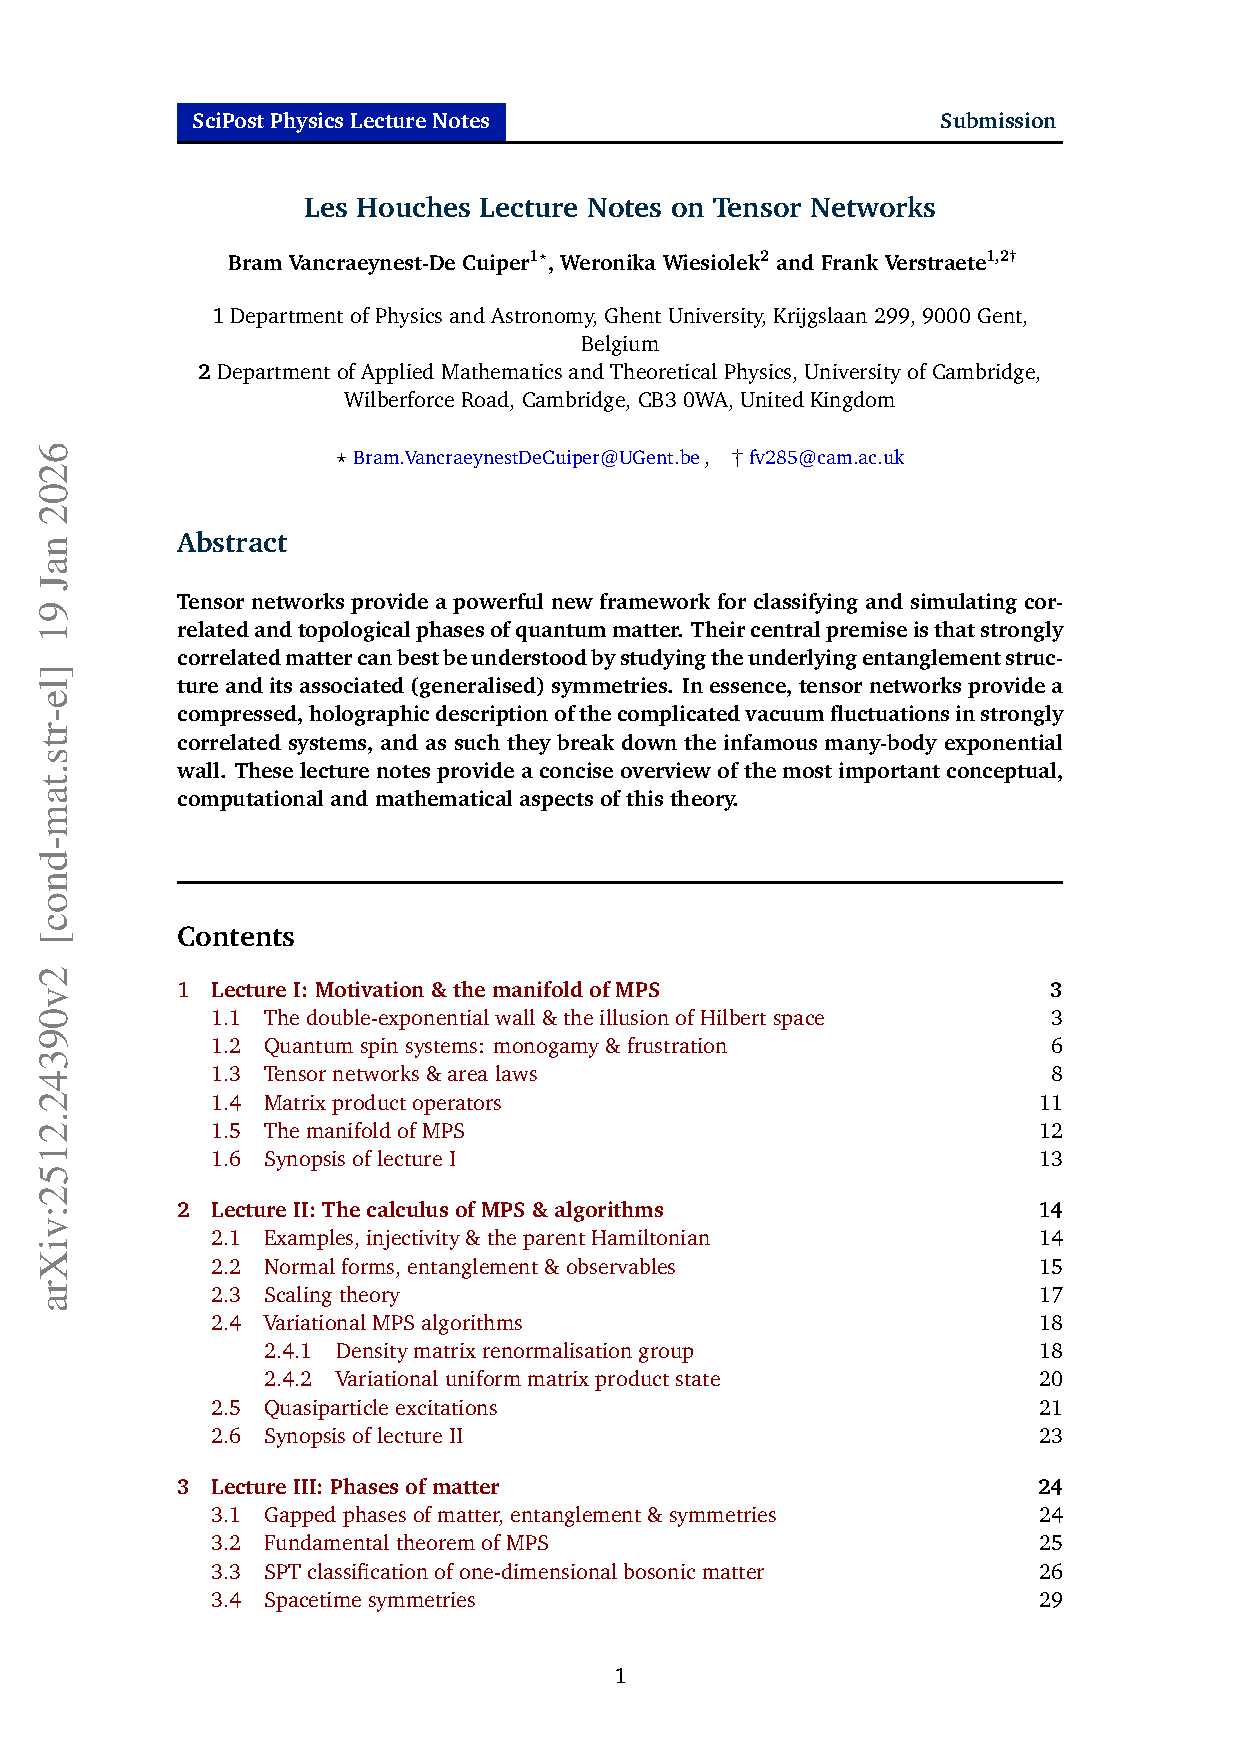
\includepdf[pages=1-4, trim=1.5cm 1.5cm 1.5cm 1.5cm, offset=-4mm 0mm, clip=true, frame=false, noautoscale=true, width=1.04\headwidth, pagecommand={}]{papers/lecture_notes}
%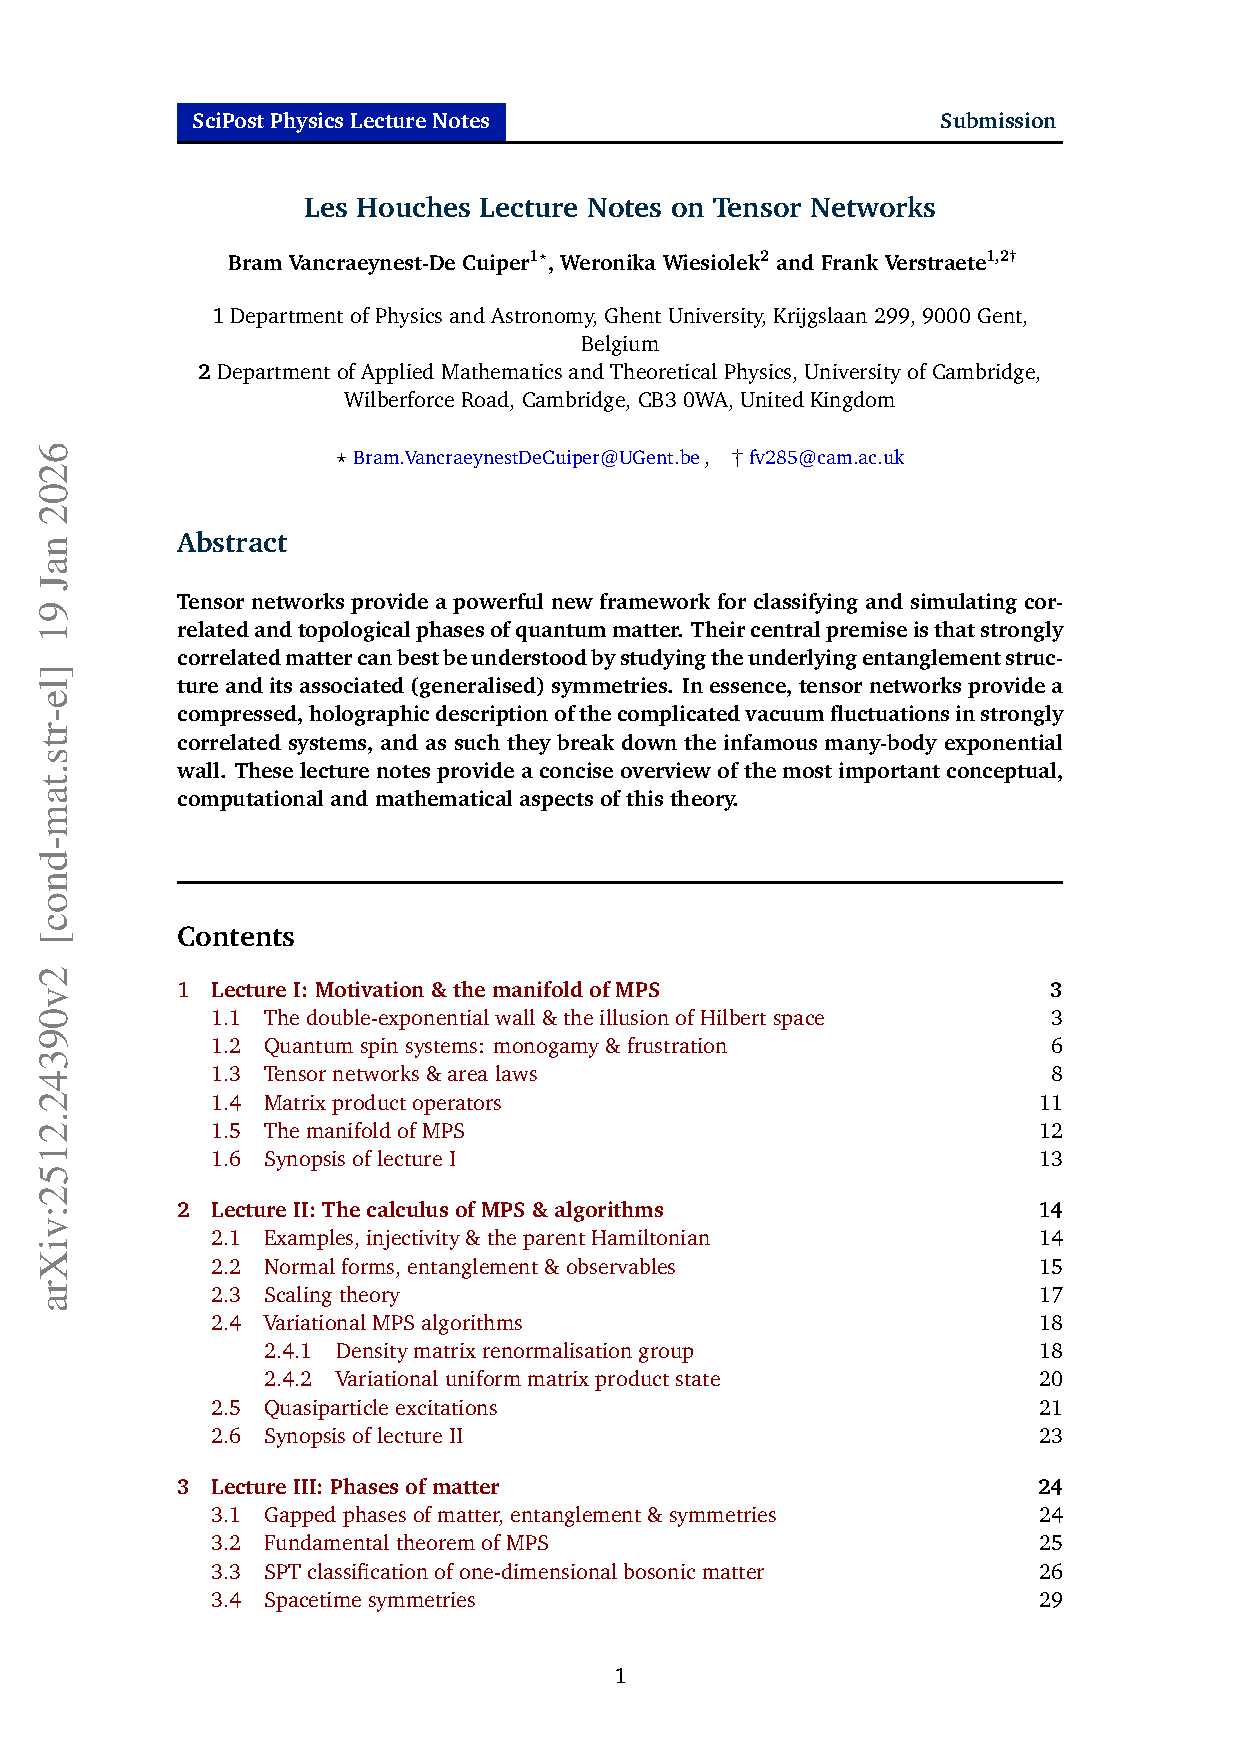
\includepdf[pages=-, trim=1.3cm 1.8cm 1.3cm 0cm, offset=-4mm 7mm, clip=true, frame=false, noautoscale=true, width=1.08\headwidth, pagecommand={}]{papers/lecture_notes}
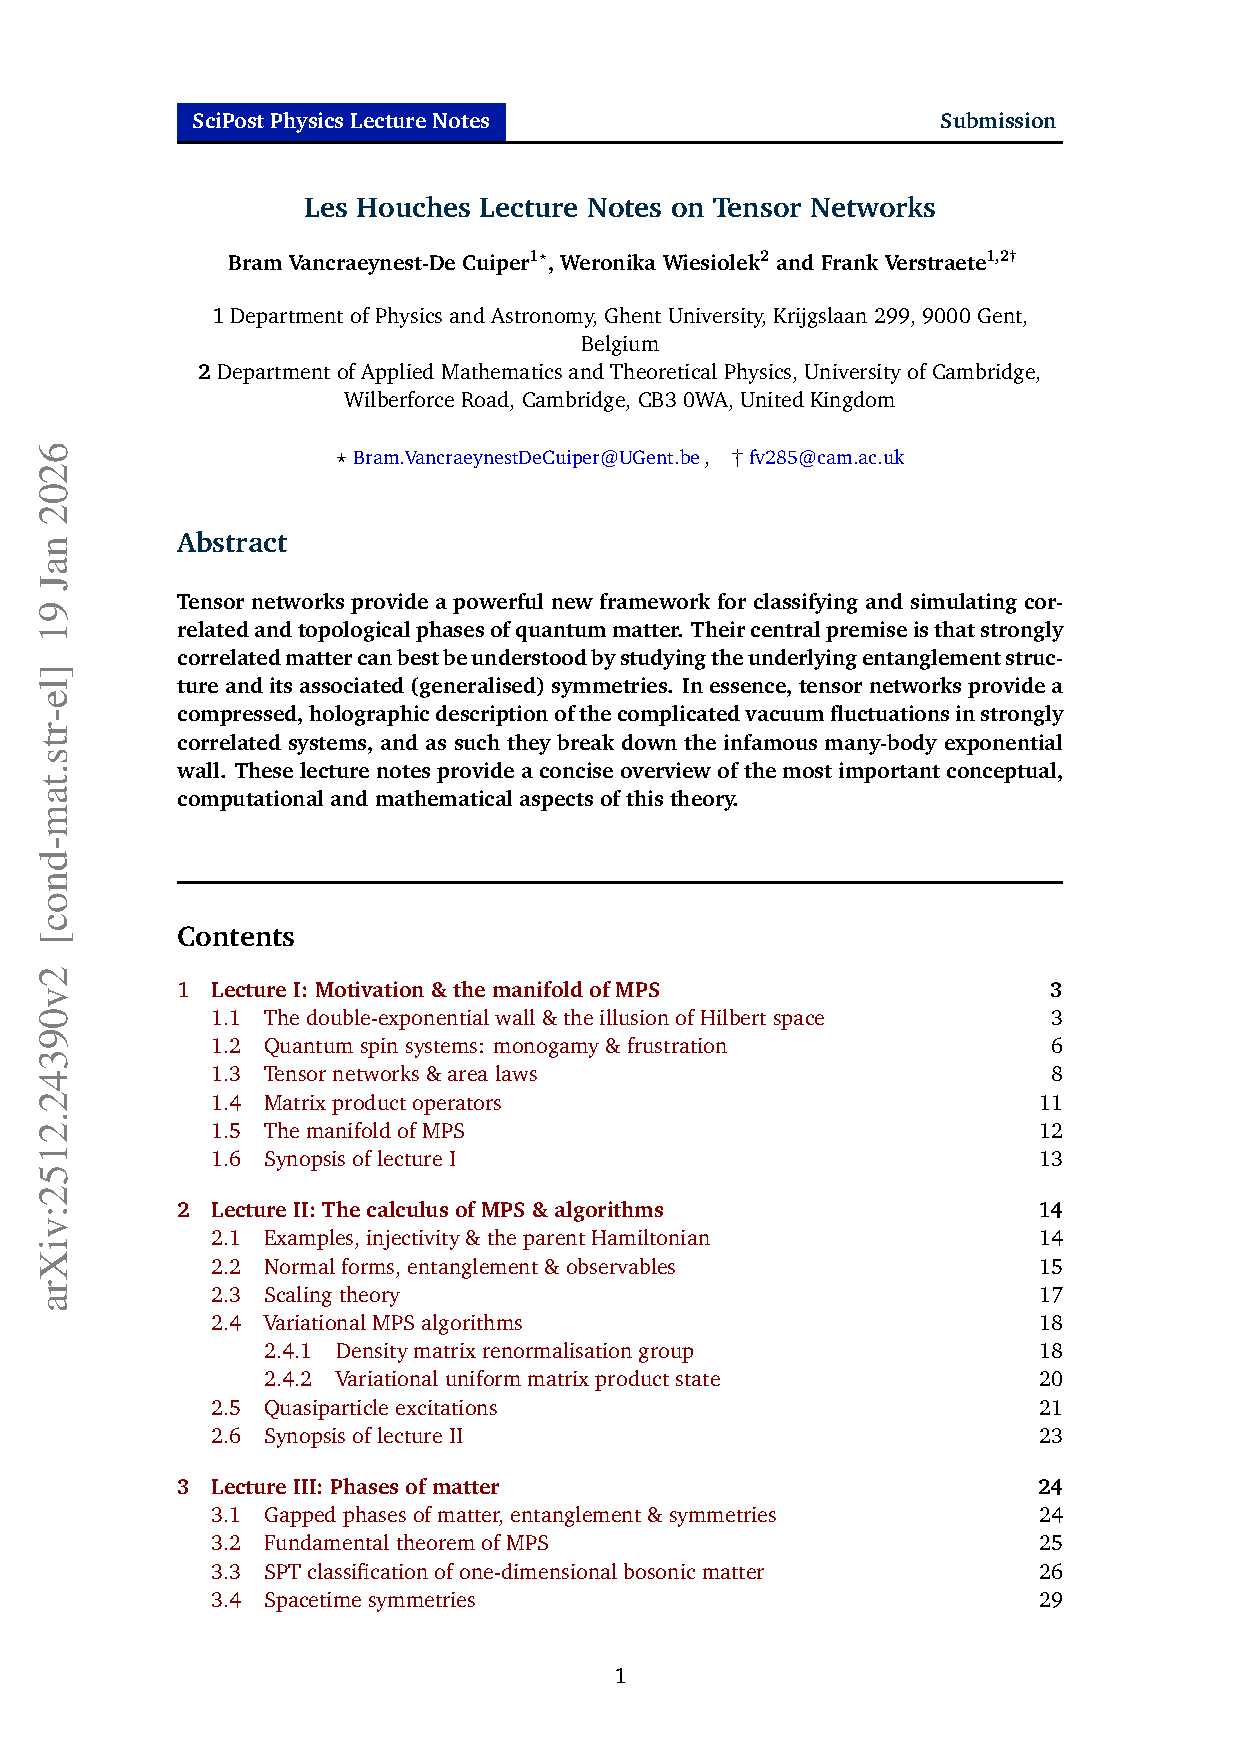
\includepdf[pages=-,
trim=25mm 20.54mm 25mm 18mm, clip=true,
noautoscale=true, height=\textheight,
offset=-0.65mm 4mm,
pagecommand={\thispagestyle{publication}}]{papers/lecture_notes}
\chapter{One-dimensional symmetric phases protected by frieze symmetries}\label{app:frieze}
\section{Synopsis}
In \cref{sec:1Dphases} we reviewed the classification of one-dimensional SPT phases protected by \emph{internal} symmetries acting in an on-site manner. The present project extends this classification to include quasi-one-dimensional \emph{spatial symmetries}. These are encoded in the so-called frieze groups, of which there are seven. We closely follow an approach analogous to that of \cref{sec:1Dphases} and study the action of the symmetry on an injective MPS. We find that these SPT phases are classified by the second cohomology group of the protecting symmetry group over $\rU(1)$, with the additional feature that \emph{orientation-reversing} group elements --- encoding spatial reflection, for instance --- act on $\rU(1)$ via complex conjugation. Additionally, we provide MPS normal forms for each of these phases and explicit renormalisation group fixed-point MPS representations directly in terms of representative cocycles. We also review the SPT classification in the presence of time-reversal symmetry. Finally, we discuss an algorithm that computes cohomology groups of any order and corresponding representative cocycles, including in the presence of non-trivial group action.
%TODO check if newpage is appropriate here
\newpage
\section{Reference}
\textit{One-dimensional symmetric phases protected by frieze symmetries} \par\noindent
\textbf{B. Vancraeynest-De Cuiper}, J. C. Bridgeman, N. Dewolf, J. Haegeman, F. Verstraete \par\noindent
\href{https://doi.org/10.1103/PhysRevB.107.115123}{Physical Review B \textbf{107} (11), 115123 (2023)}, \href{https://doi.org/10.48550/arXiv.2202.12880}{arXiv:2202.12880}
\section{Contributions of the author}
The project underlying this paper grew out of the Master's thesis of Nicolas Dewolf. Therein the classification of SPT phases protected by frieze symmetries was initiated and the framework established. I verified and completed the classification of MPS symmetric under these symmetry groups and their cohomological classification. I have finalised the algorithm based on the Smith normal form for computing group cohomology and cocycles and, conjointly with my supervisors, derived the representative fixed-point matrix product states. The manuscript was mostly written by me.

%\section{One-dimensional symmetric phases protected by frieze symmetries}
%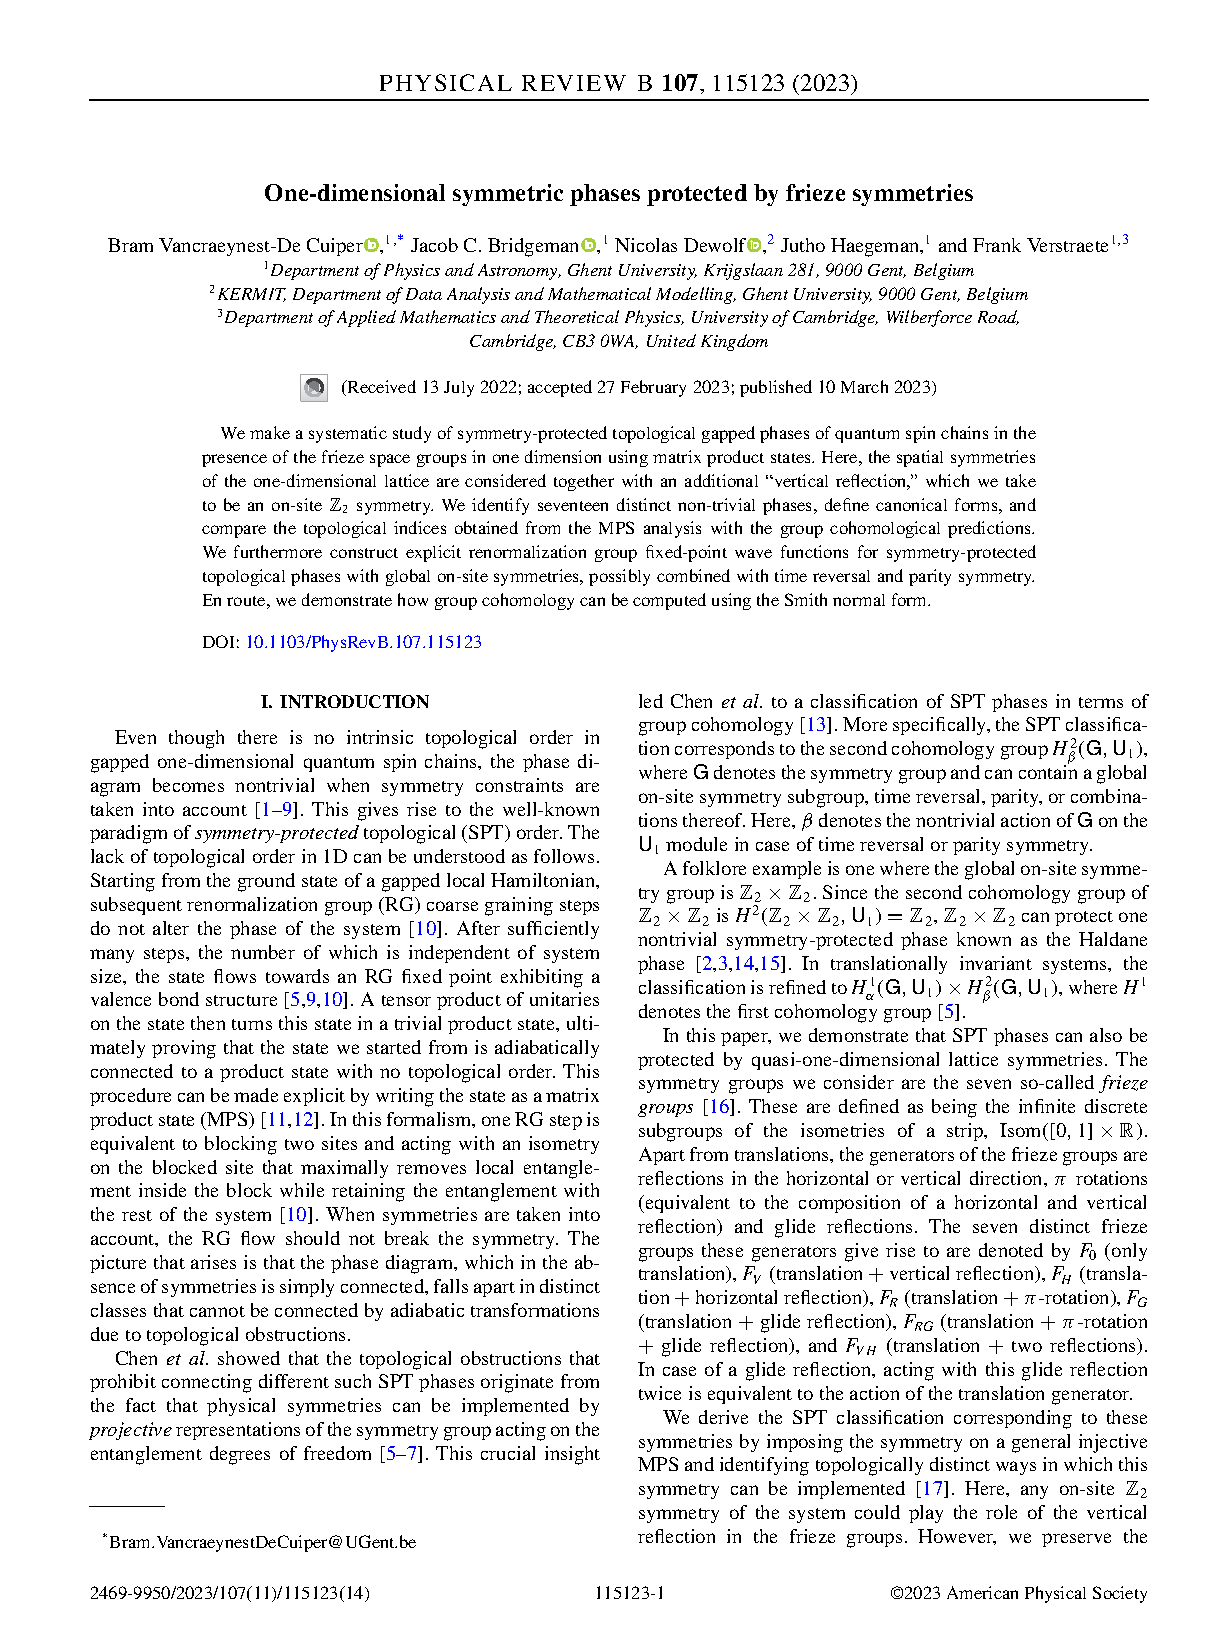
\includepdf[pages=-, trim=0 1.2cm 0 1.2cm, clip=true, frame=false, noautoscale=true, width=1.14\headwidth, offset=-4mm 6mm, , pagecommand={}]{papers/frieze}
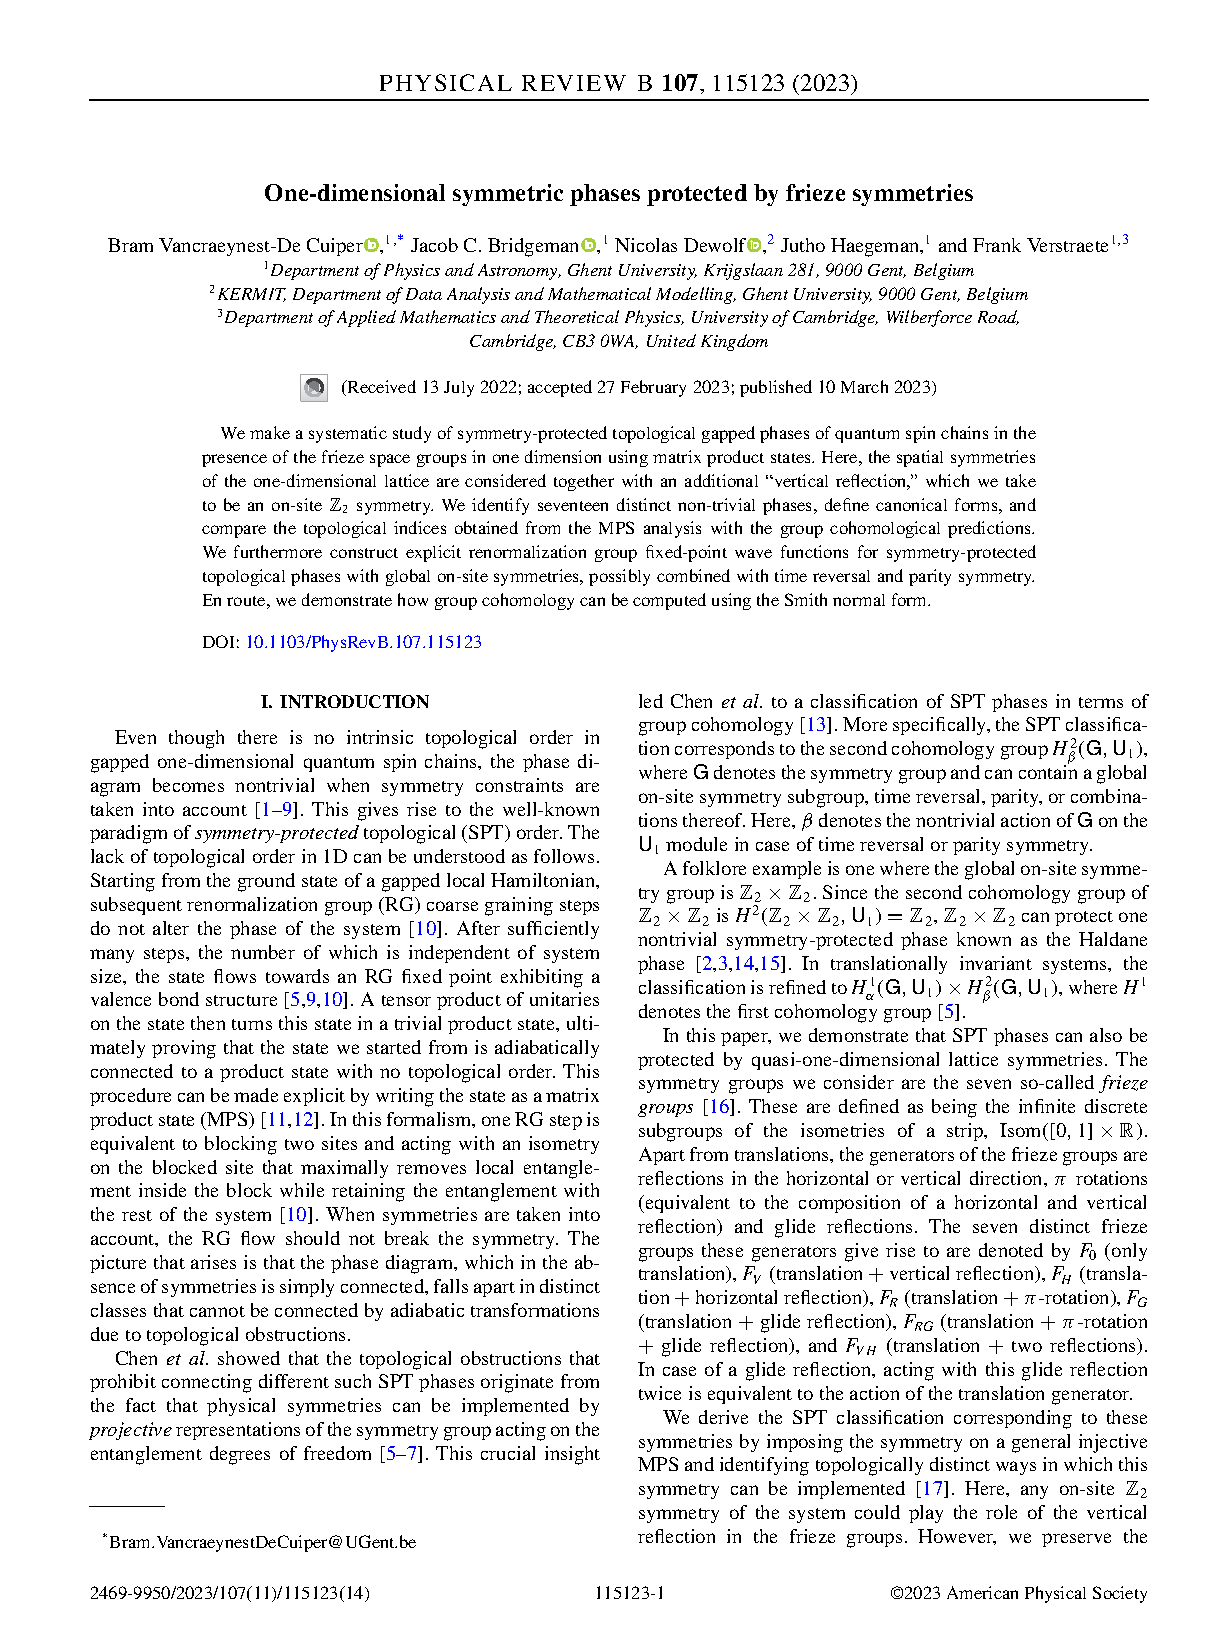
\includepdf[pages=-,
trim=12mm 12.7mm 12mm 9.2mm, clip=true,
noautoscale=true, width=\textwidth,
offset=-0.65mm 5mm,
pagecommand={\thispagestyle{publication}}]{papers/frieze}
\chapter{Mapping between Morita equivalent string-net states with a constant depth quantum circuit}\label{app:SN}
\section{Synopsis}
As argued in \cref{eq:SymGappedPhases}, two models belong to the same gapped quantum phase of matter if they are related by an interpolating quantum circuit of sublinear depth. In this project, we explicitly construct such a constant-depth circuit for string-net models whose input UFCs $\mc D_1$ and $\mc D_2$ are \emph{Morita equivalent}. The circuit is built explicitly from the $F$-symbols encoded in an invertible $(\mc D_1,\mc D_2)$-bimodule category.

Concretely, we first review in detail the framework of \emph{extended string-net models}, mentioned above in \cref{sec:LoopsExcited}. These extended string-nets provide a framework in which all anyonic excitations encoded in $\mc Z(\mc D)$, including those violating vertex Hamiltonian terms, can be treated in a unified manner. We then use the aforementioned associator data encoded in an invertible $(\mc D_1,\mc D_2)$-bimodule category to define the quantum circuit and compute its action on both ground and excited states. When restricted to the ground state sector, the circuit reduces precisely to the generalised ground-state projector introduced in \cref{sec:SNPEPS}. Its action on excited states on the other hand requires the introduction of ancillary degrees of freedom that account for mismatches in the dimensions of the central idempotents describing the anyons in the two theories. In that case, the circuit acts on individual plaquettes via \emph{bimodule tubes}, akin to those introduced in \cref{sec:SymTwist}.

As an illustrative example, we show that, when applied to the \emph{toric code}, our construction reproduces the familiar \emph{electric–magnetic duality}. More generally, for \emph{quantum double models} based on possibly non-abelian input groups, it recovers a quantum circuit previously introduced in refs.~\cite{Buerschaper2009b,Kadar2009}.
\section{Reference}
\textit{Mapping between Morita equivalent string-net states with a constant depth quantum circuit} \par\noindent
L. Lootens, \textbf{B. Vancraeynest-De Cuiper}, N. Schuch, F. Verstraete \par\noindent
\href{https://doi.org/10.1103/PhysRevB.105.085130}{Physical Review B \textbf{105} (8), 085130 (2022)}, \href{https://doi.org/10.48550/arXiv.2112.12757}{arXiv:2112.12757}
\section{Contributions of the author}
The central idea underlying this project, together with its overall technical framework, was developed by Laurens Lootens in collaboration with Norbert Schuch and Frank Verstraete. My primary contribution was the explicit derivation of the quantum circuit in terms of the bimodule data, which is the main result underlying this project. In addition, I contributed to the writing of the manuscript, including portions of the review of extended string-net models, the presentation of the quantum circuit, and the example section.
%\section{Mapping between Morita equivalent string-net states with a constant depth quantum circuit}
%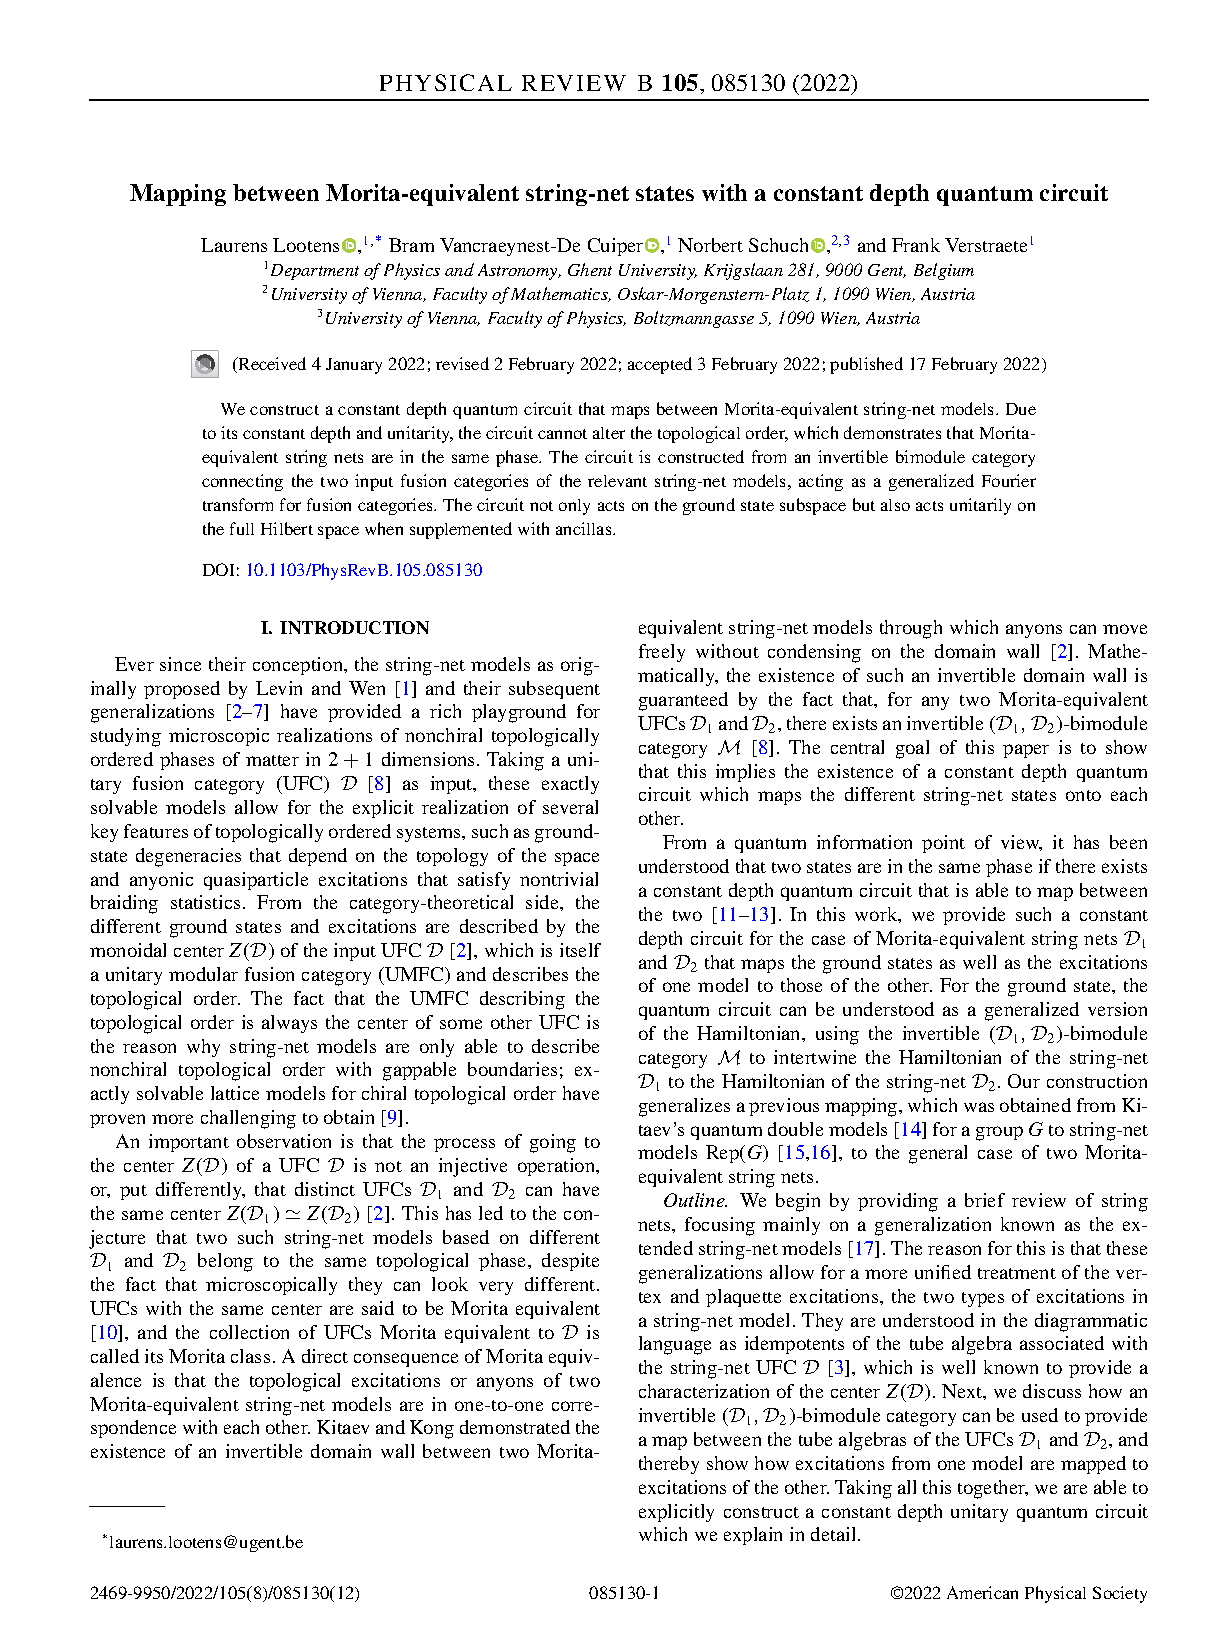
\includepdf[pages=-, trim=0 1.2cm 0 0, clip=true, frame=false, noautoscale=true, width=1.14\headwidth, offset=-4mm 6mm, , pagecommand={}]{papers/string_net}
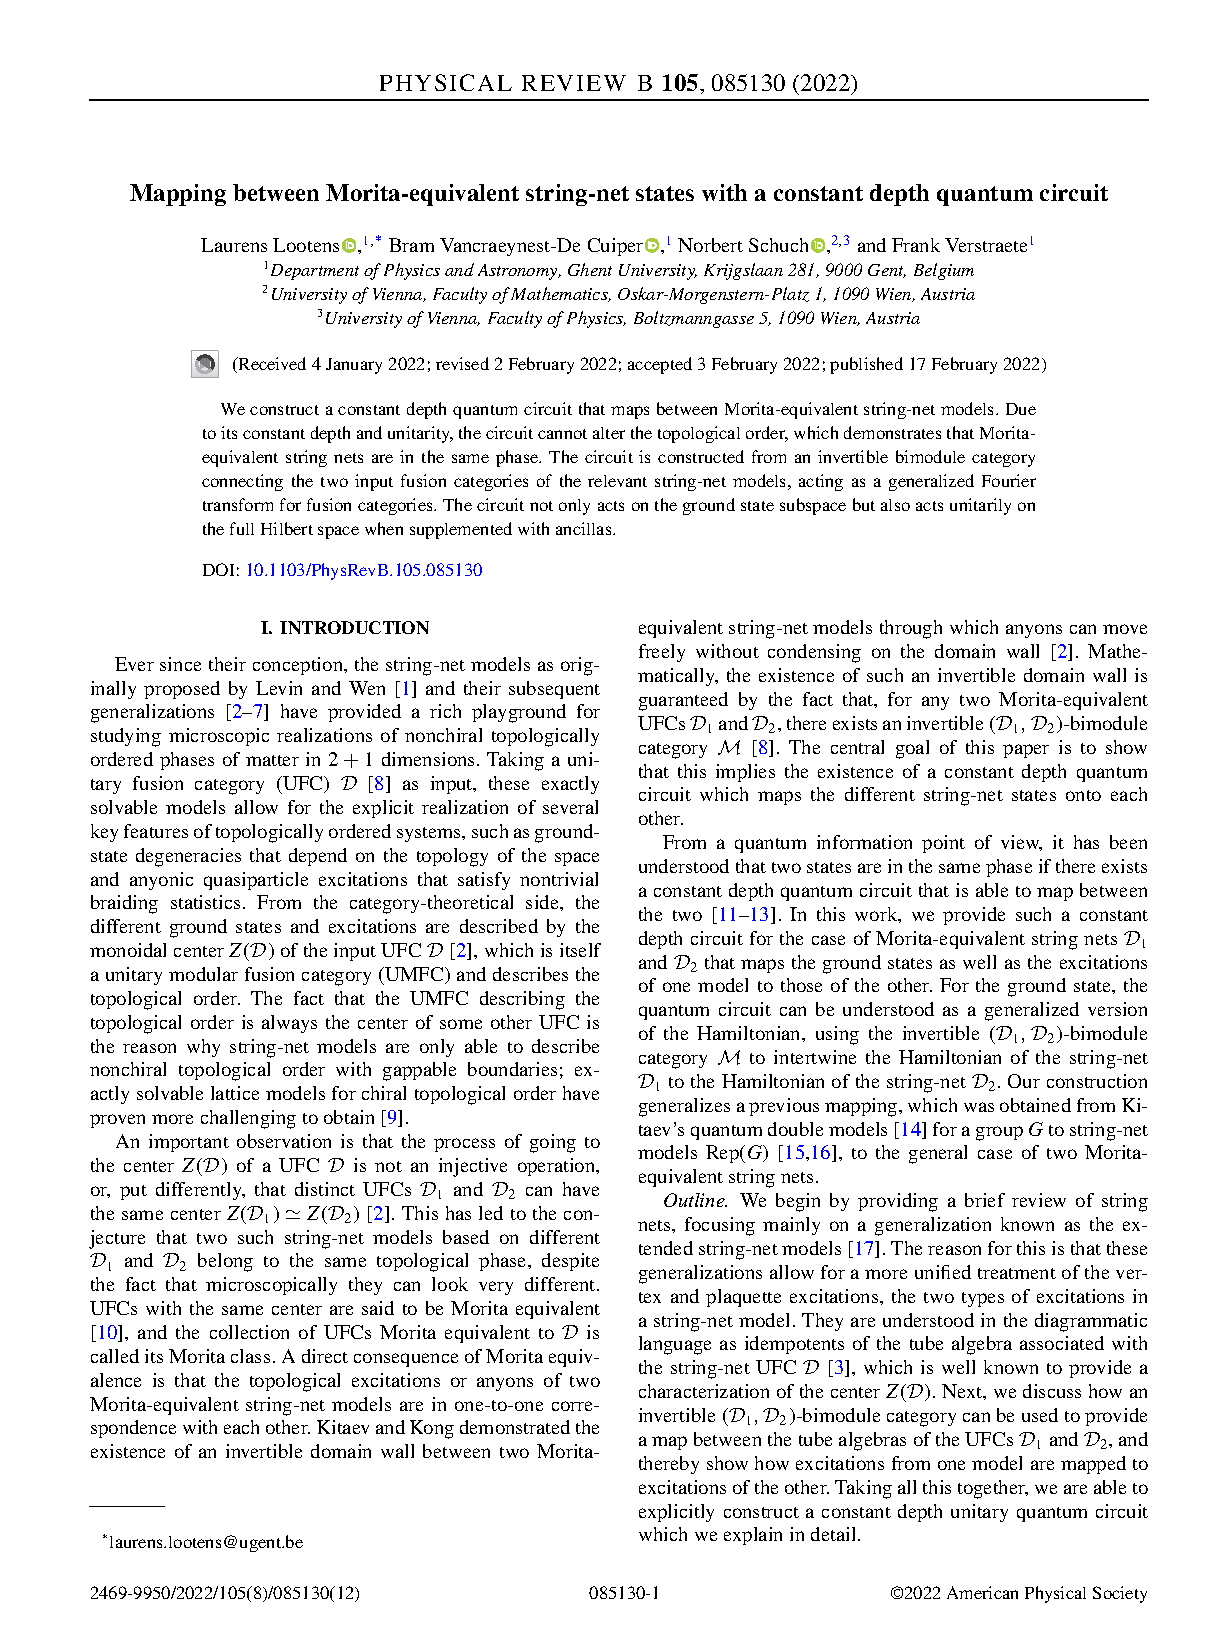
\includepdf[pages=-,
trim=12mm 12.7mm 12mm 9.2mm, clip=true,
noautoscale=true, width=\textwidth,
offset=-0.65mm 5mm,
pagecommand={\thispagestyle{publication}}]{papers/string_net}
\chapter{From gauging to duality in one-dimensional	quantum lattice models}\label{app:gauging}

\section{Synopsis}
It is well known that gaugings of $\mc C$-symmetric two-dimensional quantum field theories are encoded by (Frobenius) \emph{algebra objects} $A$ in $\mc C$~\cite{Fuchs2002,Bhardwaj2017}. These algebra objects specify both a gaugeable collection of topological lines and a generalised notion of \emph{discrete torsion} through their multiplication map. In this project, we extend the gauging map of Haegeman et al. ~\cite{Haegeman2014a}, initially defined for non-anomalous group symmetries, to incorporate genuine categorical symmetries and show that a choice of algebra object precisely captures the data required for this generalisation. Our construction recovers the results of ref.~\cite{Haegeman2014a} for the symmetry category $\Vect_G$, and agrees with a parallel work that discusses gauging algebra objects on the lattice, where they overlap~\cite{Seifnashri2025}. We further demonstrate that, up to constant-depth \emph{disentangling} unitary quantum circuits, the resulting gauging maps are equivalent to the duality intertwiners introduced in refs.~\cite{Lootens2021b,Lootens2022} and discussed in \cref{sec:dualities}. In addition, we consider the inclusion of symmetry-twisted boundary conditions, present several non-trivial examples, and prove the existence of a symmetric and injective matrix product state when $\mc C$ describes an anomaly-free symmetry and is thus fully gaugeable.
\newpage
\section{Reference}
\textit{From gauging to duality in one-dimensional	quantum lattice models} \par\noindent
\textbf{B. Vancraeynest-De Cuiper}, J. Garre-Rubio, F. Verstraete, K. Vervoort, D. J. Williamson, L. Lootens \par\noindent
\href{https:/doi.org/10.21468/SciPostPhys.20.4.113}{SciPost Phys. \textbf{20}, 113 (2026)}, \href{https://doi.org/10.48550/arXiv.2509.22051}{arXiv:2509.22051}
\section{Contributions of the author}
This project was conceived by José Garre-Rubio and Laurens Lootens. I derived the gauging map and the disentangling unitary transformation, in collaboration with Laurens Lootens. The gauging map in the presence of symmetry twists, as well as the examples are due to me. I wrote the manuscript, with the exception of section 5 which is written by Laurens Lootens.
%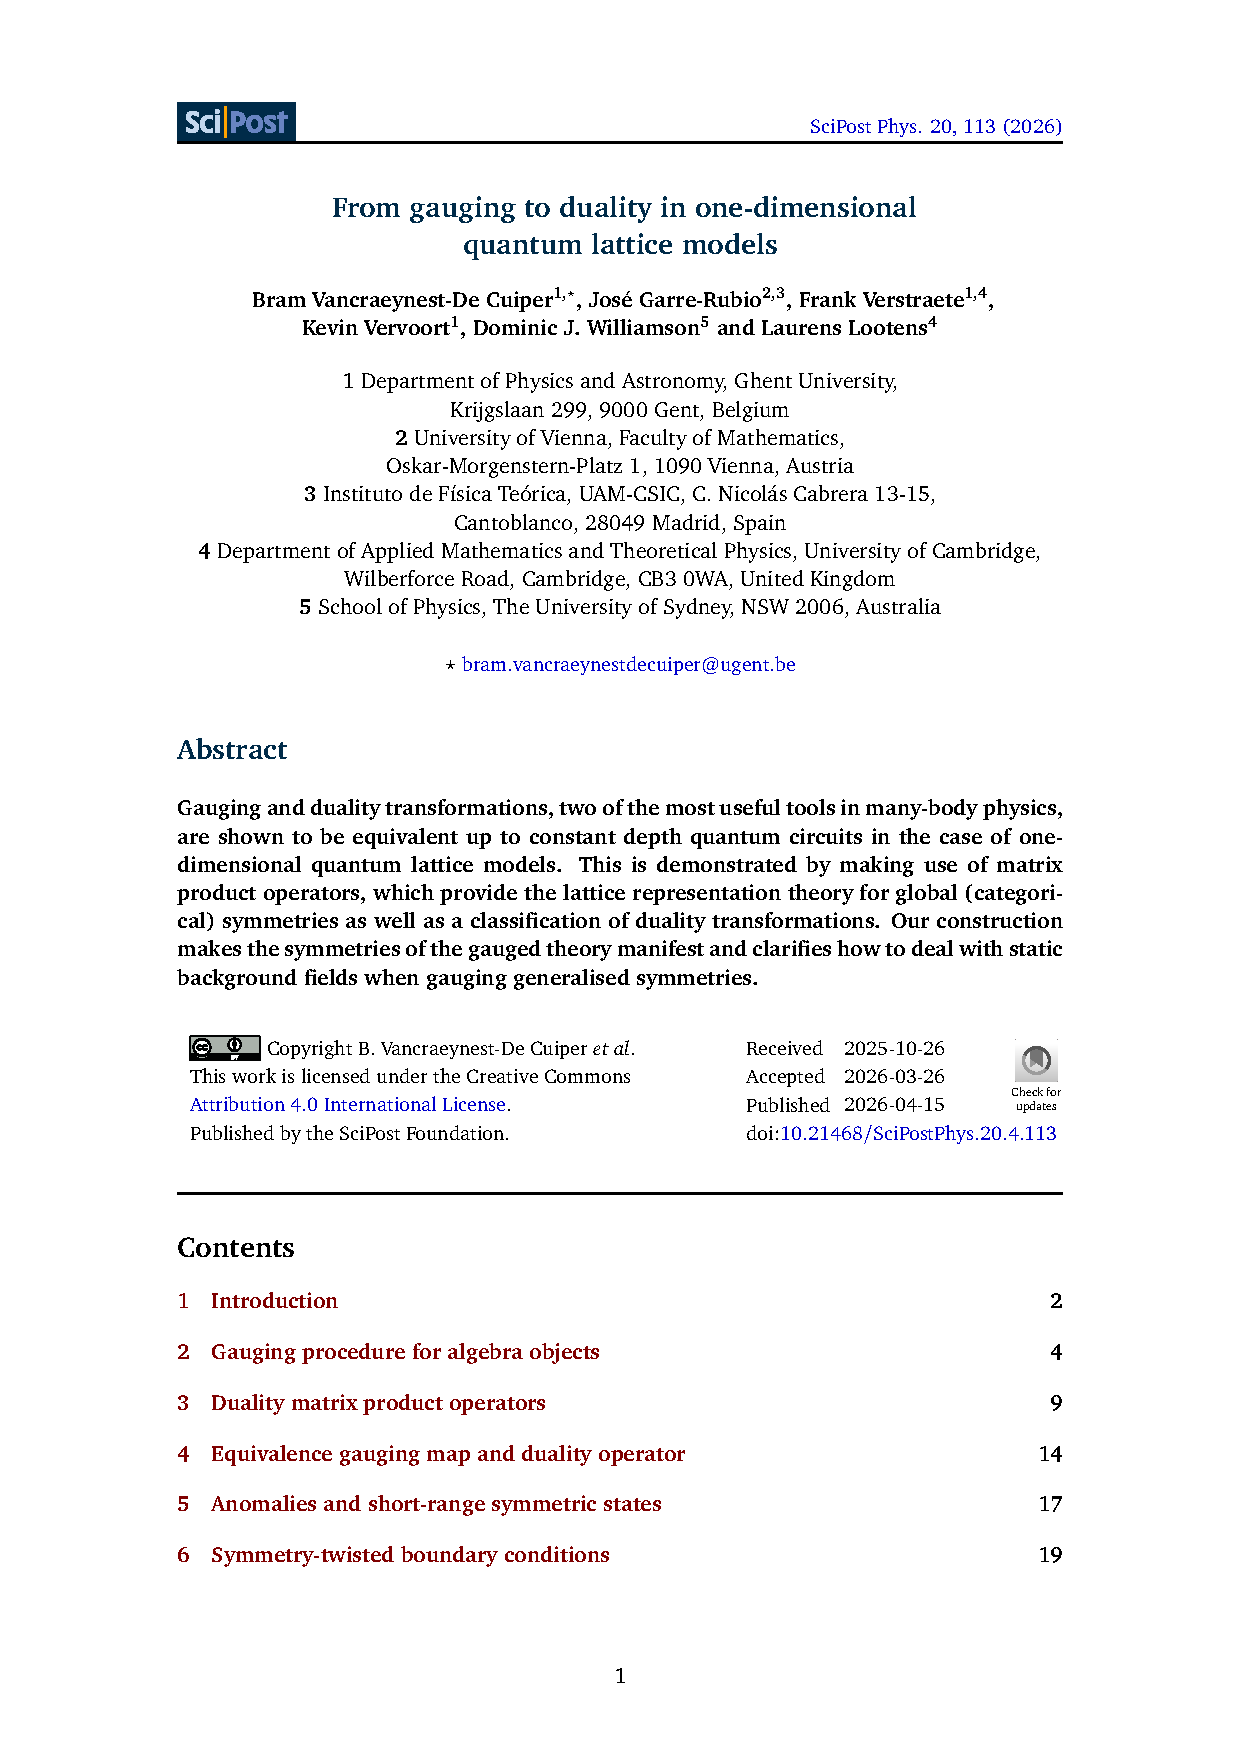
\includepdf[pages=-, trim=1.3cm 1.8cm 1.3cm 0cm, offset=-4mm 7mm, clip=true, frame=false, noautoscale=true, width=1.08\headwidth, pagecommand={}]{papers/gauging}
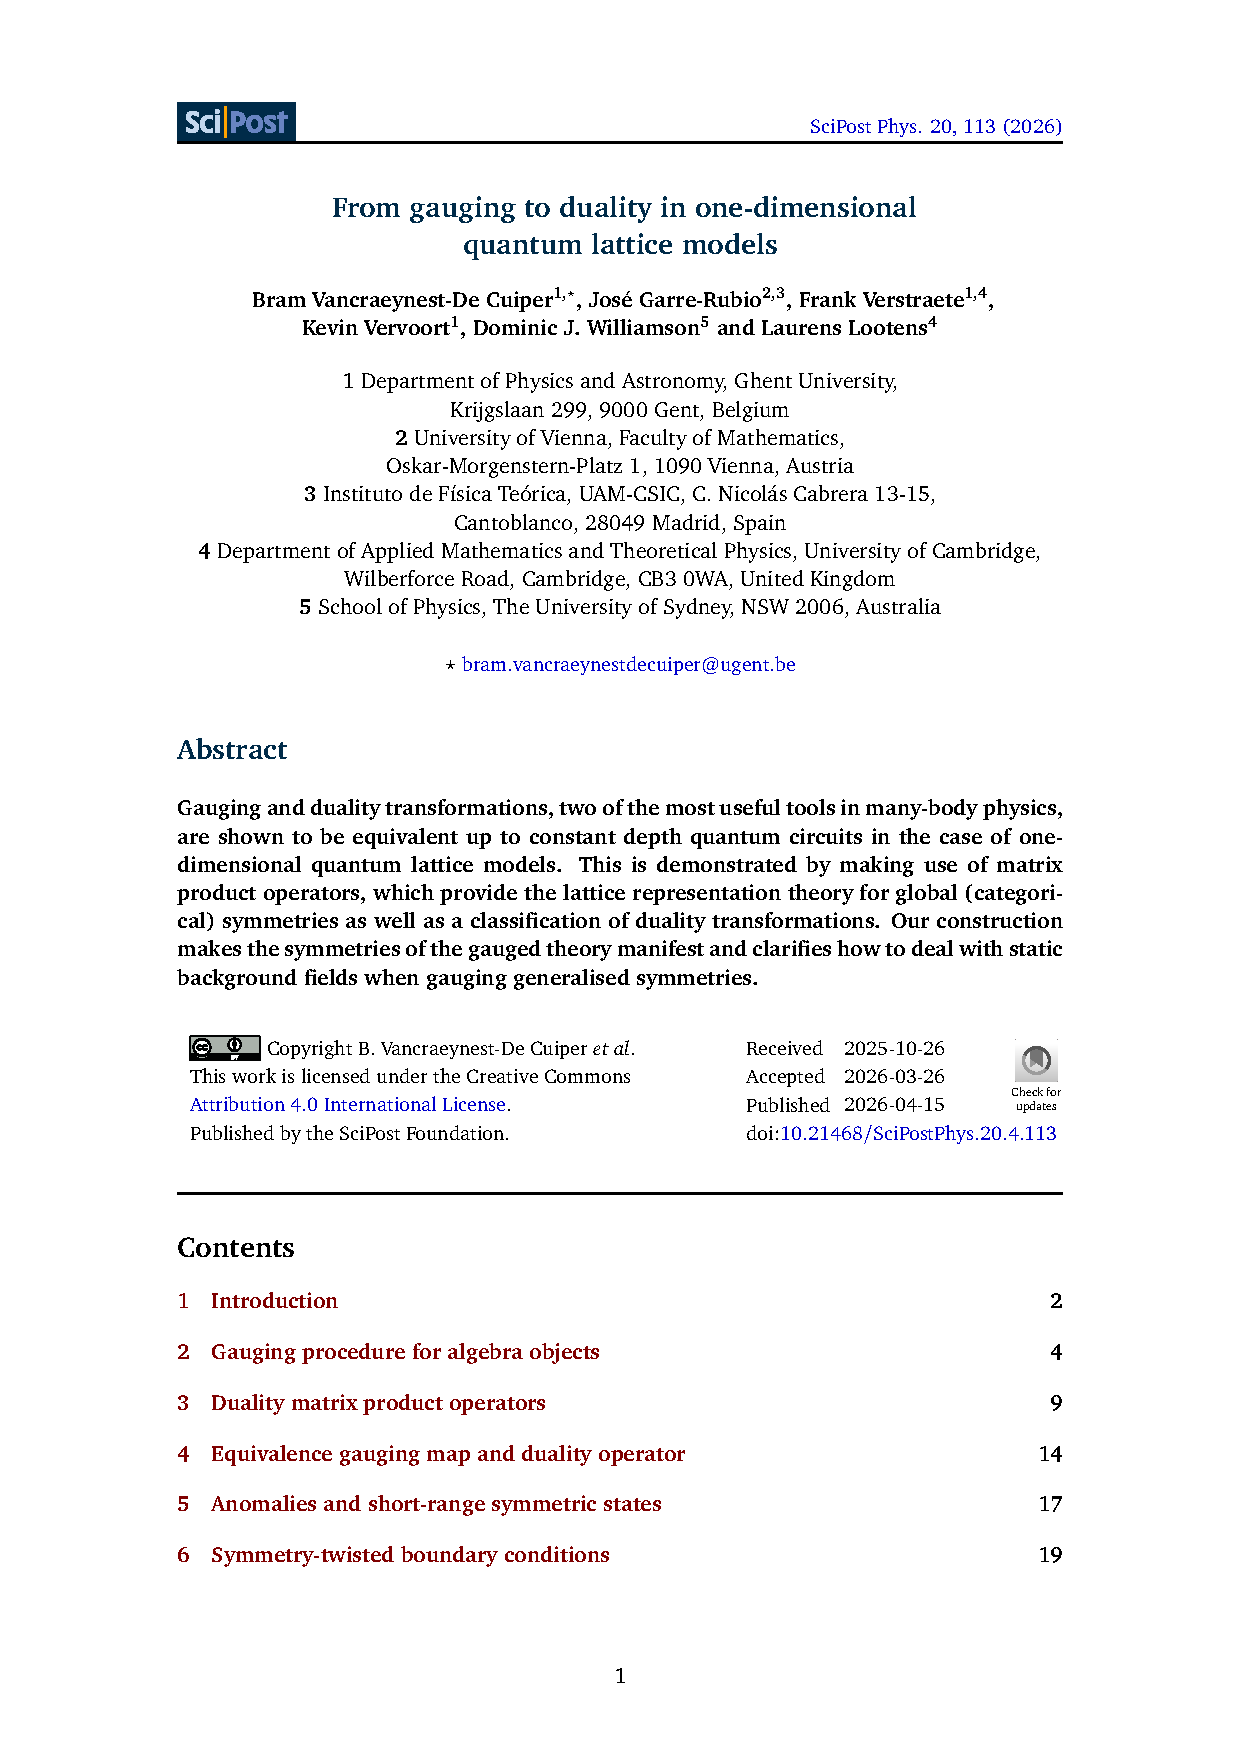
\includepdf[pages=-,
trim=25mm 20.54mm 25mm 17mm, clip=true,
noautoscale=true, height=\textheight,
offset=-0.65mm 4mm,
pagecommand={\thispagestyle{publication}}]{papers/gauging}
\chapter{Systematic construction of stabilizer codes via gauging abelian boundary symmetries}\label{app:codes}
\section{Synopsis}
In this project, we generalise a construction of the second author, published in ref.~\cite{GarreRubio2024}, to arbitrary spatial dimensions. Starting from a generic $d$-dimensional quantum state with an \emph{abelian} symmetry, we iteratively gauge the symmetry and its dual to obtain a state in one dimension higher. The admissible initial symmetries include global 0-form, higher-form, \emph{subsystem} and \emph{fractal symmetry}.

The resulting $(d+1)$-dimensional state naturally inherits this original symmetry at its boundary and can be shown to be the ground state of a local commuting projector Hamiltonian. The construction relies on an extension, developed in this work, of Williamson’s gauging procedure of \emph{submanifold symmetries}~\cite{Williamson2016b}. We formulate the framework in terms of tensor networks, where gauging maps are implemented as tensor network operators akin to those of ref.~\cite{Haegeman2014a}. The composition of these then provides a tensor network representation of the one-higher-dimensional state.

We illustrate the approach through several examples, including three-dimensional \emph{Clifford-deformed surface codes} and \emph{type-I fracton phases} obtained by gauging linear subsystem and \emph{Sierpinski} fractal symmetries.
\section{Reference}
\textit{Systematic construction of stabilizer codes via gauging abelian boundary symmetries} \par\noindent
\textbf{B. Vancraeynest-De Cuiper}, J. Garre-Rubio \par\noindent
\href{https:/doi.org/10.22331/q-2025-09-08-1852}{Quantum \textbf{9}, 1852 (2025)}, \href{https://doi.org/10.48550/arXiv.2410.09044}{arXiv:2410.09044}
\section{Contributions of the author}
%The current project is a generalisation of the construction developed in ref.~\cite{GarreRubio2024} by Jos\'e Garre-Rubio to arbitrary dimensions and general abelian symmetries. 

The main technical result underlying this project consists of a generalisation of the gauging procedure of Williamson, which in its original form was formulated for the symmetry group $\mbb Z_2$, to arbitrary abelian groups~\cite{Williamson2016b}. I derived this generalised gauging procedure and its associated dual symmetries conjointly with my co-author. The iterative gauging procedure is then obtained from this gauging procedure, the tensor network representation of which was constructed by me. I derived the introductory example of section 1, as well as the boundary conditions of the models appearing in sections 3 and 4. I wrote the majority of the manuscript.
%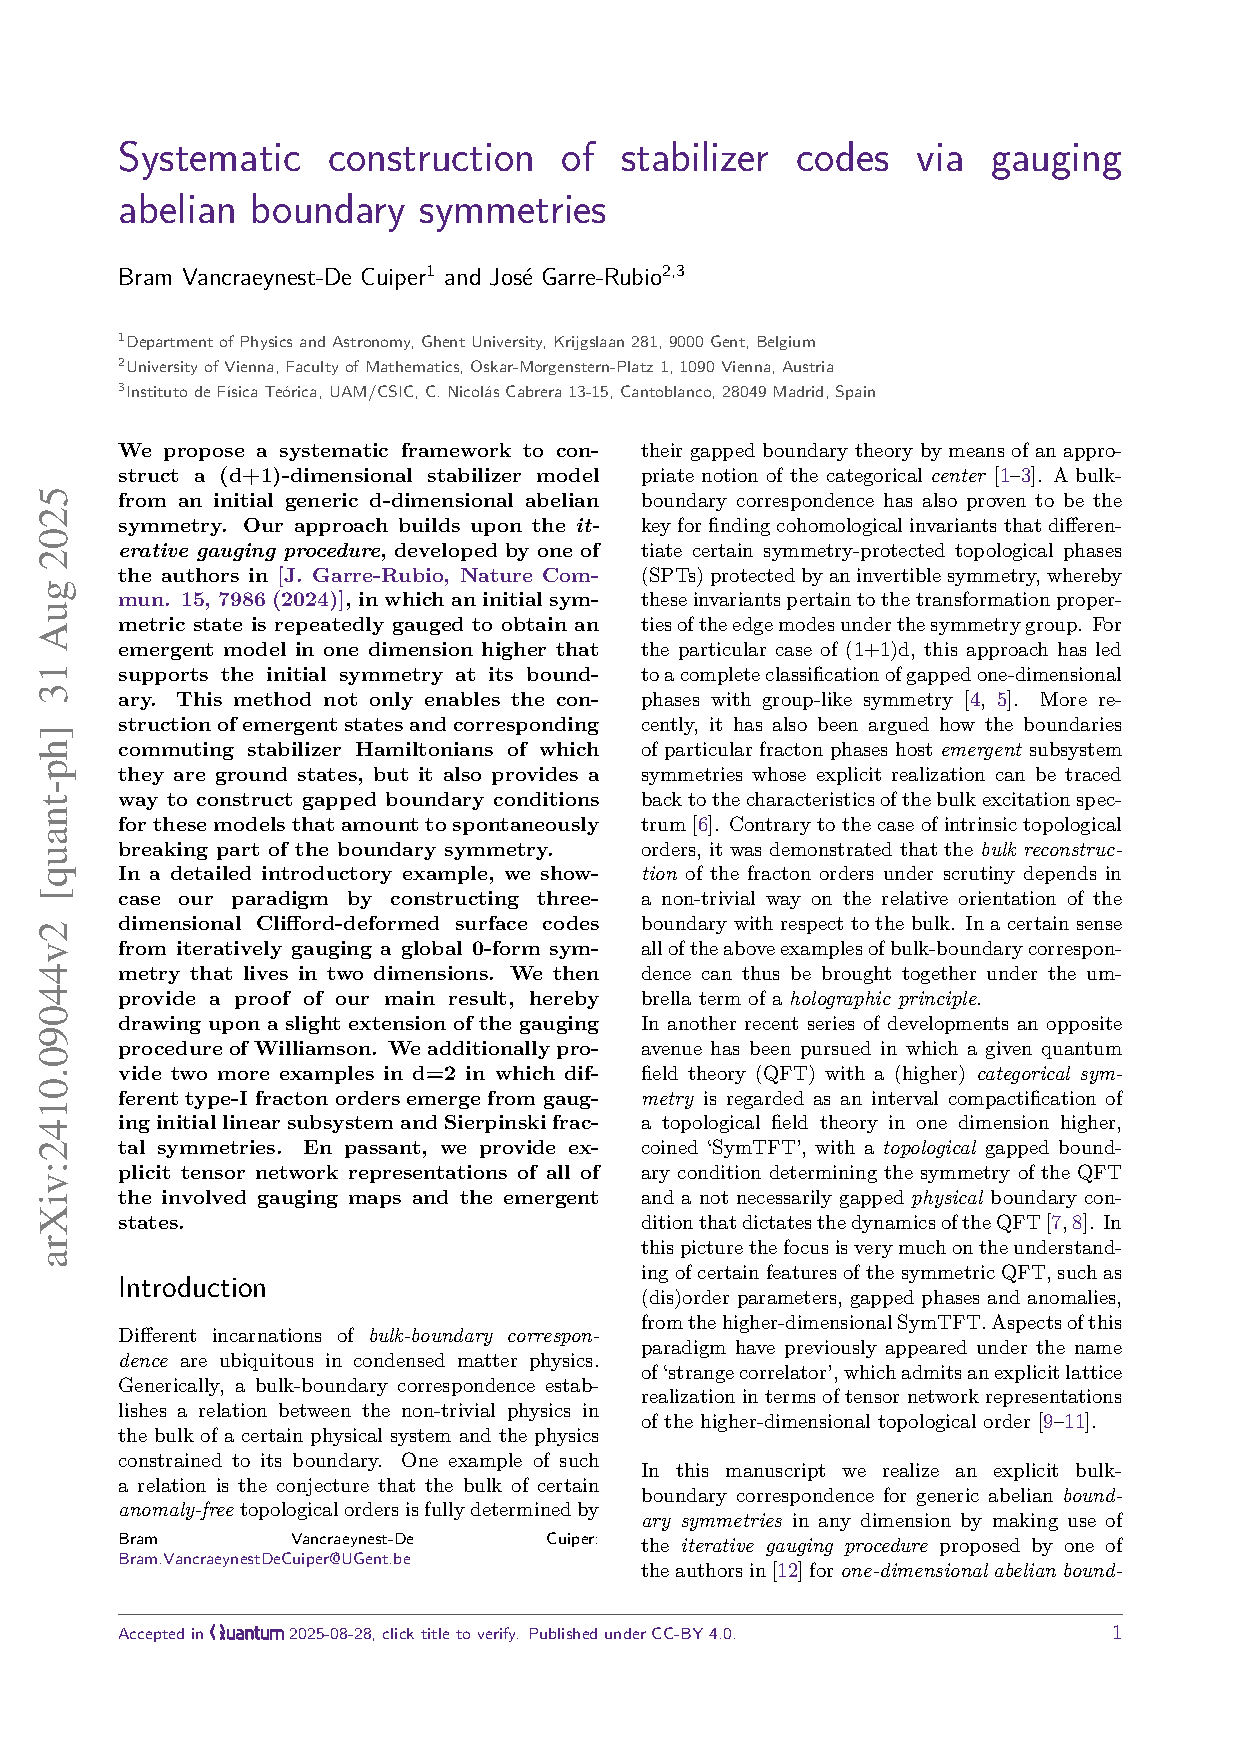
\includepdf[pages=-, trim=1.4cm 2.5cm 1.3cm 1cm, offset=-4mm 7mm, clip=true, frame=false, noautoscale=true, width=1.07\headwidth, pagecommand={}]{papers/stabilizers}
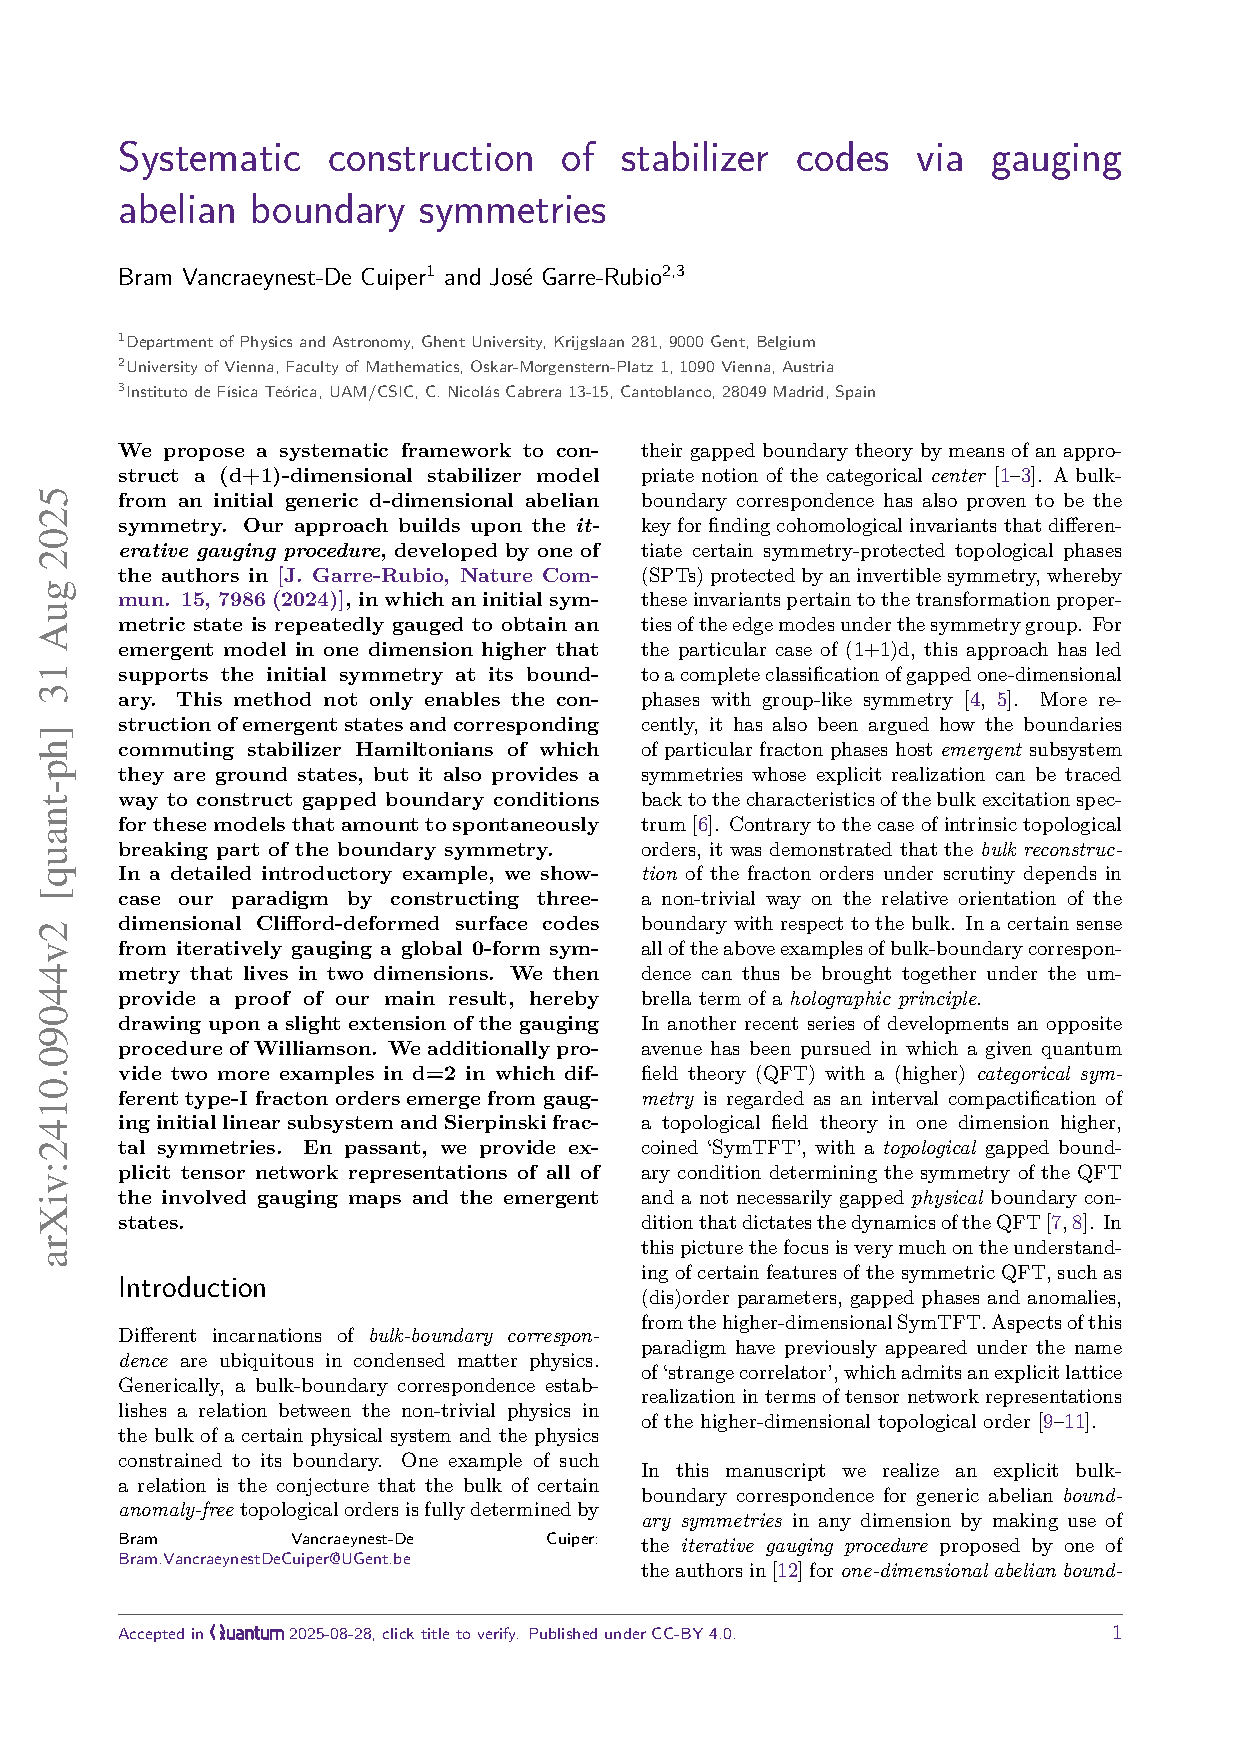
\includepdf[pages=-,
trim=17mm 27mm 17mm 17mm, clip=true,
noautoscale=true, width=\textwidth,
offset=-0.65mm 0mm,
pagecommand={\thispagestyle{publication}}]{papers/stabilizers}
\chapter{Twisted gauging and topological sectors in (2+1)d abelian lattice gauge theories}\label{app:TwistedGauging}
\section{Synopsis}
An open problem in the study of three-dimensional quantum field theories is the construction of genuinely \emph{self-dual} models --- that is, models that are mapped to themselves under some duality transformation. Necessarily, such a self-duality should preserve the symmetry structure of either model. A central observation of ref.~\cite{Decoppet2023} is that a specific class of gauging and twisted gauging transformations appears to be the only mechanism capable of producing such self-dual theories in this dimension.

The duality transformations we study in this project intertwine (2+1)-dimensional \emph{twisted Abelian lattice gauge theories} whose symmetry structure is encoded by the fusion 2-category $\TRep(G)$, which simultaneously captures Wilson line operators as 1-form symmetry operators, their condensation defects as 0-form symmetry operators, as well as topological interfaces between those membrane operators. The duality transformation amounts to the change in module 2-category $\TVect\mapsto\TVect^\alpha$ over the input $\TVect_G$, with $[\alpha]\in H^3(G,\rU(1))$ encoding the aforementioned twist or discrete torsion. Physically, this map amounts to the gauging of the 1-form symmetry of the theory, followed by a twisted gauging of the resulting 0-form $\TVect_G$ symmetry. We provide lattice representations of these symmetry operators and duality intertwiners in the form of topological matrix product operators and projected entangled-pair operators. We characterise the 1-form symmetry-twisted boundary conditions and charge sectors, and construct the unitary duality transformations that relate the dual theories to one another.

We first illustrate the mechanism in one spatial dimension, where the construction for the case of $G=\ZtZt$, with the non-trivial twist $[\psi]$ valued in $H^2(\ZtZt,\rU(1))\simeq\mbb Z_2$, reduces to the \emph{Kennedy-Tasaki duality}~\cite{Kennedy1992} and which serves as an introduction to the higher-dimensional case. In two spatial dimensions, we work out an explicit realisation of the duality between the \emph{toric code} and the \emph{double semion} model corresponding to the string-net model with $\Vect_{\mbb Z_2}$, respectively $\Vect_{\mbb Z_2}^\alpha$, as input, $[\alpha]$ being the non-trivial class in $H^3(\mbb Z_2,\rU(1))\simeq\mbb Z_2$~\cite{Kitaev1997,Levin2004,Levin2012}. Finally, we show that the sum of these two models admits an interpretation as a \emph{higher gauge theory}, in which the duality transformation is promoted to a genuine internal symmetry.
\section{Reference}
\textit{Twisted gauging and topological sectors in (2+1)d abelian lattice gauge theories} \par\noindent
\textbf{B. Vancraeynest-De Cuiper}, C. Delcamp \par\noindent
\href{https:/doi.org/10.21468/SciPostPhys.19.2.054}{SciPost Phys. \textbf{19}, 054 (2025)}, \href{https://doi.org/10.48550/arXiv.2501.16301}{arXiv:2501.16301}
\section{Contributions of the author}
This project was mainly conceived by Clement Delcamp, who developed the overarching conceptual framework based on earlier work~\cite{Delcamp2021,Delcamp2023}. He wrote the majority of the manuscript. My contributions focused primarily on the derivations related to the one-dimensional dualities, including the mapping of topological sectors and order parameters. I additionally contributed to the two-dimensional case, in particular with regard to the symmetries and boundary conditions of the two-dimensional models. I also co-wrote sections of the paper.
%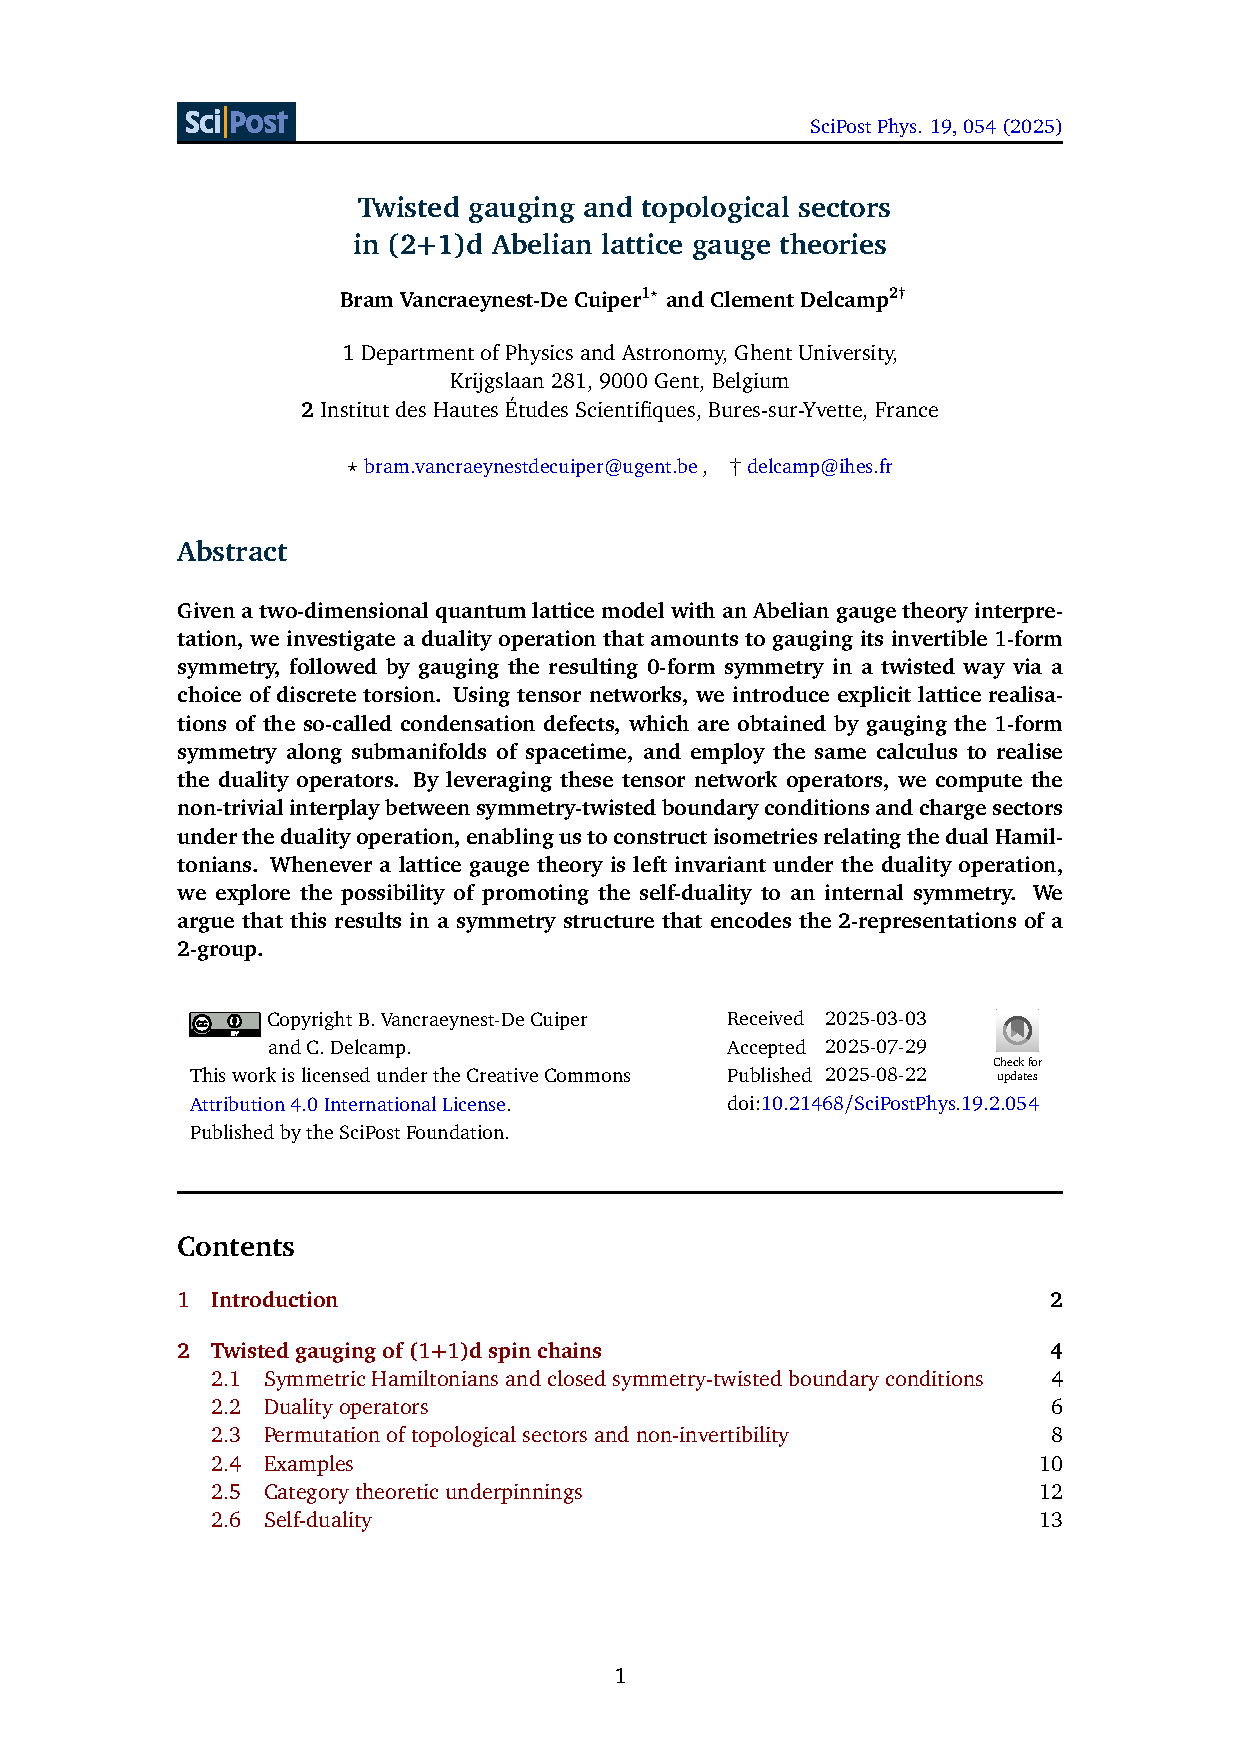
\includepdf[pages=-, trim=1.3cm 1.8cm 1.3cm 0cm, offset=-4mm 7mm, clip=true, frame=false, noautoscale=true, width=1.08\headwidth, pagecommand={}]{papers/twisted_gauging}
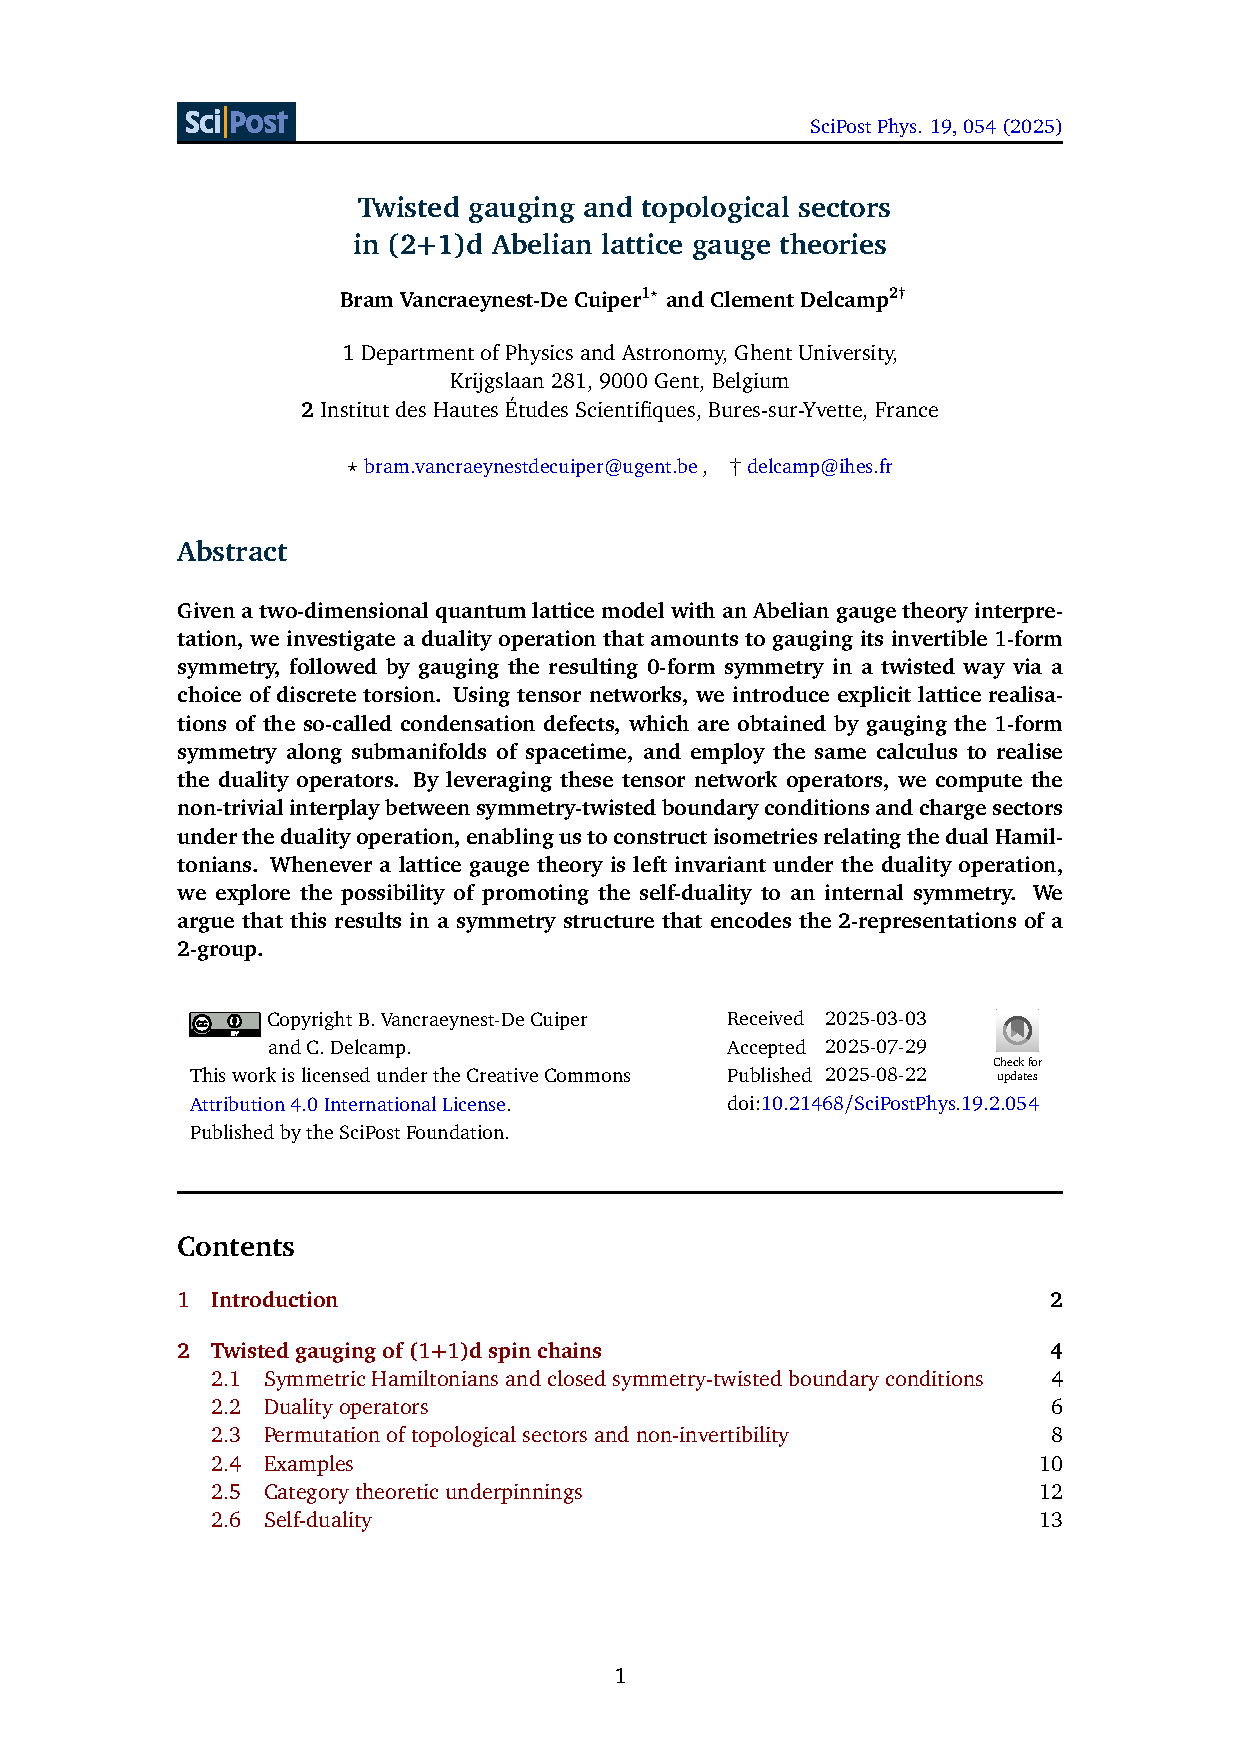
\includepdf[pages=-,
trim=25mm 20.54mm 25mm 17mm, clip=true,
noautoscale=true, height=\textheight,
offset=-0.65mm 4mm,
pagecommand={\thispagestyle{publication}}]{papers/twisted_gauging}

\chapter{Conclusions and outlook}
The central theme of this thesis has been the concrete tensor network realisation and study of various (generalised) symmetry structures. In conclusion, tensor networks provide a natural and effective framework in which these generalised symmetries can be explicitly represented on the lattice and manipulated. Not only do tensor networks provide a graphical calculus for dealing with these symmetries analytically, they also make it possible to put models with such symmetries on a computer and obtain their low-lying spectrum using variational methods. We reviewed this formalism from the ground up and illustrated it through several applications and research results.

Concretely, we saw that by phrasing topological order in the language of tensor networks, one can reveal hidden symmetry structures acting on the virtual degrees of freedom encoding the entanglement of the ground states. These symmetry structures are naturally described by fusion categories and realised as matrix product operators. Their relevance for the description of topological phases of matter can hardly be overstated. We demonstrated that they can be used naturally to construct distinct ground states as well as excited states, and argued that these symmetries persist beyond renormalisation fixed points.

In essence, these fusion categories describe simple symmetry operators, their fusion rules, and their anomalies. They therefore naturally generalise finite group and representation theory. Constructing all distinct representations of these categorical symmetries however requires bimodule categories. Although these may appear abstract at first sight, we have shown their importance in the construction of gapped boundaries of string-net models, and we have used them in the construction of a concrete quantum circuit that maps between Morita equivalent string-net models belonging to the same topological phase.

We then argued that these categorical symmetries also arise as internal symmetries of general Hamiltonians or classical models in one lower dimension. This holographic perspective allowed us to construct symmetric Hamiltonians, understand duality transformations as changes of module category, and relate the resulting dual models via bimodule tubes.

Finally, we showed that the same holographic tensor network perspective extends naturally to one higher dimension. We have shown that the symmetries of the (2+1)-dimensional models considered here are encoded in fusion 2-categories. This provides a higher-dimensional analogue of the categorical symmetry and duality framework developed earlier in the thesis.

\bigskip\noindent Within this framework, a number of open questions persist. Some of which, that spark my own interest, are the following.

One low-hanging fruit is to incorporate open boundary conditions into the symmetry and duality framework. In essence, this amounts to classifying the different ways in which symmetry operators can terminate at a physical boundary, and at the same time constructing the corresponding symmetric boundary Hamiltonian terms. This is particularly relevant for critical lattice models, where the infinite correlation length makes the bulk physics highly sensitive to the choice of boundary conditions~\cite{Fuchs2002,Thorngren2019,Choi2023,Lootens2022}.

From a technical point of view, module categories are expected to classify such boundary conditions in one dimension, and module 2-categories in two dimensions. However, it remains to understand how this classification interacts with the bulk degrees of freedom, and how to explicitly construct the corresponding boundary tensors for both the MPO and PEPO symmetries and the Hamiltonians.

Once such boundary conditions are incorporated, the next question is how to classify and explicitly construct the corresponding topological sectors, and how these sectors are mapped under duality transformations. This is particularly relevant for the numerical study of these open lattice models. Although the categorical structures expected to classify these sectors are formally known, turning this classification into an explicit tensor network construction remains an important open problem~\cite{Bullivant2020,Bullivant2021,Lootens2022}.

Also, it remains largely unexplored how to construct integrable lattice models with categorical symmetries within the tensor network formalism. In the main text, we only briefly touched upon the more natural setting for this question, namely two-dimensional classical lattice models. Such models can be constructed using the strange correlator construction which provides a systematic way of generating MPO symmetric transfer matrices depending on only a small number of parameters. The natural question is then which models within this low-dimensional family are (Yang-Baxter) integrable, and hence exactly solvable.

One promising approach is that of discrete holomorphicity, which imposes consistency equations on the Boltzmann weights guaranteeing the existence of a conserved current~\cite{Fendley2020}. It was shown how this naturally leads to known families of solutions to the Yang-Baxter equation. An interesting extension of the existing framework would be to allow currents described not by the input category itself, but by its Drinfeld center, thereby also covering input categories that are not braided. This is reminiscent of recent progress on the construction of critical lattice models with exotic symmetries~\cite{Huang2021,Vanhove2021b}.

By employing the tensor network formalism, it becomes possible to study these models numerically and potentially reconstruct the full conformal field theory spectrum from the obtained lattice models.



\bibliographystyle{BramBibStyle}
\bibliography{refs}
\end{document}